\documentclass[12pt,a4paper]{report}

% --- Multi-Engine Font and Language Support (English) ---
\usepackage{iftex}
\ifPDFTeX
  \usepackage[utf8]{inputenc}
  \usepackage[T1]{fontenc}
  \usepackage[english]{babel}
  \usepackage{newtxtext,newtxmath}
\else
  \usepackage{fontspec}
  \usepackage[english]{babel}
  % Use Times New Roman if available on system; otherwise use TeX Gyre Termes (TeX Live standard Times clone)
  \IfFontExistsTF{Times New Roman}{%
    \setmainfont{Times New Roman}%
  }{%
    \setmainfont{TeX Gyre Termes}%
  }
\fi

% --- Page Geometry (HCMUT Standard: Left 30mm, Right 20mm, Top 20mm, Bottom 20mm) ---
\usepackage[a4paper, left=30mm, right=20mm, top=20mm, bottom=20mm]{geometry}

% --- Line Spacing and Paragraph Formatting ---
\usepackage{setspace}
\onehalfspacing
\setlength{\parindent}{1.5em}
\setlength{\parskip}{0.35em}

% --- Header and Footer Formatting ---
\usepackage{fancyhdr}
\pagestyle{fancy}
\fancyhf{}
\cfoot{\thepage}
\renewcommand{\headrulewidth}{0pt}
\renewcommand{\footrulewidth}{0pt}

% Force plain pagestyle on chapter pages to match
\fancypagestyle{plain}{
  \fancyhf{}
  \cfoot{\thepage}
  \renewcommand{\headrulewidth}{0pt}
  \renewcommand{\footrulewidth}{0pt}
}

% --- Graphics and TikZ (Used for Cover Borders) ---
\usepackage{graphicx}
\usepackage{tikz}
\usetikzlibrary{calc}

% --- Advanced Tables ---
\usepackage{booktabs}
\usepackage{xltabular}
\usepackage{tabularx}
\usepackage{longtable}
\usepackage{array}
\usepackage{multirow}
\usepackage{makecell}

% --- Math and Symbols ---
\usepackage{amsmath,amssymb}

% --- Code Listings ---
\usepackage{listings}
\usepackage{xcolor}

\definecolor{codegreen}{rgb}{0,0.55,0}
\definecolor{codegray}{rgb}{0.45,0.45,0.45}
\definecolor{codepurple}{rgb}{0.55,0,0.75}
\definecolor{codeback}{rgb}{0.97,0.97,0.98}
\definecolor{codeframe}{rgb}{0.85,0.85,0.88}

\lstdefinestyle{bearbuddystyle}{
    backgroundcolor=\color{codeback},   
    commentstyle=\color{codegreen}\itshape,
    keywordstyle=\color{blue!80!black}\bfseries,
    numberstyle=\tiny\color{codegray},
    stringstyle=\color{codepurple},
    basicstyle=\ttfamily\footnotesize,
    breakatwhitespace=false,         
    breaklines=true,                 
    captionpos=b,                    
    keepspaces=true,                 
    numbers=none,                    
    showspaces=false,                
    showstringspaces=false,
    showtabs=false,                  
    tabsize=2,
    frame=single,
    rulecolor=\color{codeframe}
}
\lstset{style=bearbuddystyle}

% --- Captions and Hyperlinks ---
\usepackage{caption}
\captionsetup{font=small, labelfont=bf, labelsep=colon}

\usepackage{hyperref}
\hypersetup{
    colorlinks=true,
    linkcolor=blue!75!black,
    citecolor=blue!75!black,
    urlcolor=blue!75!black,
    bookmarksnumbered=true,
    bookmarksopen=true,
    pdfauthor={Bear Buddy Development Team},
    pdftitle={Bear Buddy - Software Requirement Specification and System Architecture}
}

% --- Section Numbering & TOC Depth ---
\setcounter{tocdepth}{3}
\setcounter{secnumdepth}{3}

\begin{document}

% ==================== FRONT MATTER ====================
\pagenumbering{roman}

% Cover page
\begin{titlepage}
\begin{tikzpicture}[remember picture, overlay]
    % Outer border: left 30mm, right 20mm, top 20mm, bottom 20mm
    \draw[line width=1.5pt] 
        ([xshift=30mm, yshift=-20mm]current page.north west) 
        rectangle 
        ([xshift=-20mm, yshift=20mm]current page.south east);
    % Inner border: 1mm inside outer border
    \draw[line width=0.6pt] 
        ([xshift=31mm, yshift=-21mm]current page.north west) 
        rectangle 
        ([xshift=-21mm, yshift=21mm]current page.south east);
\end{tikzpicture}

\centering
\vspace*{-0.8cm}

{\fontsize{15pt}{18pt}\selectfont \textbf{VIETNAM NATIONAL UNIVERSITY HO CHI MINH CITY}\par}
\vspace{0.25cm}
{\fontsize{15pt}{18pt}\selectfont \textbf{HO CHI MINH CITY UNIVERSITY OF TECHNOLOGY}\par}
\vspace{0.25cm}
{\fontsize{15pt}{18pt}\selectfont \textbf{FACULTY OF COMPUTER SCIENCE AND ENGINEERING}\par}

\vspace{1.2cm}

\begin{figure}[h!]
    \centering
    
\includegraphics[width=4.2cm]{figures/hcmut_logo.png}
\end{figure}

\vspace{1.0cm}

{\fontsize{15pt}{18pt}\selectfont \textbf{SOFTWARE REQUIREMENT SPECIFICATION}\par}
\vspace{0.25cm}
{\fontsize{15pt}{18pt}\selectfont \textbf{SEMESTER 252 ACADEMIC YEAR 2025--2026}\par}

\vspace{0.8cm}

\noindent\rule{0.88\textwidth}{1.2pt}
\vspace{0.25cm}

{\fontsize{20pt}{24pt}\selectfont \textbf{BEAR BUDDY}\par}
\vspace{0.2cm}
{\fontsize{20pt}{24pt}\selectfont \textbf{APPLICATION}\par}

\vspace{0.25cm}
\noindent\rule{0.88\textwidth}{1.2pt}

\vspace{0.6cm}

{\fontsize{14pt}{17pt}\selectfont \textbf{COURSE: MOBILE APPLICATION DEVELOPMENT (CO3041)}\par}

\vspace{0.8cm}

\begin{flushleft}
\hspace{1.8cm}
\begin{tabular}{ll}
    \textbf{ADVISOR:} & PhD. Phan Trần Minh Khuê \\[0.25cm]
    \textbf{GROUP:}   & CC01 -- 03 \\[0.25cm]
    \textbf{STUDENT 1:} & Nguyễn Tiến Khang -- 2252304 \\[0.25cm]
    \textbf{STUDENT 2:} & Trần Nguyễn Anh Khoa -- 2252364 \\[0.25cm]
    \textbf{STUDENT 3:} & Ôn Đức Phát -- 2352897 \\[0.25cm]
    \textbf{STUDENT 4:} & Phan Quang Minh -- 2252486 \\
\end{tabular}
\end{flushleft}

\vfill

{\fontsize{14pt}{17pt}\selectfont \textbf{HO CHI MINH CITY, MAY 2026}\par}
\vspace{0.5cm}

\end{titlepage}



% Member contributions table
\chapter*{Member Contributions}
\addcontentsline{toc}{chapter}{Member Contributions}
\thispagestyle{plain}

\vspace{0.8cm}

\noindent
\begin{table}[htbp]
\centering
\renewcommand{\arraystretch}{1.5}
\begin{tabularx}{\textwidth}{|p{3.8cm}|c|X|c|}
\hline
\textbf{Name} & \textbf{Student ID} & \textbf{Main Contributions} & \textbf{Completion} \\
\hline
Nguyễn Tiến Khang & 2252304 & System architecture, frontend and backend implementation, AI assistant integration, database design, UI-UX design, testing, and documentation. & 100\% \\
\hline
Ôn Đức Phát & 2352897 & Frontend development, API integration, audio and speech interaction features, testing, and documentation. & 100\% \\
\hline
Trần Nguyễn Anh Khoa & 2252364 & Backend development, database integration, authentication features, testing, and deployment support. & 100\% \\
\hline
Phan Quang Minh & 2252486 & Market research, UI-UX prototyping, user evaluation, report formatting, and presentation preparation. & 100\% \\
\hline
\end{tabularx}
\end{table}

\vfill
\clearpage


% Table of Contents
\tableofcontents
\clearpage

% List of Figures
\listoffigures
\clearpage

% List of Tables
\listoftables
\clearpage

% ==================== MAIN MATTER ====================
\pagenumbering{arabic}
\setcounter{page}{1}

% Chapter 1: Introduction
\chapter{Introduction}

\section{Application Description}

Bear Buddy is a mobile application designed to support autistic children in becoming familiar with and navigating everyday social situations through short stories, illustrations, spoken narration, and interactive learning activities. The application is conceptualized as a situational learning tool in which children can explore contexts, predict narrative developments, choose responses, and receive clear explanations before encountering similar real-world scenarios.

The content of Bear Buddy is structured following the principles of the Social Story methodology and enriched with interactive engagement. Initial situational scenarios cover waiting for one's turn, greeting new peers, asking to join group play, and requesting assistance. The topic library can be expanded to encompass specific everyday contexts such as visiting a physician, getting a haircut, changing classrooms, or coping when a request is declined.

During a typical learning session, a parent or support teacher selects an appropriate social story, introduces the activity, and provides scaffolding as needed. The child directly views, listens to, and interacts with the story frames. Each critical decision point is connected to character reactions and pre-authored explanations, clarifying the explicit relationship between an action, its social reaction, and the underlying rationale. The interaction history is recorded to enable caregivers to review learning engagement, discuss experiences with the child, and plan subsequent developmental activities.

Bear Buddy defines two primary user groups. The primary user is the child who directly experiences the interactive story. The secondary user is the parent or support teacher who configures assistive settings, selects content, and reviews session outcomes. Throughout this report, the term \textit{caregiver} refers collectively to adult companions; specific role permissions for parents and teachers are formally specified in Chapter~3.

Artificial Intelligence (AI) is utilized in two bounded scopes: assisting caregivers in discovering stories matched to developmental goals or past interaction patterns, and supporting bounded voice interaction in Scenario~E. Because Scenario~E represents an experimental speech interaction paradigm, this report establishes a strict touch fallback so that the core learning loop remains fully accessible through touch manipulation and pre-authored story assets whenever speech recognition is disabled.

\section{Problem Statement}

Many autistic children experience difficulties in interpreting implicit social cues that are not communicated directly, such as facial expressions, vocal prosody, conversational turn-taking, or the underlying reasons why others react to specific behaviors. In common social scenarios such as waiting for a turn, greeting a peer, asking to join a game, or asking for help, recognizing individual vocabulary words is often insufficient to comprehend the complete social context. Documentation from the National Institutes of Health (NIH) emphasizes the wide diversity in communication profiles and the cognitive barriers autistic individuals may face when deciphering subtle communicative signals.

The research hypothesis of this project posits that in many home and classroom environments, behavioral guidance currently relies on reactive explanations delivered at the moment a social difficulty arises. Such ad-hoc explanations tend to be fragmented, vary significantly between different adult caregivers, and lack structured permanence for repeated review. Furthermore, adults cannot consistently anticipate and explain every subtle cue in real time. This hypothesis motivates our formal requirements elicitation and system design.

From this problem hypothesis, three primary gaps have been identified:
\begin{enumerate}
    \item Children require a structured, predictable, and repeatable mechanism to explore social situations in a low-anxiety environment.
    \item Adult caregivers require pre-authored, standardized content to provide consistent scaffolding across home and school settings.
    \item Caregivers need clear visibility into how children make choices and understand rationales, rather than merely tracking completion counts.
\end{enumerate}

The proposed solution transforms prevalent social scenarios into interactive, pre-structured digital social stories. Children encounter each component of a situational context step-by-step, observe potential behavioral responses and their social consequences, and engage in penalty-free retries with appropriate scaffolding. Character reactions represent natural conversational dynamics rather than punitive scoring, helping children construct cause-and-effect mental models without fear of failure.

\section{Project Goals and Objectives}

The primary goal of the Bear Buddy project is to design, specify, and architect an accessible mobile application that assists autistic children in exploring everyday social scenarios through interactive social stories, accompanied by adult configuration and review tools.

To achieve this goal, the project establishes four concrete objectives:
\begin{enumerate}
    \item \textbf{Develop a Structured Social Story Engine}: Deliver an interactive story player based on Carol Gray's Social Story criteria, incorporating clear visual representations, single-stream narration, and predictable scene transitions.
    \item \textbf{Implement a Predictable, Non-Punitive Learning Loop}: Formulate an interaction loop (\textit{Understand $\rightarrow$ Predict $\rightarrow$ Choose $\rightarrow$ Observe $\rightarrow$ Understand Why $\rightarrow$ Repeat}) that reinforces cause-and-effect understanding without penalizing incorrect choices.
    \item \textbf{Provide Role-Separated Caregiver Scaffolding}: Establish a dedicated Caregiver Mode protected by authentication (\texttt{Caregiver Gate}) to manage child profiles, configure accessibility settings, generate teacher access links, and review version-pinned session logs.
    \item \textbf{Design for Offline-First Accessibility and Privacy}: Architect an offline-first mobile system utilizing local SQLite storage, strict on-device data minimization, transparent microphone consent, and comprehensive accessibility adaptations (WCAG~2.2 AA touch targets, high contrast, and font scaling).
\end{enumerate}

\section{Target Audience and Scope}

\subsection{Target Audience and Developmental Profiles}

Bear Buddy primarily targets children aged 4 to 10 with developmental differences on the autism spectrum, characterized by:
\begin{itemize}
    \item Verbal or minimally verbal communication capabilities, capable of comprehending short sentences and concrete visual icons.
    \item Emerging ability to perform direct single-touch selection on a touchscreen interface.
    \item A need for high predictability, explicit cause-and-effect demonstration, and minimal sensory distraction.
\end{itemize}

Secondary target users comprise parents, primary family caregivers, and special education teachers who accompany and support the child's learning process.

\subsection{Planned Functional Scope}

The planned functional scope of the Bear Buddy application is organized into core functional modules as summarized in Table~\ref{tab:c1_functional_scope}.

\begin{xltabular}{\textwidth}{|p{4.2cm}|X|}
\hline
\textbf{Functional Group} & \textbf{Scope and Technical Deliverables} \\ \hline
\endhead
\textbf{Story Library \& Categorization} & Standardized situational categories (Peer Interaction, Routine Changes, Emotional Regulation, Classroom Tasks) with versioned metadata. \\ \hline
\textbf{Interactive Story Player} & Single-stream audio narration, synchronized visual frames, explicit social cue callouts, and tap-based decision activities. \\ \hline
\textbf{Feedback \& Rationale} & Character reaction displays and explicit ``Why'' explanations (\texttt{S11}, \texttt{S12}); non-punitive retry loops. \\ \hline
\textbf{Voice Interaction (Scenario~E)} & Bounded on-device speech recognition for simple affirmative utterances with mandatory touch fallback. \\ \hline
\textbf{Session History \& Review} & Version-pinned logging of choices, attempts, and durations for caregiver inspection (\texttt{S15}, \texttt{S16}). \\ \hline
\textbf{AI Recommendation Engine} & Explainable hybrid grounded story recommendations for caregivers based on child profile and learning history. \\ \hline
\textbf{Profiles \& Role Access} & Caregiver authentication gate, multi-child profile management, and teacher access link delegation. \\ \hline
\textbf{Local Storage \& Persistence} & Offline-first SQLite database architecture ensuring core learning continuity without cloud dependency. \\ \hline
\textbf{Onboarding \& Orientation} & Product introduction, caregiver verification setup, and child orientation sequence (\texttt{S08}). \\ \hline
\textbf{Accessibility Adaptations} & Dynamic Type font scaling, minimum 48dp touch targets, high-contrast palette, and sound toggles. \\ \hline
\textbf{Privacy \& Data Security} & Granular consent audit logging, local data encryption, and transparent microphone permissions. \\ \hline
\textbf{Help, Support \& Feedback} & In-app FAQ, caregiver guidance documentation, and structured issue reporting. \\ \hline
\end{xltabular}
\label{tab:c1_functional_scope}

\subsection{Operational Scope and Constraints}

Bear Buddy is designed for use in quiet home or structured educational settings under adult guidance. The digital companion serves as a preparatory and consolidation aid; it does not replace direct adult supervision or clinical therapy.

The initial release targets the iOS platform (iOS 17+) using native SwiftUI, with an architecture extensible to cross-platform deployments. Initial content is provided in Vietnamese and English, with localization infrastructure established in the database schema to accommodate future languages.

\section{User Flow Overview}

The primary user flow follows an adult-guided companion model:
\begin{center}
\textbf{Caregiver Selects Story} $\longrightarrow$ \textbf{Child Explores Context} $\longrightarrow$ \textbf{Decision Activity} $\longrightarrow$ \textbf{Observe Reaction \& Why} $\longrightarrow$ \textbf{Consolidation / Retry} $\longrightarrow$ \textbf{Caregiver Review}
\end{center}

This macro-flow operationalizes into six discrete interaction steps:
\begin{enumerate}
    \item \textbf{Setup and Verification}: The adult caregiver completes onboarding, verifies access via the Caregiver Gate, selects the active child profile, and adjusts accessibility preferences.
    \item \textbf{Story Selection}: The caregiver browses categorized stories or consults explainable AI suggestions, previews learning objectives, and initiates the session.
    \item \textbf{Context Presentation}: The child views the scene illustration and listens to clear, single-stream narration describing the setting, participants, and explicit social cues.
    \item \textbf{Decision Activity}: The child predicts an appropriate behavioral response by tapping a choice card or, in Scenario~E, speaking a short phrase.
    \item \textbf{Outcome Observation and Explanation}: The application displays the character's natural reaction and provides a concrete explanation of why that outcome occurred, offering penalty-free replaying or retrying.
    \item \textbf{Review and Planning}: The caregiver inspects the version-pinned session record, discusses takeaways with the child, and schedules subsequent learning reminders.
\end{enumerate}

The core learning loop is defined as \textbf{Understand $\rightarrow$ Predict $\rightarrow$ Choose $\rightarrow$ Observe $\rightarrow$ Understand Why $\rightarrow$ Repeat}. Retrying is entirely optional and free from negative scores or interaction penalties.

\section{User-Centered Design Orientation}

All interaction and visual decisions in Bear Buddy are governed by a four-layer UX Reasoning Framework:
\begin{center}
\textbf{User Characteristics} $\longrightarrow$ \textbf{UX Concerns} $\longrightarrow$ \textbf{UX Principles} $\longrightarrow$ \textbf{Design Decisions}
\end{center}

The developmental profiles and personas detailed in Chapter~2 provide the fundamental inputs. Chapter~5 translates these requirements into interface tokens, component behaviors, and screen layouts. In accordance with W3C Web Accessibility Initiative (WAI) guidelines on user-centered accessibility, prototype evaluations and user feedback directly inform iterative refinements to both specifications and software architecture.


% Chapter 2: Background and Related Work
\chapter{Background and Related Work}

\section{Target User Group Characteristics}

\subsection{Children and Developmental Diversity}

Child development encompasses interconnected domains including receptive and expressive language, social cognition, sensory processing, fine motor coordination, and executive functioning. In early and middle childhood (ages 4--10), children acquire communicative competencies primarily through observation, concrete modeling, and guided social interactions. However, children exhibit wide variations in developmental pace, cognitive processing styles, and emotional regulation thresholds. Designing interactive software for this demographic necessitates structured predictability, intuitive affordances, and cognitive load minimization.

\subsection{Autism Spectrum and Diversity of Competency Profiles}

Autism Spectrum Disorder (ASD) is characterized by persistent differences in social communication and interaction, alongside restricted or repetitive patterns of behavior, interests, or activities~\cite{cdc_diagnosis, nih_asd}. Individuals on the autism spectrum demonstrate heterogeneous developmental profiles; capabilities vary significantly across cognitive, linguistic, sensory, and motor dimensions. Table~\ref{tab:c2_asd_dimensions} delineates key developmental dimensions and their corresponding implications for digital system design.

\begin{xltabular}{\textwidth}{|p{4.0cm}|X|}
\hline
\textbf{Developmental Dimension} & \textbf{Observed Difficulties and System Design Implications} \\ \hline
\endhead
\textbf{Social Understanding} & Autistic children frequently require explicit scaffolding to interpret facial expressions, vocal prosody, subtle intentions, or conversational turn-taking rules. The system must render implicit social cues concrete and visible. \\ \hline
\textbf{Communication} & Expressive abilities range from non-verbal and minimally verbal to fluent speech. Metaphorical language, sarcasm, and ambiguous instructions elevate cognitive anxiety. Interfaces must rely on concise, literal sentences and visual symbols. \\ \hline
\textbf{Predictability \& Routine} & Sudden changes in activity or unclear sequences can trigger distress. Clear procedural progression, persistent forward/backward controls, and activity previews foster psychological safety. \\ \hline
\textbf{Sensory Processing} & Atypical sensory reactivity is prevalent~\cite{cdc_symptoms}. Overlapping auditory stimuli, rapid animations, or flashing visual elements risk sensory overload. Auditory and visual outputs must remain single-stream and configurable. \\ \hline
\textbf{Repetitive Behaviors \& Focused Interests} & Structured repetition supports consolidation and emotional stabilization. The application must permit penalty-free replaying and retrying of narrative steps without timer pressure. \\ \hline
\textbf{Executive Function \& Emotion Regulation} & Difficulties with working memory and cognitive flexibility make complex multi-step choices frustrating. Options must be limited to 2--3 discrete, distinct choices per interaction point. \\ \hline
\end{xltabular}
\label{tab:c2_asd_dimensions}

\subsection{Prioritized Developmental Competency Profile}

To ensure high internal validity and focused UX execution, Bear Buddy prioritizes a specific developmental competency profile:
\begin{itemize}
    \item \textbf{Age}: 4 to 10 years old.
    \item \textbf{Language Level}: Verbal or minimally verbal learners who comprehend simple spoken phrases and recognize common pictorial representations, but do not yet rely on independent reading for task completion.
    \item \textbf{Motor Competence}: Capable of gross single-finger taps on large touch targets, while experiencing instability with fine multi-finger gestures, precision dragging, or prolonged holding.
    \item \textbf{Cognitive Need}: Requires concrete cause-and-effect demonstration connecting personal actions to peer/adult reactions and explicit reasons.
\end{itemize}

\section{Foundations of the Social Story Methodology}

\subsection{Origins and Purpose}

The Social Story methodology was developed by Carol Gray in the early 1990s as a structured psychoeducational intervention to share accurate social information with autistic individuals~\cite{gray_overview, gray_what_is}. Rather than functioning as a compliance tool or behavioral modification script, a authentic Social Story aims to describe social situations objectively, highlighting relevant social cues, perspectives, and potential responses in a reassuring, respectful tone. Clinical trials and systematic reviews, including the ASSIST2 randomized controlled trial~\cite{wright_assist2_2024}, indicate that structured social stories support social understanding and emotional well-being when authored with fidelity to standardized criteria.

\subsection{Structure and Linguistic Criteria}

According to the Social Stories 10.4 criteria~\cite{gray_criteria_2023}, an authentic social story must maintain a supportive, patient tone and balance sentence types according to the \textit{Social Story Formula}:
\begin{equation}
\frac{\text{Descriptive} + \text{Perspective} + \text{Affirmative Sentences}}{\text{Directive / Coaching Sentences}} \ge 2
\end{equation}
This formula ensures that descriptive and reassuring statements significantly outnumber directive instructions. Table~\ref{tab:c2_sentence_types} outlines how these sentence functions are operationalized in Bear Buddy.

\begin{xltabular}{\textwidth}{|p{4.0cm}|X|}
\hline
\textbf{Sentence Function} & \textbf{Operationalization in Bear Buddy Stories} \\ \hline
\endhead
\textbf{Descriptive Sentences} & Provide objective factual information regarding the setting, participants, and visible actions (e.g., ``The children are playing with blocks on the carpet.''). \\ \hline
\textbf{Perspective Sentences} & Describe the internal feelings, thoughts, or reactions of characters in an empathetic manner (e.g., ``My classmate feels happy when we take turns.''). \\ \hline
\textbf{Directive / Coaching} & Offer gentle, flexible behavioral suggestions rather than rigid demands (e.g., ``I can try tapping my friend's shoulder to ask for a turn.''). \\ \hline
\textbf{Affirmative Sentences} & Reassure the learner and validate common values or shared experiences (e.g., ``It is okay to feel disappointed when waiting is hard.''). \\ \hline
\end{xltabular}
\label{tab:c2_sentence_types}

\subsection{Content Preparation and Personalization Workflow}

Applying social stories effectively requires personalized preparation:
\begin{enumerate}
    \item \textbf{Context Elicitation}: Identifying the specific trigger or unfamiliar situation causing anxiety (e.g., transitioning between activities).
    \item \textbf{Information Gathering}: Determining the child's perspective, sensory sensitivities, and preferred visual cues.
    \item \textbf{Text Drafting}: Composing short, affirmative sentences respecting the 10.4 ratio criteria.
    \item \textbf{Multimodal Pairing}: Associating each sentence with a concrete visual frame and clear audio narration.
    \item \textbf{Guided Review and Rehearsal}: Introducing the story in a calm environment prior to facing the real-world event.
\end{enumerate}

\subsection{Illustrative Scenario: Visiting the Doctor}

Consider an unfamiliar clinical visit. A conventional approach might offer verbal reminders during the examination, often overwhelming the child. A structured Bear Buddy story breaks the experience into predictable segments:
\begin{enumerate}
    \item \textit{Waiting Room}: ``The clinic has chairs and books. People wait quietly until their name is called.''
    \item \textit{Instruments}: ``The doctor uses a stethoscope. It feels cool on my chest for a few seconds.''
    \item \textit{Cooperative Action}: ``I can sit still on the examination table while the doctor listens.''
    \item \textit{Closure}: ``When the checkup is finished, I can return home with my parent.''
\end{enumerate}

\subsection{Application in Bear Buddy and Evidence Boundaries}

Bear Buddy translates the traditional paper booklet format into an interactive digital application. However, academic integrity requires distinguishing between verified clinical evidence and interactive design hypotheses:
\begin{itemize}
    \item \textbf{Established Evidence}: The efficacy of visual narratives and social stories in reducing anxiety and clarifying expectations is well documented in special education literature~\cite{gray_criteria_2023, wright_assist2_2024}.
    \item \textbf{Interactive Hypotheses}: Incorporating digital decision points, branching consequence animations, and voice practice represents an interactive software hypothesis designed to enhance engagement, which requires empirical validation through user testing.
\end{itemize}

\section{Multimodal Learning via Visuals, Narration, and Interaction}

\subsection{Concrete Visual Representations}

Visual stimuli provide cognitive anchoring for children who experience difficulties with auditory language processing. In Bear Buddy:
\begin{itemize}
    \item Characters are illustrated with clear, unambiguous facial expressions and posture.
    \item Irrelevant background clutter and motion visual noise are eliminated.
    \item Interactive targets are highlighted with distinct outlines and high-contrast bounding boxes.
\end{itemize}

\subsection{Short Sentences and Audio Narration}

To accommodate varying reading abilities, all on-screen text is paired with professional, synchronized single-stream audio narration. The narration utilizes:
\begin{itemize}
    \item Natural, calm pacing (110--125 words per minute).
    \item Clear articulation without background music or sound effects that could mask spoken dialogue.
    \item Complete user control to pause, resume, or replay audio segments at will.
\end{itemize}

\subsection{Interactive Engagement and Cause-and-Effect Relationships}

Unlike passive video watching or static reading, interactive selection requires active cognitive participation. By choosing a response (e.g., tapping ``Ask politely'' vs.\ ``Grab the toy''), the child directly observes the resulting social reaction and the underlying ``Why'' explanation. This immediate feedback loop operationalizes Piagetian schema modification in a risk-free simulation.

\subsection{Channel Coordination and Cognitive Load Limits}

Simultaneous multimedia channels can induce split-attention effects. In Bear Buddy:
\begin{itemize}
    \item Audio and visual streams are strictly synchronized to describe the same conceptual focal point.
    \item Decision options appear only after the scene narration completes, preventing visual distraction during context setup.
    \item Sound effects are restricted to gentle auditory chimes confirming selection, avoiding loud or startling tones.
\end{itemize}

\section{Personas and Developmental Capability Profiles}

\subsection{Persona PERS01: Minh (Primary Child Learner)}

\begin{xltabular}{\textwidth}{|p{4.0cm}|p{4.5cm}|X|}
\hline
\textbf{Competency Dimension} & \textbf{Observed Persona Characteristic} & \textbf{System Design Scaffolding} \\ \hline
\endhead
\textbf{Language Comprehension} & Understands short, concrete phrases in familiar settings; struggles with compound sentences. & Single-clause sentences ($<12$ words); single-stream narration (\texttt{DD7}, \texttt{DD8}). \\ \hline
\textbf{Expressive Communication} & Primarily indicates preferences by pointing/tapping; emerging short verbal responses. & Touch card selection with large tap boundaries; optional voice practice (\texttt{DD26}, \texttt{DD27}). \\ \hline
\textbf{Visual Recognition} & Readily recognizes familiar objects and everyday actions; abstract symbols cause confusion. & High-clarity concrete illustrations without decorative visual clutter (\texttt{DD11}). \\ \hline
\textbf{Reading Competence} & Emergent reader; cannot rely on textual cues alone for activity progression. & Mandatory audio narration accompanied by text highlighting (\texttt{DD10}). \\ \hline
\textbf{Attention \& Transition} & Distracted by competing animations or sudden auditory shifts. & Predictable scene templates; no background audio tracks (\texttt{DD20}, \texttt{DD22}). \\ \hline
\textbf{Cause-and-Effect} & Successfully links actions to outcomes when explicitly demonstrated step-by-step. & Explicit three-part feedback sequence: Action $\rightarrow$ Reaction $\rightarrow$ Why explanation (\texttt{DD13}, \texttt{DD14}). \\ \hline
\textbf{Motor Coordination} & Capable of direct single taps; precision dragging or pinch gestures are erratic. & Minimum 56dp tap targets; no multi-touch, drag-and-drop, or timed tap demands (\texttt{DD28}, \texttt{DD30}). \\ \hline
\textbf{Sensory Sensitivity} & Startled by sudden loud noises or flashing screen transitions. & Soft color palette; gradual crossfades; no jarring alarm sounds (\texttt{DD21}, \texttt{DD23}). \\ \hline
\textbf{Regulation \& Agency} & May disengage or seek adult assistance when overwhelmed. & Prominent ``Take a Break'' and ``Need Help'' buttons available on all child screens (\texttt{DD37}). \\ \hline
\textbf{Adult Scaffolding} & Benefits from adult co-viewing during initial exposure to unfamiliar stories. & Role-separated Caregiver Mode allowing parents to preview content and review attempts (\texttt{DD31}). \\ \hline
\end{xltabular}
\label{tab:c2_persona_minh}

\subsection{Persona PERS02: Ms. An (Primary Parent Companion)}

Ms.~An is the mother of 6-year-old Minh. She works full-time and coordinates home developmental exercises in the evening. Her core goals include:
\begin{itemize}
    \item Finding reliable, evidence-informed digital tools that reinforce positive social communication.
    \item Preparing Minh for upcoming school events or routine disruptions without generating anxiety.
    \item Gaining visibility into Minh's progress and understanding which social concepts require reinforcement.
    \item Ensuring her child's voice and behavioral data remain strictly private and securely stored on the local device.
\end{itemize}

\subsection{Persona PERS03: Ms. Mai (Special Education Support Teacher)}

Ms.~Mai is an inclusion support educator working with autistic elementary students. Her primary operational requirements are:
\begin{itemize}
    \item Selecting specific situational social stories aligned with weekly classroom behavioral objectives.
    \item Guiding structured 10-minute intervention sessions during school hours.
    \item Redeeming parent-delegated access links without accessing the family's private account or billing information.
    \item Reviewing interaction logs to discuss behavioral observations with parents during parent-teacher consultations.
\end{itemize}

\subsection{Testable Assumptions Derived from Personas}

The personas establish explicit assumptions to be validated through usability testing:
\begin{enumerate}
    \item A single-touch tap interface is sufficient for autistic children within the target motor competency profile to navigate story decisions without frustration.
    \item Explaining the causal ``Why'' behind peer reactions increases social concept retention compared to passive story presentation.
    \item Caregivers actively utilize session logs to facilitate follow-up verbal discussions with children.
\end{enumerate}

\section{Related Work Analysis}

\subsection{Comparative Methodology}

To position Bear Buddy within the assistive educational software landscape, we conducted a systematic evaluation of three prominent commercial and clinical applications: Pictello, Social Stories Creator and Library, and Choiceworks. The analysis evaluates authoring flexibility, interactive decision-making, feedback mechanisms, and caregiver review capabilities.

\subsection{Pictello (AssistiveWare)}

Pictello is a versatile visual storytelling application widely used in augmentative and alternative communication (AAC)~\cite{pictello}.
\begin{itemize}
    \item \textbf{Strengths}: Supports custom photo/video importation, synthetic text-to-speech, recorded voice narration, and story sharing via PDF or cloud accounts.
    \item \textbf{Limitations}: Stories are linear and passive. The application lacks interactive decision points, branching consequence exploration, and structured cause-and-effect review analytics.
\end{itemize}

\subsection{Social Stories Creator and Library (Touch Autism)}

Social Stories Creator and Library provides pre-made social stories alongside tools for custom book creation~\cite{social_stories_creator}.
\begin{itemize}
    \item \textbf{Strengths}: Library organized by pediatric social themes; intuitive page-turning interface; customizable text and images.
    \item \textbf{Limitations}: Reading is linear. Feedback is limited to page completion without interactive prediction activities or non-punitive decision reinforcement.
\end{itemize}

\subsection{Choiceworks (Bee Visual)}

Choiceworks focuses on daily visual schedules, waiting boards, and emotional choice-making~\cite{choiceworks}.
\begin{itemize}
    \item \textbf{Strengths}: Exceptional visual clarity for scheduling and emotional regulation; tangible drag-to-complete interactions; high predictability.
    \item \textbf{Limitations}: Structured as a task checklist rather than a situational social narrative. It does not provide narrative context or explicit causal explanations for interpersonal interactions.
\end{itemize}

\subsection{Synthesis and Strategic Positioning}

Table~\ref{tab:c2_related_work} synthesizes the comparative findings, highlighting Bear Buddy's unique integration of interactive social stories with explainable cause-and-effect learning.

\begin{xltabular}{\textwidth}{|p{3.2cm}|p{4.5cm}|X|}
\hline
\textbf{Application} & \textbf{Officially Documented Strengths} & \textbf{Gap Addressed by Bear Buddy} \\ \hline
\endhead
\textbf{Pictello} & Rich multimedia authoring, synthetic and natural speech playback, visual story sharing. & Implements interactive branching choices, explicit consequence displays, and non-punitive learning loops. \\ \hline
\textbf{Social Stories Creator} & Thematic story library, simple page-by-page presentation for pediatric users. & Integrates structured cause-and-effect reasoning (\textit{Action $\rightarrow$ Reaction $\rightarrow$ Why}) and caregiver review analytics. \\ \hline
\textbf{Choiceworks} & Highly effective visual schedules, waiting timers, and emotional regulation boards. & Embeds situational decision activities into full narrative contexts rather than isolated scheduling lists. \\ \hline
\end{xltabular}
\label{tab:c2_related_work}

\section{Requirements Elicitation and Validation Plan}

\subsection{Existing Evidence and Knowledge Gaps}

While current literature verifies the general benefits of social narratives and visual aids~\cite{gray_criteria_2023, wcag22}, critical empirical questions remain regarding digital interactive implementations:
\begin{itemize}
    \item How many choices can a child process simultaneously without experiencing cognitive overload?
    \item Does on-device speech practice in Scenario~E encourage verbal imitation, or does it elevate performance anxiety?
    \item What log granularity do caregivers require to conduct meaningful post-session discussions?
\end{itemize}

\subsection{Planned User Research Activities}

To address these knowledge gaps, the Bear Buddy development plan specifies three iterative research activities:
\begin{enumerate}
    \item \textbf{Expert Content Review}: Collaborating with special education practitioners and speech therapists to review story scripts against Carol Gray's 10.4 sentence criteria.
    \item \textbf{Co-Viewing Observational Sessions}: Observing parent-child dyads navigating interactive story modules to evaluate tap target ergonomics, pacing, and emotional responses.
    \item \textbf{Caregiver Review Interviews}: Evaluating whether parents and teachers find version-pinned session summaries actionable for individualized educational planning.
\end{enumerate}

\subsection{Mapping User Needs to Design Specifications}

Table~\ref{tab:c2_user_needs} maps the twelve elicited user needs (\texttt{UN01}--\texttt{UN12}) directly to the corresponding UI/UX design decisions (\texttt{DD1}--\texttt{DD40}) and architectural modules.

\begin{xltabular}{\textwidth}{|p{1.8cm}|p{4.5cm}|X|}
\hline
\textbf{User Need} & \textbf{Elicited User Requirement} & \textbf{Design Decision and Architectural Tracing} \\ \hline
\endhead
\textbf{UN01} & Comprehend situational context before being prompted to make decisions. & Explicit Scene Context screen establishing participants and environment (\texttt{DD13}, \texttt{DD14}, Screen \texttt{S09}). \\ \hline
\textbf{UN02} & Engage meaningfully with stories without requiring independent reading fluency. & Synchronized single-stream narration and concrete pictorial representations (\texttt{DD7}--\texttt{DD12}, Screen \texttt{S09}). \\ \hline
\textbf{UN03} & Maintain situational predictability and awareness of current activity progress. & Consistent step indicator, persistent navigation controls, and standardized screen templates (\texttt{DD2}--\texttt{DD6}). \\ \hline
\textbf{UN04} & Select choices without requiring fine motor precision or complex multi-touch gestures. & Large touch cards ($\ge 56\text{dp}$) with generous padding and single-tap selection (\texttt{DD26}--\texttt{DD30}, Screen \texttt{S10}). \\ \hline
\textbf{UN05} & Understand why social reactions occur and replay or retry without penalty. & Two-stage feedback displaying character reaction and explicit ``Why'' rationale (\texttt{DD15}--\texttt{DD19}, Screens \texttt{S11}, \texttt{S12}). \\ \hline
\textbf{UN06} & Regulate sensory stimulation and pacing according to individual sensitivity. & Dedicated accessibility controls for volume, contrast, font scaling, and animation speed (\texttt{DD20}--\texttt{DD25}). \\ \hline
\textbf{UN07} & Allow caregivers to search, filter, preview, and select developmentally matched stories. & Searchable situational library with objective previews in Caregiver Mode (\texttt{DD32}, \texttt{DD33}, Screens \texttt{S06}, \texttt{S07}). \\ \hline
\textbf{UN08} & Review accurate, version-pinned session records linked to specific child profiles. & Persistent session history recording exact story version, chosen options, and retry counts (\texttt{DD34}, Screen \texttt{S15}). \\ \hline
\textbf{UN09} & Understand the rationale behind AI recommendations and maintain full supervisory control. & Explainable grounded AI suggestions providing clear match reasoning with manual override (\texttt{DD35}, Screen \texttt{S05}). \\ \hline
\textbf{UN10} & Empower the child to pause the activity or request adult assistance at any moment. & Persistent, accessible ``Take a Break'' and ``Need Help'' controls (\texttt{DD37}, Screens \texttt{S09}--\texttt{S14}). \\ \hline
\textbf{UN11} & Ensure child data, voice inputs, and learning logs are protected with strict privacy. & Local-first data architecture, transparent microphone consent, and role separation (\texttt{DD31}, \texttt{DD36}, \texttt{DD38}). \\ \hline
\textbf{UN12} & Provide graceful error recovery and offline fallback when services are interrupted. & Automatic fallback to touch interaction and preserved local state on network loss (\texttt{DD39}, \texttt{DD40}). \\ \hline
\end{xltabular}
\label{tab:c2_user_needs}


% Chapter 3: Requirement Analysis
\chapter{Requirement Analysis}


This chapter presents the formal requirement analysis specification for the \textbf{Bear Buddy} application. It builds directly upon the problem statement in Chapter 1, the developmental capability profiles and user needs (\texttt{UN01}–\texttt{UN12}) in Chapter 2, and establishes a traceable foundation for story content design in Chapter 4, UI-UX design decisions (\texttt{DD1}–\texttt{DD40}, screens \texttt{S01}–\texttt{S24}) in Chapter 5, and system architecture in Chapter 6.


\section{Stakeholders and Roles}


The Bear Buddy system involves multiple stakeholder groups who either directly interact with the application or participate in content authoring, clinical/educational review, and technical operation. Role permissions are strictly separated to safeguard children's data privacy and prevent administrative complexity from leaking into the child's learning flow (\texttt{DD31}, \texttt{DD32}).


\subsection{Primary Stakeholders (Direct Users)}


\noindent\begin{xltabular}{\textwidth}{|p{2.0cm}|p{3.2cm}|X|p{2.8cm}|}
\hline
\textbf{Stakeholder} & \textbf{Persona Reference} & \textbf{System Role} & \textbf{Permissions and Access Boundaries} \\ \hline
\endhead
\textbf{Child Learner (Primary User)} & \texttt{PERS01} Minh & Direct participant who experiences social stories and practices interactive activities in \textbf{Child Mode}. & Accesses only the story session launched by a caregiver; views scenes, listens to narration, selects options, uses \texttt{Replay}, \texttt{Retry}, \texttt{Pause} (\textit{Take a Break}), or \texttt{Need Help}. Cannot access settings, profile management, or analytics. \\ \hline
\textbf{Parent (Primary Caregiver)} & \texttt{PERS02} Ms. An & Primary adult companion in \textbf{Caregiver Mode}, responsible for managing the child's profile and deciding learning content. & Full authority to create, edit, and delete child profiles under their guardianship; configures support and accessibility settings; selects stories, uses AI suggestions, reviews session logs, schedules reminders; grants or revokes teacher access links; manages data privacy and microphone permissions. \\ \hline
\textbf{Support Teacher (Authorized Caregiver)} & \texttt{PERS03} Ms. Mai & Adult companion in classroom or individualized support settings operating under parent-approved profile linking. & Views and operates only the specific child profiles explicitly linked and authorized by the parent; browses the library, previews stories, initiates learning sessions with the child, and reviews session logs within the granted scope. Cannot delete child profiles or re-share profiles with third parties. \\ \hline
\end{xltabular}



\subsection{Secondary Stakeholders (Authoring, Operations, and External Services)}


\begin{itemize}
  \item \textbf{Content Authors and Special Education Reviewers}: Responsible for authoring social story scripts, formulating \texttt{Action} $\rightarrow$ \texttt{Reaction} $\rightarrow$ \texttt{Why} explanations, preparing visual illustrations, and recording narration following the workflow in Section 2.2.3. Every published story release must carry an explicit version identifier (\texttt{story\_version}), responsible author/reviewer metadata, and publication date so that historical session logs remain pinned to the exact version the child experienced.
  \item \textbf{Development and Maintenance Team}: Designs, implements, and maintains the mobile application, the local SQLite database, the interactive story engine, error handling states, and privacy enforcement mechanisms.
  \item \textbf{Platform and External Services}:
  \item \textit{On-Device Speech and Audio Services}: Provides single-stream narration playback / Text-to-Speech (\texttt{AVSpeechSynthesizer}) and bounded phrase recognition for Scenario E (\texttt{SFSpeechRecognizer}).
  \item \textit{AI Recommendation Service}: Receives parent-specified situational goals (and anonymized session history if opted in) to recommend appropriate stories from the existing library alongside transparent explanations.
  \item \textit{OS Local Notification Service}: Executes scheduled activity reminders configured by the caregiver on the device.
\end{itemize}



\section{Functional Requirements}


The functional requirements below operationalize the functional scope defined in Section 1.4.2 and the user needs \texttt{UN01}–\texttt{UN12} in Section 2.6.3. Each requirement is prioritized using the \textbf{MoSCoW} method (\texttt{Must}, \texttt{Should}, \texttt{Could}, \texttt{Won't in v1}) and paired with verifiable \textbf{Acceptance Criteria}.


\subsection{Onboarding, Accounts, Child Profiles, and Access Control}


\begin{footnotesize}
\noindent\begin{xltabular}{\textwidth}{|c|p{2.2cm}|X|p{2.0cm}|p{2.4cm}|}
\hline
\textbf{FR ID} & \textbf{Source Need} & \textbf{Functional Requirement Description} & \textbf{MoSCoW} & \textbf{Acceptance Criteria} \\ \hline
\endhead
\textbf{FR01} & \texttt{UN07}, \texttt{UN11} & The system shall provide an Onboarding flow introducing the product's purpose, the separation between \textbf{Caregiver Mode} and \textbf{Child Mode}, and guidance on the adult companion role (\texttt{S01}). & Must & First-time users launching the app must see the segmented introduction screen \texttt{S01}; the guide remains accessible at any time via the Help section (\texttt{S21}). \\ \hline
\textbf{FR02} & \texttt{UN08}, \texttt{UN11} & The system shall support caregiver authentication or a protected local \texttt{Caregiver Gate} to isolate management functions from the child's interface (\texttt{S02}). & Must & Every transition from \texttt{Child Mode} to \texttt{Caregiver Mode} or access to data/privacy settings (\texttt{S19}, \texttt{S20}) requires passing caregiver verification; a single tap by a child cannot open management screens. \\ \hline
\textbf{FR03} & \texttt{UN06}, \texttt{UN08}, \texttt{UN11} & The system shall allow parents to create, edit, and select child profiles with minimal personal data (display name/nickname, avatar) and functional support preferences (\texttt{S03}, \texttt{S04}). & Must & Profile creation forms do not require sensitive medical records or diagnostic ASD scores; profiles save to SQLite and display the active profile indicator on \texttt{Caregiver Home} (\texttt{S05}). \\ \hline
\textbf{FR04} & \texttt{UN08}, \texttt{UN11} & The system shall allow parents to generate an access link or grant permission for a support teacher (\texttt{PERS03}) to access a specific child profile, and revoke that permission at any time (\texttt{S03}, \texttt{S20}). & Should & A teacher account only sees child profiles with an \texttt{ACTIVE} parent-approved link; when a parent revokes access in \texttt{S20}, the profile is immediately removed from the teacher's accessible list. \\ \hline
\textbf{FR05} & \texttt{UN02}, \texttt{UN03} & The system shall provide a first-time \texttt{Child Orientation} step (\texttt{S08}) featuring a simple practice scene for the child to test tapping a choice, replaying audio, and locating the \texttt{Pause} (\textit{Break}) and \texttt{Need Help} buttons. & Must & On a profile's first session, the child can tap a sample choice, test \texttt{Replay}, and observe the fixed positions of \texttt{Pause} and \texttt{Need Help} before entering the main story. \\ \hline
\end{xltabular}
\end{footnotesize}



\subsection{Situation Library, Search, and Story Preview}


\begin{footnotesize}
\noindent\begin{xltabular}{\textwidth}{|c|p{2.2cm}|X|p{2.0cm}|p{2.4cm}|}
\hline
\textbf{FR ID} & \textbf{Source Need} & \textbf{Functional Requirement Description} & \textbf{MoSCoW} & \textbf{Acceptance Criteria} \\ \hline
\endhead
\textbf{FR06} & \texttt{UN07} & The system shall organize the social story library by situational categories (waiting for a turn, meeting new friends, asking to join play, asking for help, preparing for new events) on \texttt{S06}. & Must & Caregivers can browse stories by category tabs; each \texttt{Story Card} clearly displays the title, category, primary interaction type, and estimated step count. \\ \hline
\textbf{FR07} & \texttt{UN07} & The system shall allow caregivers to search stories by keyword and filter by target skill or interaction modality (\texttt{S06}). & Must & Keyword searches (with or without diacritics) return matching stories within $< 500\text{ ms}$; if no match exists, the system displays the \texttt{Empty Search} state (\texttt{S23}) with a one-tap filter reset button. \\ \hline
\textbf{FR08} & \texttt{UN07} & The system shall display a \textit{Most Popular Social Stories} section with a transparent metric definition (based on completed sessions over the last 30 days) and clearly distinguish seeded demo items (\texttt{[Demo Seed]} / \texttt{[Sample Pick]}). & Should & When real usage statistics are unavailable, featured stories must display the \texttt{[Sample Pick]} badge rather than fabricated view counts. \\ \hline
\textbf{FR09} & \texttt{UN01}, \texttt{UN07}, \texttt{UN08} & The system shall display a \texttt{Story Details and Preview} screen (\texttt{S07}) showing the social goal, context summary, interaction modalities, expected support level, and content version code (\texttt{story\_version}). & Must & Caregivers can preview all scenes and \texttt{Why} explanations on \texttt{S07} before tapping \texttt{Start with Child} to enter \texttt{Child Mode}. \\ \hline
\end{xltabular}
\end{footnotesize}



\subsection{Story Player and Interactive Learning in Child Mode}


\begin{footnotesize}
\noindent\begin{xltabular}{\textwidth}{|c|p{2.2cm}|X|p{2.0cm}|p{2.4cm}|}
\hline
\textbf{FR ID} & \textbf{Source Need} & \textbf{Functional Requirement Description} & \textbf{MoSCoW} & \textbf{Acceptance Criteria} \\ \hline
\endhead
\textbf{FR10} & \texttt{UN01}, \texttt{UN02}, \texttt{UN03} & The system shall present each story scene (\texttt{Story Context} - \texttt{S09}) using focused illustrations, short concrete sentences, and optional audio narration to clarify \textit{who is involved, what is happening, and which social cues matter}. & Must & Each \texttt{S09} screen presents a single primary task/scene (\texttt{DD1}) and displays a truthful \texttt{Progress Indicator} reflecting the active story path (\texttt{DD4}). \\ \hline
\textbf{FR11} & \texttt{UN02}, \texttt{UN06} & The system shall allow playing, pausing, and replaying (\texttt{Replay}) narration for the current scene while automatically stopping prior audio when changing scenes or re-triggering playback (\texttt{S09}–\texttt{S12}). & Must & Rapidly tapping \texttt{Replay} never causes overlapping audio streams (\texttt{DD23}); advancing to a new scene immediately halts the previous scene's audio. \\ \hline
\textbf{FR12} & \texttt{UN04} & The system shall support decision activities (\texttt{Decision Activity} - \texttt{S10}) via single-tap selection on illustrated \texttt{Choice Cards} paired with short text labels. & Must & Each decision point presents 2 to 3 choices; for sequence ordering tasks, the system provides a single-tap \texttt{Tap-to-Order} mechanism alongside or instead of drag-and-drop (\texttt{DD26}, \texttt{DD27}). \\ \hline
\textbf{FR13} & \texttt{UN05} & Following each key decision, the system shall display the character's reaction (\texttt{Consequence} - \texttt{S11}) followed by the contextual reason (\texttt{Explanation} - \texttt{S12}), explicitly modeling \texttt{Action} $\rightarrow$ \texttt{Reaction} $\rightarrow$ \texttt{Why}. & Must & Feedback never uses binary \textit{"Correct/Wrong"} labels or harsh error buzzers as primary feedback (\texttt{DD17}); it always illustrates how characters react and explains why within that specific scenario. \\ \hline
\textbf{FR14} & \texttt{UN05} & The system shall allow the child to replay the explanation (\texttt{Replay}), return to try a different choice (\texttt{Retry}) without penalty, or tap \texttt{Next} to continue (\texttt{S12}). & Must & Selecting \texttt{Try Another Way} (\texttt{Retry}) on \texttt{S12} returns the child to \texttt{S10} to explore other options; the session log records all attempts descriptively without marking retries as failures (\texttt{DD18}, \texttt{DD19}). \\ \hline
\textbf{FR15} & \texttt{UN06}, \texttt{UN10} & The system shall provide persistent \texttt{Pause} (\textit{Take a Break}) and \texttt{Need Help} controls in fixed screen positions throughout \texttt{Child Mode} (\texttt{S08}–\texttt{S13}). & Must & Tapping \texttt{Pause} or \texttt{Need Help} stops active audio, opens a calm pause/assistance state (\texttt{S13}) with brief guidance for the accompanying adult, and preserves the exact step for resumption (\texttt{DD37}). \\ \hline
\textbf{FR16} & \texttt{UN03}, \texttt{UN06} & The system shall display a \texttt{Session End} screen (\texttt{S14}) acknowledging participation and offering options to replay the story, rest, or invite the caregiver to return to \texttt{Caregiver Mode}. & Must & Upon reaching \texttt{S14}, the system never auto-plays the next story and never uses countdown timers to pressure continued screen time (\texttt{DD34}). \\ \hline
\end{xltabular}
\end{footnotesize}



\subsection{Parent AI Assistance and Scenario E Voice Interaction}


\begin{footnotesize}
\noindent\begin{xltabular}{\textwidth}{|c|p{2.2cm}|X|p{2.0cm}|p{2.4cm}|}
\hline
\textbf{FR ID} & \textbf{Source Need} & \textbf{Functional Requirement Description} & \textbf{MoSCoW} & \textbf{Acceptance Criteria} \\ \hline
\endhead
\textbf{FR17} & \texttt{UN07}, \texttt{UN09} & The system shall provide an AI story recommendation feature for parents (\texttt{Parent AI Suggestions} - \texttt{S18}) based on parent-entered situational goals or permitted session history. & Should & Each suggestion on \texttt{S18} must display: (1) a valid story from the library, (2) a clear explanation of why it matches the parent's goal, and (3) an option to dismiss or browse alternative stories (\texttt{DD39}). \\ \hline
\textbf{FR18} & \texttt{UN04}, \texttt{UN09}, \texttt{UN12} & In Scenario E (\texttt{Voice Interaction Scenario E} - \texttt{S24}), the system shall allow the child to practice speaking a short structured social phrase (e.g., asking to join play or asking for help) with a model phrase prompt and parallel touch-card alternatives. & Could & The child can complete Scenario E on \texttt{S24} by tapping an illustrated choice card without speaking into the microphone (\texttt{DD36}); if speech is unclear, the screen displays \textit{"Not heard clearly. Choose a picture or try again"} (\texttt{S23}). \\ \hline
\end{xltabular}
\end{footnotesize}



\subsection{Session Review, Learning Plan, and Reminders}


\begin{footnotesize}
\noindent\begin{xltabular}{\textwidth}{|c|p{2.2cm}|X|p{2.0cm}|p{2.4cm}|}
\hline
\textbf{FR ID} & \textbf{Source Need} & \textbf{Functional Requirement Description} & \textbf{MoSCoW} & \textbf{Acceptance Criteria} \\ \hline
\endhead
\textbf{FR19} & \texttt{UN08} & The system shall record and display \texttt{Session History} (\texttt{S15}) and detailed \texttt{Session Review} logs (\texttt{S16}) scoped strictly to the currently selected child profile. & Must & \texttt{S16} displays the session timestamp, exact \texttt{story\_version}, sequence of choices made, explanations viewed, \texttt{Replay}/\texttt{Retry} counts, and any \texttt{Pause}/\texttt{Need Help} requests. \\ \hline
\textbf{FR20} & \texttt{UN08} & The system shall preserve historical version integrity and present review data as descriptive observations rather than diagnostic ASD scores (\texttt{S16}). & Must & When a story is updated to a newer version, \texttt{S16} for past sessions still renders the exact explanation text from the \texttt{story\_version} experienced in that session; no diagnostic scoring charts are generated (\texttt{DD38}). \\ \hline
\textbf{FR21} & \texttt{UN07}, \texttt{UN08} & The system shall allow caregivers to add upcoming stories to a \texttt{Learning Plan} (\texttt{S17}) and configure local reminder notifications (\texttt{Settings and Notifications} - \texttt{S19}). & Should & Caregivers can toggle reminders and set notification times; notifications are delivered only for caregiver scheduling and never interrupt an active \texttt{Child Mode} session. \\ \hline
\end{xltabular}
\end{footnotesize}



\subsection{Local Storage, System States, Support, and Privacy}


\begin{footnotesize}
\noindent\begin{xltabular}{\textwidth}{|c|p{2.2cm}|X|p{2.0cm}|p{2.4cm}|}
\hline
\textbf{FR ID} & \textbf{Source Need} & \textbf{Functional Requirement Description} & \textbf{MoSCoW} & \textbf{Acceptance Criteria} \\ \hline
\endhead
\textbf{FR22} & \texttt{UN08}, \texttt{UN12} & The system shall store child profiles, accessibility configurations, downloaded stories, and session logs locally in a SQLite database. & Must & With network connectivity disabled, caregivers and children can browse local stories, complete full interactive sessions, and review saved session logs from SQLite. \\ \hline
\textbf{FR23} & \texttt{UN11} & The system shall provide a \texttt{Privacy and Access} screen (\texttt{S20}) enabling parents to control microphone permissions, AI history usage consent, teacher profile links, and session history deletion. & Must & Parents can toggle AI history sharing, revoke microphone/teacher access, and permanently delete a child's session logs or profile on \texttt{S20}. \\ \hline
\textbf{FR24} & \texttt{UN12} & The system shall provide \texttt{Help, FAQ and Contact} (\texttt{S21}) and a \texttt{Feedback and Issue Report} form (\texttt{S22}) within \texttt{Caregiver Mode}. & Must & The issue report form on \texttt{S22} validates input fields and lets the caregiver explicitly opt in or out of attaching anonymized technical/story-version logs. \\ \hline
\textbf{FR25} & \texttt{UN12} & The system shall explicitly handle and render all system states (\texttt{System States} - \texttt{S23}): \texttt{Loading}, \texttt{Empty}, \texttt{Offline}, \texttt{Content Load Error}, \texttt{Microphone Denied}, \texttt{Speech Not Recognized}, and \texttt{AI Timeout}. & Must & On content load failure or AI timeout, the system preserves the active child profile context, displays a concise user-friendly message, and provides a clear \texttt{Retry} or local fallback action (\texttt{DD40}). \\ \hline
\end{xltabular}
\end{footnotesize}


\begin{quote}
\textbf{Scope Note (Won't have in v1)}: Version 1.0 explicitly \textbf{excludes} open-ended generative AI chat for children, \textbf{excludes} background cloud synchronization without explicit parental consent, and \textbf{excludes} public social networking across families.
\end{quote}



\section{Non-Functional Requirements (Emphasizing Accessibility)}


To resolve the platform and deployment parameters noted in Sections 1.4.3 and 5.4.1, the target technical baseline is established as follows:
\begin{itemize}
  \item \textbf{Target Platform}: Developed and verified primarily for \textbf{iOS / iPadOS} (minimum \textbf{iOS 17.0+}, built with SwiftUI and SQLite3), while maintaining cross-platform design parity with Android (minimum Android 10 / API 29).
  \item \textbf{Device and Data Model}: Operates as an \textbf{Offline-First Shared Single-Device} application between caregiver and child backed by local SQLite storage; cross-account sharing between parent and teacher is restricted to explicitly authorized child profiles.
\end{itemize}



\subsection{Accessibility Requirements (Core Priority)}


Requirements \texttt{NFR01}–\texttt{NFR08} translate the UX reasoning framework from Chapter 5 and reference WCAG 2.2 along with Apple Human Interface Guidelines (HIG) and Material Design:

\begin{itemize}
  \item \textbf{NFR01 (Font Scaling \& Typography Legibility - \texttt{DD8}, \texttt{DD9}, \texttt{DD10})}: Critical text across both \texttt{Child Mode} and \texttt{Caregiver Mode} shall never be baked into raster images. The UI shall support Dynamic Type / font scaling up to \textbf{$200\%$} without text truncation, overlapping elements, or hidden controls. Text shall use a high-legibility sans-serif typeface with full Vietnamese diacritic support and remain static (no scrolling tickers or moving text).
  \item \textbf{NFR02 (Color Contrast \& Non-Color State Indicators - \texttt{DD24}, \texttt{DD25})}: Normal text shall maintain a contrast ratio of at least \textbf{$4.5:1$} against its background (e.g., primary text \texttt{\#1F2937} on \texttt{\#F7F9FC} or \texttt{\#FFFFFF} exceeds $12:1$; primary action \texttt{\#2D6253} with white text exceeds $6.5:1$). Color shall never be the sole indicator of selection, focus, or error states; borders, icons, or text labels must accompany color changes.
  \item \textbf{NFR03 (Generous Touch Targets \& Multi-Touch Forgiveness - \texttt{DD28}, \texttt{DD29})}: All interactive controls (buttons, \texttt{Choice Cards}, \texttt{Replay}, \texttt{Pause}, \texttt{Need Help}) shall provide an active hit target of at least \textbf{$44 \times 44\text{ pt}$} on iOS (or \textbf{$48 \times 48\text{ dp}$} on Android). Child-facing choice cards shall target a minimum height of \textbf{$\ge 64\text{ pt}$} with \textbf{$\ge 8\text{ pt}$} spacing between adjacent targets, and ignore accidental multi-finger touches or rapid double-taps.
  \item \textbf{NFR04 (Motor Gesture Simplicity - \texttt{DD26}, \texttt{DD27}, \texttt{DD30})}: \textbf{$100\%$} of core story progression and decision activities shall be completable using a \textbf{Single Tap}. The system shall never require fine-motor drag-and-drop, double-tapping, multi-finger pinching, or device tilting/shaking (accelerometer) to complete a story.
  \item \textbf{NFR05 (Sensory Control for Audio \& Motion - \texttt{DD21}, \texttt{DD22}, \texttt{DD23})}: The audio engine shall enforce a strict single-stream policy preventing overlapping narration. Caregivers and users can mute audio, adjust narration speech rate, and enable \textbf{Reduce Motion} to replace transition animations with calm instantaneous or soft-fade state changes.
  \item \textbf{NFR06 (Multimodal Parity \& Non-Mandatory Speech - \texttt{DD20}, \texttt{DD36})}: Every story scene shall pair clear visual illustration, concise text, and controllable narration. No step in the application may block progression if a child does not speak into the microphone; a first-class touch alternative must always be present on screen.
  \item \textbf{NFR07 (Assistive Technology Compatibility)}: All interactive controls and primary scene illustrations shall expose semantic accessibility metadata (\texttt{accessibilityLabel}, \texttt{accessibilityHint}, \texttt{accessibilityRole}), while decorative background elements are marked hidden (\texttt{accessibilityHidden}) to prevent screen reader clutter.
  \item \textbf{NFR08 (User-Controlled Pacing - \texttt{DD34}, \texttt{DD37})}: The system shall impose \textbf{zero countdown timers} or timed response limits in \texttt{Child Mode}. Children can pause, ask for help, or replay narration as many times as needed.
\end{itemize}



\subsection{Usability and Role Separation Requirements}


\begin{itemize}
  \item \textbf{NFR09 (Shallow Navigation \& Single Primary Task - \texttt{DD1}, \texttt{DD5}, \texttt{DD6})}: Navigation depth within \texttt{Child Mode} shall not exceed 2 levels from session launch. Each screen shall present only one primary cognitive task and avoid disruptive modal popups during a story.
  \item \textbf{NFR10 (Positional Control Consistency - \texttt{DD2}, \texttt{DD3})}: Core story controls (\texttt{Back}, \texttt{Replay}, \texttt{Next}, \texttt{Pause}, \texttt{Need Help}) shall maintain consistent relative positions and visual affordances across all story scenes.
\end{itemize}



\subsection{Performance and Reliability Requirements}


\begin{itemize}
  \item \textbf{NFR11 (Interaction Response Latency - \texttt{DD24})}: Tapping any choice card or control button shall produce immediate visual/audio state feedback within \textbf{$< 100\text{ ms}$}; local SQLite queries and scene transitions shall complete within \textbf{$< 300\text{ ms}$}.
  \item \textbf{NFR12 (Offline-First Persistence \& State Recovery - \texttt{DD40})}: All bundled/downloaded stories and session logging functions shall operate \textbf{$100\%$ offline}. If the app is backgrounded, interrupted, or paused (\texttt{S13}), the current session state shall be committed immediately to SQLite to prevent data loss.
  \item \textbf{NFR13 (Graceful Degradation)}: If the external AI recommendation service or speech recognizer fails or exceeds a \textbf{$5\text{-second}$} timeout, the system shall seamlessly fall back to local rule-based filtering or touch selection without crashing (target crash-free session rate $> 99.5\%$).
\end{itemize}



\subsection{Privacy, Security, and Maintainability Requirements}


\begin{itemize}
  \item \textbf{NFR14 (Child Data Minimization \& Ephemeral Voice Processing - \texttt{P11}, \texttt{DD33})}: The system shall never persist raw audio recordings of a child's voice to disk or external servers during Scenario E; audio buffers are processed in volatile memory for phrase matching and discarded immediately.
  \item \textbf{NFR15 (Anonymized External AI Requests)}: When querying the AI recommendation service (\texttt{S18}), the system shall strip all personal identifiers (\texttt{child\_id}, \texttt{nickname}, free-text personal notes) and transmit only anonymized situational goal tags and story IDs.
  \item \textbf{NFR16 (Modular Architecture \& Content Versioning)}: The codebase shall maintain strict separation between Presentation (\texttt{Views}), State/Repository (\texttt{AppStore}, \texttt{StoryRepository}, \texttt{LocalDatabase}), Domain Models (\texttt{Models}), and Support Controllers (\texttt{Support}), with immutable \texttt{story\_version} tracking for all historical session records.
\end{itemize}



\section{Use Case Diagram and Use Case Specifications}


The Use Case diagram below models the functional interactions between the three human actors (\texttt{PERS01} Child Learner, \texttt{PERS02} Parent, \texttt{PERS03} Support Teacher) and supporting services within the \textbf{Bear Buddy} system boundary.


\begin{figure}[htbp]
\centering
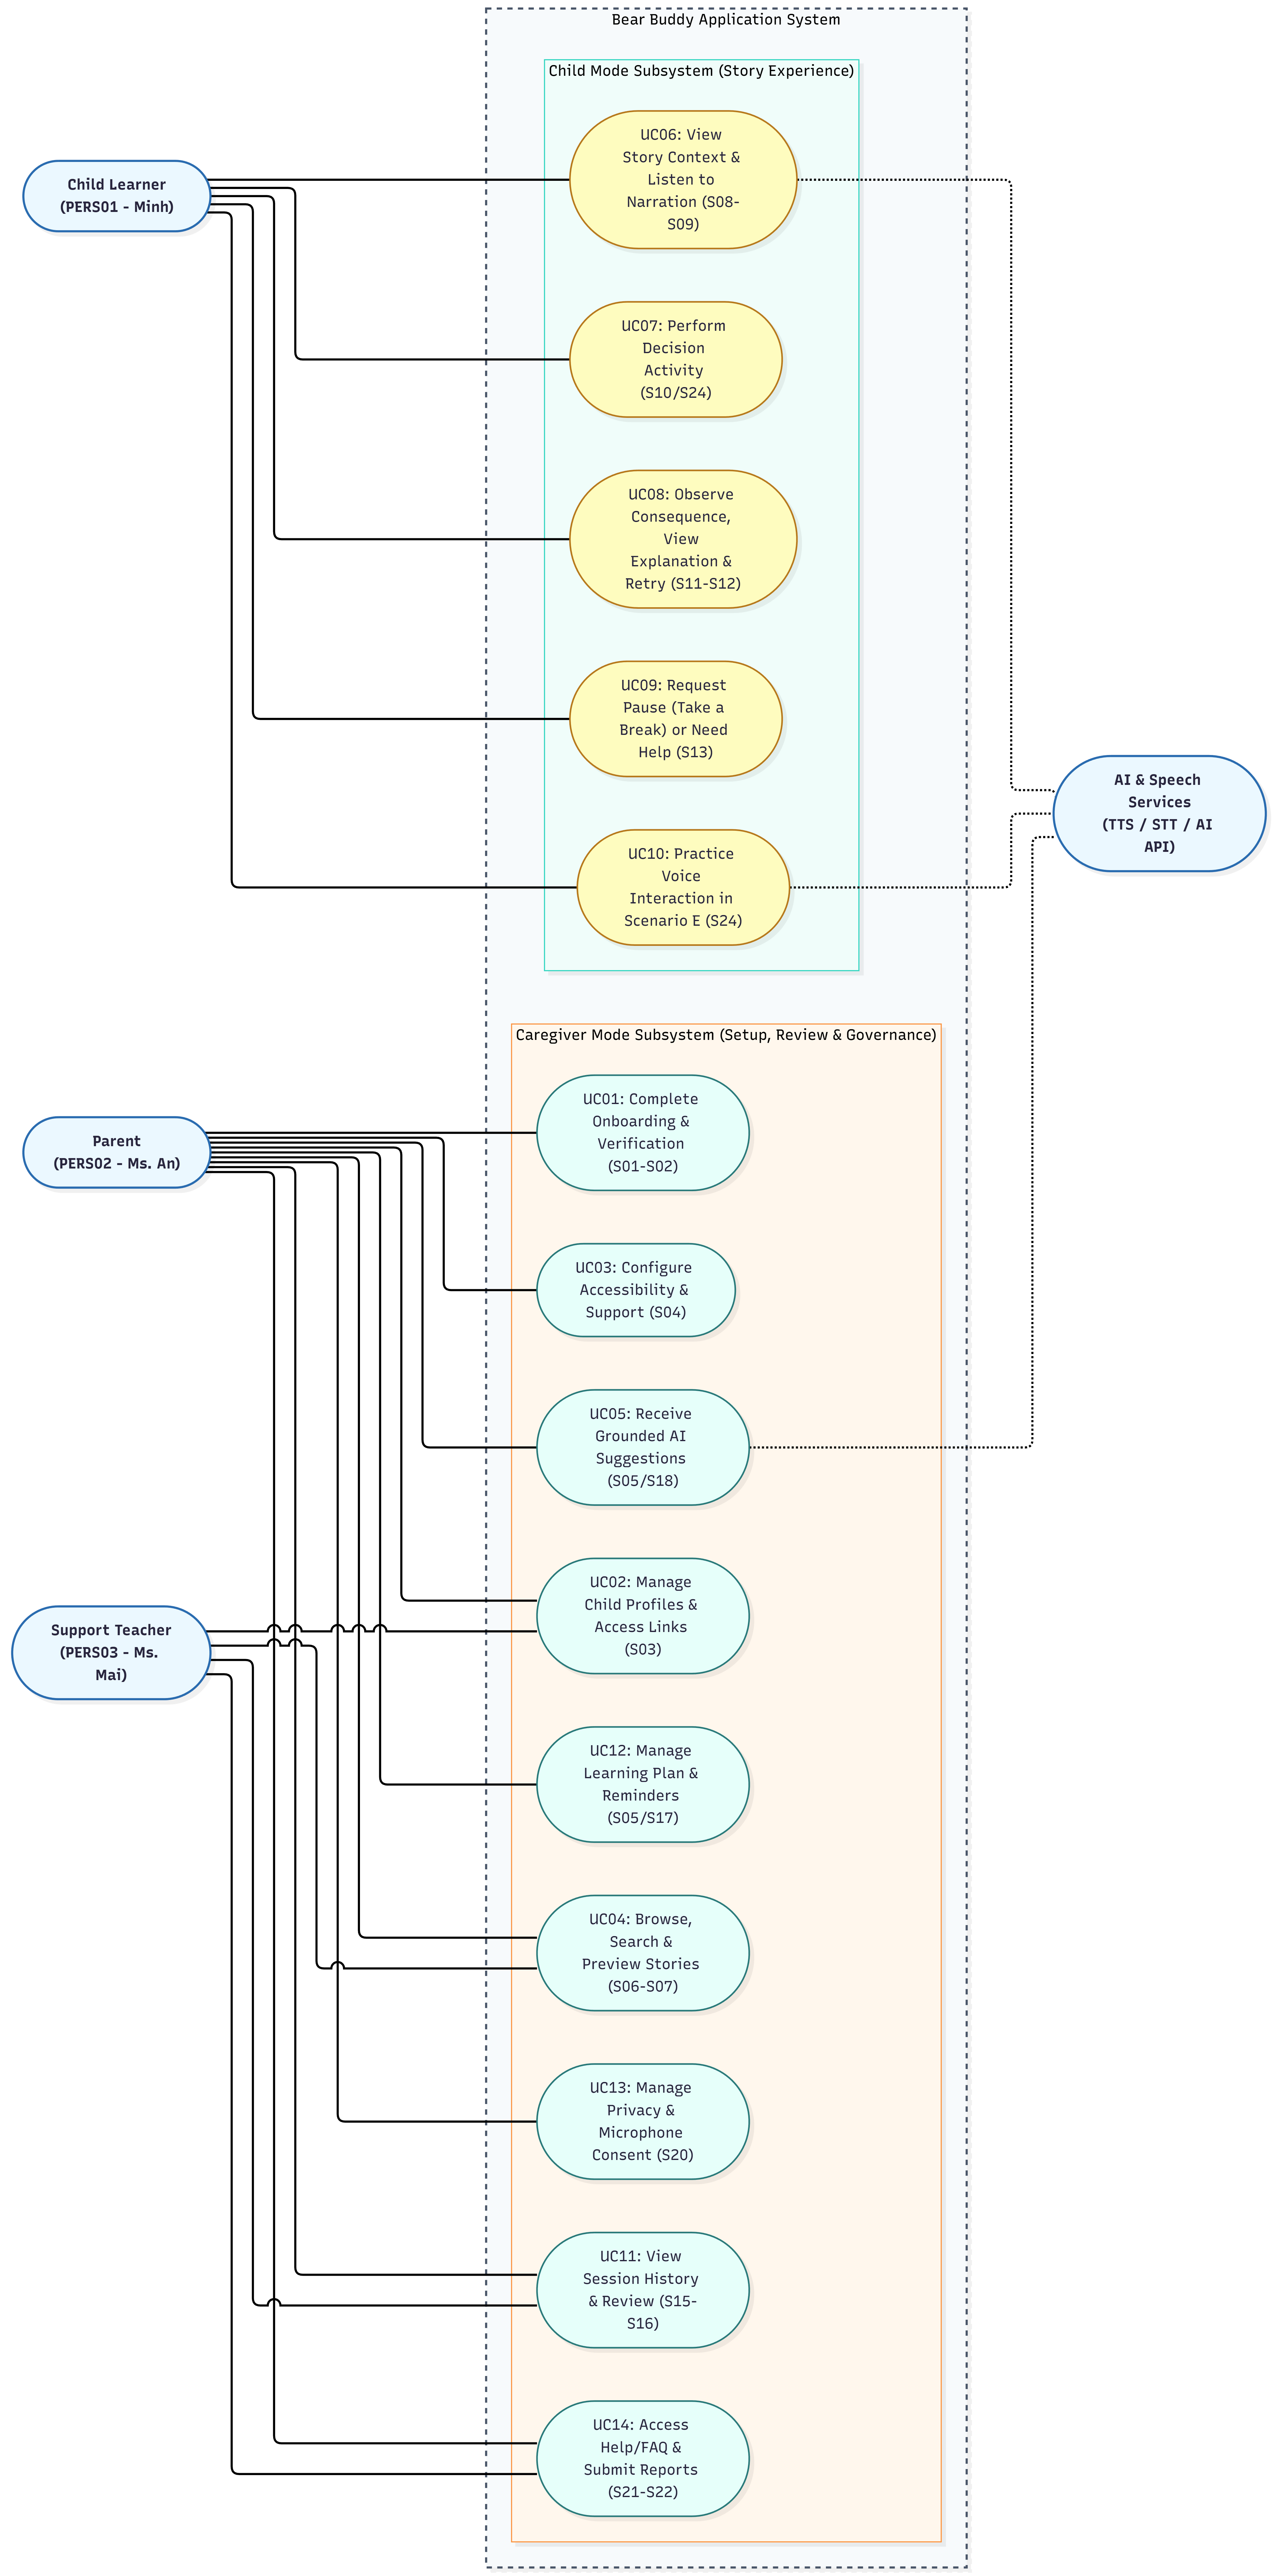
\includegraphics[height=0.86\textheight, keepaspectratio]{figures/use_case_diagram.png}
\caption{Use Case Diagram of the Bear Buddy System}
\label{fig:use_case_diagram}
\end{figure}



\subsection{Use Case Summary Table}


\begin{footnotesize}
\noindent\begin{xltabular}{\textwidth}{|c|p{2.2cm}|X|p{2.0cm}|p{2.4cm}|}
\hline
\textbf{UC ID} & \textbf{Use Case Name} & \textbf{Primary Actor(s)} & \textbf{Linked FRs} & \textbf{Associated Screens (\texttt{S01}–\texttt{S24})} \\ \hline
\endhead
\textbf{UC01} & Complete Onboarding and Caregiver Verification & Parent, Teacher & \texttt{FR01}, \texttt{FR02} & \texttt{S01}, \texttt{S02}, \texttt{S05} \\ \hline
\textbf{UC02} & Manage Child Profiles and Teacher Access Links & Parent & \texttt{FR03}, \texttt{FR04} & \texttt{S03}, \texttt{S05}, \texttt{S20} \\ \hline
\textbf{UC03} & Configure Support and Accessibility Settings & Parent & \texttt{FR03}, \texttt{NFR01}–\texttt{NFR08} & \texttt{S04}, \texttt{S19} \\ \hline
\textbf{UC04} & Browse, Search, and Preview Social Stories & Parent, Teacher & \texttt{FR06}–\texttt{FR09} & \texttt{S05}, \texttt{S06}, \texttt{S07}, \texttt{S23} \\ \hline
\textbf{UC05} & Receive Explainable AI Story Suggestions & Parent & \texttt{FR17}, \texttt{FR25} & \texttt{S18}, \texttt{S07}, \texttt{S23} \\ \hline
\textbf{UC06} & View Story Context and Listen to Narration & Child Learner & \texttt{FR05}, \texttt{FR10}, \texttt{FR11} & \texttt{S08}, \texttt{S09}, \texttt{S14} \\ \hline
\textbf{UC07} & Perform Decision Activity & Child Learner & \texttt{FR12} & \texttt{S10} \\ \hline
\textbf{UC08} & Observe Consequence, View Explanation, and Retry & Child Learner & \texttt{FR13}, \texttt{FR14}, \texttt{FR16} & \texttt{S11}, \texttt{S12}, \texttt{S14} \\ \hline
\textbf{UC09} & Request Pause (Take a Break) or Need Help & Child Learner, Caregiver & \texttt{FR15} & \texttt{S08}–\texttt{S13} \\ \hline
\textbf{UC10} & Practice Voice Interaction in Scenario E & Child Learner & \texttt{FR18}, \texttt{FR25} & \texttt{S24}, \texttt{S10}, \texttt{S23} \\ \hline
\textbf{UC11} & View Session History and Versioned Review & Parent, Teacher & \texttt{FR19}, \texttt{FR20}, \texttt{FR22} & \texttt{S15}, \texttt{S16} \\ \hline
\textbf{UC12} & Manage Learning Plan and Activity Reminders & Parent & \texttt{FR21} & \texttt{S17}, \texttt{S19}, \texttt{S23} \\ \hline
\textbf{UC13} & Manage Privacy, Microphone, and Data Consent & Parent & \texttt{FR23} & \texttt{S20} \\ \hline
\textbf{UC14} & Access Help/FAQ and Submit Feedback/Issue Reports & Parent, Teacher & \texttt{FR24}, \texttt{FR25} & \texttt{S21}, \texttt{S22}, \texttt{S23} \\ \hline
\end{xltabular}
\end{footnotesize}



\subsection{Detailed Use Case Specification Tables}



\subsubsection{UC01 — Complete Onboarding and Caregiver Verification}


\noindent\begin{xltabular}{\textwidth}{|p{4.0cm}|X|}
\hline
\textbf{Specification Field} & \textbf{Details} \\ \hline
\endhead
\textbf{Use Case ID \& Name} & \textbf{UC01 — Complete Onboarding and Caregiver Verification} \\ \hline
\textbf{Primary Actors} & Parent (\texttt{PERS02}), Support Teacher (\texttt{PERS03}) \\ \hline
\textbf{Description} & The adult user reviews the application's purpose, understands the companion role, and authenticates to enter \texttt{Caregiver Mode}. \\ \hline
\textbf{Preconditions} & The application is launched on the mobile device. \\ \hline
\textbf{Postconditions} & Onboarding is completed and the caregiver is granted access to \texttt{Caregiver Home} (\texttt{S05}). \\ \hline
\textbf{Main Flow} & 1. The adult opens the Bear Buddy application. \newline 2. The system displays the \texttt{Introduction} screen (\texttt{S01}) explaining situational preparation, the separation between Caregiver Mode and Child Mode, and the scope of review logs. \newline 3. The user proceeds to \texttt{Account Access} (\texttt{S02}) and signs in or completes the \texttt{Caregiver Gate} PIN/biometric verification. \newline 4. The system validates credentials and opens \texttt{Caregiver Home} (\texttt{S05}). \\ \hline
\textbf{Alternative Flows} & $\bullet$ \textbf{3a. Switching from Child Mode to Caregiver Mode}: The adult triggers the mode switch control and completes the \texttt{Caregiver Gate}; if verification fails or is triggered accidentally by a child's tap, the system remains safely in \texttt{Child Mode} (\texttt{DD31}, \texttt{DD32}). \\ \hline
\end{xltabular}



\subsubsection{UC02 — Manage Child Profiles and Teacher Access Links}


\noindent\begin{xltabular}{\textwidth}{|p{4.0cm}|X|}
\hline
\textbf{Specification Field} & \textbf{Details} \\ \hline
\endhead
\textbf{Use Case ID \& Name} & \textbf{UC02 — Manage Child Profiles and Teacher Access Links} \\ \hline
\textbf{Primary Actor} & Parent (\texttt{PERS02}) \\ \hline
\textbf{Description} & The parent creates or edits a child's profile and manages granting or revoking profile access links for a support teacher (\texttt{PERS03}). \\ \hline
\textbf{Preconditions} & The parent is authenticated in \texttt{Caregiver Mode}. \\ \hline
\textbf{Postconditions} & The child profile and teacher access link permissions are persisted in SQLite. \\ \hline
\textbf{Main Flow} & 1. The parent opens \texttt{Child Profile and Linking} (\texttt{S03}). \newline 2. The parent enters the child's display nickname, avatar, and functional communication/support preferences. \newline 3. The parent optionally generates an access link granting a support teacher (\texttt{PERS03}) permission to view and run sessions for this profile. \newline 4. The system validates inputs, saves the record to SQLite, and sets the profile as active on \texttt{Caregiver Home} (\texttt{S05}). \\ \hline
\textbf{Alternative Flows} & $\bullet$ \textbf{2a. Missing required nickname}: The system highlights the specific field with a friendly inline validation message (\texttt{Invalid Input} - \texttt{S23}) while preserving other entered values. \newline $\bullet$ \textbf{3a. Revoking teacher access}: The parent navigates to \texttt{S20} or \texttt{S03} and revokes the link; the teacher's access is terminated immediately. \\ \hline
\end{xltabular}



\subsubsection{UC03 — Configure Support and Accessibility Settings}


\noindent\begin{xltabular}{\textwidth}{|p{4.0cm}|X|}
\hline
\textbf{Specification Field} & \textbf{Details} \\ \hline
\endhead
\textbf{Use Case ID \& Name} & \textbf{UC03 — Configure Support and Accessibility Settings} \\ \hline
\textbf{Primary Actor} & Parent (\texttt{PERS02}) \\ \hline
\textbf{Description} & The parent customizes font scaling, contrast, narration playback, motion reduction, and interaction modalities tailored to the child's sensory and motor profile. \\ \hline
\textbf{Preconditions} & A valid child profile is selected in \texttt{Caregiver Mode}. \\ \hline
\textbf{Postconditions} & Accessibility settings are saved to the child's profile and applied across all story sessions. \\ \hline
\textbf{Main Flow} & 1. The parent opens \texttt{Accessibility Setup} (\texttt{S04}) during onboarding or from \texttt{Settings} (\texttt{S19}). \newline 2. The parent adjusts the font scale factor (up to $200\%$), toggles auto-narration, sets speech rate, enables Reduce Motion, and configures Scenario E voice participation. \newline 3. The system renders a live preview of the selected settings. \newline 4. The parent saves the configuration to the \texttt{accessibility\_settings} table in SQLite. \\ \hline
\textbf{Alternative Flows} & $\bullet$ \textbf{2a. Reset to Calm Defaults}: The parent selects "Restore Default Settings" to revert all parameters to the baseline sensory-friendly configuration. \\ \hline
\end{xltabular}



\subsubsection{UC04 — Browse, Search, and Preview Social Stories}


\noindent\begin{xltabular}{\textwidth}{|p{4.0cm}|X|}
\hline
\textbf{Specification Field} & \textbf{Details} \\ \hline
\endhead
\textbf{Use Case ID \& Name} & \textbf{UC04 — Browse, Search, and Preview Social Stories} \\ \hline
\textbf{Primary Actors} & Parent (\texttt{PERS02}), Support Teacher (\texttt{PERS03}) \\ \hline
\textbf{Description} & The caregiver searches or filters the story library, inspects learning goals and version metadata, and previews all scenes before starting a session with the child. \\ \hline
\textbf{Preconditions} & The caregiver is in \texttt{Caregiver Mode} with an active child profile selected. \\ \hline
\textbf{Postconditions} & A story is selected and launched into \texttt{Child Mode}. \\ \hline
\textbf{Main Flow} & 1. The caregiver opens \texttt{Story Library} (\texttt{S06}) and browses by category, popular stories, or keyword search. \newline 2. The caregiver selects a story card to open \texttt{Story Details and Preview} (\texttt{S07}). \newline 3. The system displays the social goal, context summary, interaction types, \texttt{story\_version}, and allows the caregiver to step through a full preview of the scenes and explanations. \newline 4. The caregiver taps \texttt{Start with Child} to transition the app into \texttt{Child Mode} (\texttt{S08}/\texttt{S09}). \\ \hline
\textbf{Alternative Flows} & $\bullet$ \textbf{1a. No matching search results}: The system displays the \texttt{Empty Search} state (\texttt{S23}) with a button to clear filters. \newline $\bullet$ \textbf{3a. Content load failure}: The system displays \texttt{Content Load Error} (\texttt{S23}), preserves the active profile context, and provides a \texttt{Retry} button. \\ \hline
\end{xltabular}



\subsubsection{UC05 — Receive Explainable AI Story Suggestions}


\noindent\begin{xltabular}{\textwidth}{|p{4.0cm}|X|}
\hline
\textbf{Specification Field} & \textbf{Details} \\ \hline
\endhead
\textbf{Use Case ID \& Name} & \textbf{UC05 — Receive Explainable AI Story Suggestions} \\ \hline
\textbf{Primary Actors} & Parent (\texttt{PERS02}), AI Recommendation Service \\ \hline
\textbf{Description} & The parent specifies an upcoming situation or learning goal and receives grounded story recommendations from the library accompanied by clear explanations. \\ \hline
\textbf{Preconditions} & The parent is on the \texttt{Parent AI Suggestions} screen (\texttt{S18}). \\ \hline
\textbf{Postconditions} & Recommended stories with explanations are displayed; the parent retains full authority to select or ignore them. \\ \hline
\textbf{Main Flow} & 1. The parent opens \texttt{S18} and selects or enters a situational goal (e.g., preparing for a doctor visit or joining peers at recess). \newline 2. The system verifies AI data consent (\texttt{S20}) and sends an anonymized request to the recommendation module. \newline 3. The system displays matching stories from the library along with a transparent explanation of why each story fits the goal (\texttt{DD39}). \newline 4. The parent taps a recommended story to preview it (\texttt{S07}) or chooses a different story from the library. \\ \hline
\textbf{Alternative Flows} & $\bullet$ \textbf{2a. Device Offline or AI Timeout}: The system displays \texttt{AI Timeout or Unavailable} (\texttt{S23}) and immediately provides deterministic rule-based suggestions from the local SQLite library. \\ \hline
\end{xltabular}



\subsubsection{UC06 — View Story Context and Listen to Narration}


\noindent\begin{xltabular}{\textwidth}{|p{4.0cm}|X|}
\hline
\textbf{Specification Field} & \textbf{Details} \\ \hline
\endhead
\textbf{Use Case ID \& Name} & \textbf{UC06 — View Story Context and Listen to Narration} \\ \hline
\textbf{Primary Actors} & Child Learner (\texttt{PERS01}), Native TTS Service \\ \hline
\textbf{Description} & The child views the illustrated scene, reads short concrete text, and listens to audio narration to understand who is present, what is happening, and which social cues are relevant. \\ \hline
\textbf{Preconditions} & A story session has been launched into \texttt{Child Mode}. \\ \hline
\textbf{Postconditions} & The child receives the situational context (\texttt{Understand}) and is ready for the decision activity. \\ \hline
\textbf{Main Flow} & 1. If this is the child's first session, the system presents the brief \texttt{Child Orientation} screen (\texttt{S08}). \newline 2. The system displays \texttt{Story Context} (\texttt{S09}) with focused character illustration, 1–2 short sentences, and a progress indicator. \newline 3. The system plays the narration via \texttt{SpeechController} according to the profile's audio settings. \newline 4. The child taps \texttt{Replay} to listen again or taps \texttt{Next} to proceed to the activity step. \\ \hline
\textbf{Alternative Flows} & $\bullet$ \textbf{4a. Rapid repeated taps on Replay}: The audio controller stops the active utterance and restarts cleanly from the beginning without overlapping audio streams (\texttt{DD23}). \\ \hline
\end{xltabular}



\subsubsection{UC07 — Perform Decision Activity}


\noindent\begin{xltabular}{\textwidth}{|p{4.0cm}|X|}
\hline
\textbf{Specification Field} & \textbf{Details} \\ \hline
\endhead
\textbf{Use Case ID \& Name} & \textbf{UC07 — Perform Decision Activity} \\ \hline
\textbf{Primary Actor} & Child Learner (\texttt{PERS01}) \\ \hline
\textbf{Description} & The child predicts and selects a behavioral response in the scenario using single-tap interaction on illustrated options. \\ \hline
\textbf{Preconditions} & The child has viewed the story context (\texttt{S09}) and reached \texttt{Decision Activity} (\texttt{S10}). \\ \hline
\textbf{Postconditions} & The child's choice is logged in the session record and the flow advances to \texttt{Consequence} (\texttt{S11}). \\ \hline
\textbf{Main Flow} & 1. The system displays a clear situational prompt and 2 to 3 \texttt{Choice Cards} with distinct illustrations and short labels (\texttt{S10}). \newline 2. The child may tap the speaker icon on any card to hear that option read aloud. \newline 3. The child taps a choice card (or taps cards in sequence 1 $\rightarrow$ 2 $\rightarrow$ 3 for \texttt{Tap-to-Order} activities). \newline 4. The system immediately updates the visual selection state (\texttt{DD24}) and transitions to the \texttt{Consequence} screen (\texttt{S11}). \\ \hline
\textbf{Alternative Flows} & $\bullet$ \textbf{3a. Accidental multi-touch or rapid repeated taps}: The system registers only the first valid touch target and locks duplicate submissions during transition (\texttt{DD29}). \\ \hline
\end{xltabular}



\subsubsection{UC08 — Observe Consequence, View Explanation, and Retry}


\noindent\begin{xltabular}{\textwidth}{|p{4.0cm}|X|}
\hline
\textbf{Specification Field} & \textbf{Details} \\ \hline
\endhead
\textbf{Use Case ID \& Name} & \textbf{UC08 — Observe Consequence, View Explanation, and Retry} \\ \hline
\textbf{Primary Actor} & Child Learner (\texttt{PERS01}) \\ \hline
\textbf{Description} & The child observes how characters in the story react to the chosen action, hears the explanation of why (\texttt{Action} $\rightarrow$ \texttt{Reaction} $\rightarrow$ \texttt{Why}), and chooses whether to replay, retry another option, or continue. \\ \hline
\textbf{Preconditions} & The child has selected an option on \texttt{S10} (or \texttt{S24}). \\ \hline
\textbf{Postconditions} & The child views the explanation and either explores another branch or completes the story at \texttt{S14}. \\ \hline
\textbf{Main Flow} & 1. The system renders \texttt{Consequence} (\texttt{S11}), illustrating the character's specific reaction to the selected action. \newline 2. The system presents \texttt{Explanation and Retry} (\texttt{S12}), explaining why the character reacted that way in this context. \newline 3. The system provides three clear actions: \texttt{Replay} (listen again), \texttt{Try Another Way} (\texttt{Retry}), or \texttt{Next} (continue). \newline 4. Upon completing the final scene, the system displays \texttt{Session End} (\texttt{S14}) acknowledging the child's participation. \\ \hline
\textbf{Alternative Flows} & $\bullet$ \textbf{3a. Child selects \texttt{Try Another Way} (\texttt{Retry})}: The system returns to \texttt{S10} so the child can explore an alternative choice without penalty or negative judgment (\texttt{DD18}). \\ \hline
\end{xltabular}



\subsubsection{UC09 — Request Pause (Take a Break) or Need Help}


\noindent\begin{xltabular}{\textwidth}{|p{4.0cm}|X|}
\hline
\textbf{Specification Field} & \textbf{Details} \\ \hline
\endhead
\textbf{Use Case ID \& Name} & \textbf{UC09 — Request Pause (Take a Break) or Need Help} \\ \hline
\textbf{Primary Actors} & Child Learner (\texttt{PERS01}), Caregiver (\texttt{PERS02}/\texttt{PERS03}) \\ \hline
\textbf{Description} & The child proactively taps \texttt{Pause} (\textit{Take a Break}) or \texttt{Need Help} at any point during a session when feeling tired, overwhelmed, or needing adult support. \\ \hline
\textbf{Preconditions} & An active story session is running in \texttt{Child Mode} (\texttt{S08}–\texttt{S12}, \texttt{S24}). \\ \hline
\textbf{Postconditions} & The session is safely paused at the current step and the event is recorded in the session log. \\ \hline
\textbf{Main Flow} & 1. The child taps the persistent \texttt{Pause} or \texttt{Need Help} button. \newline 2. The system immediately halts all audio playback and opens the calm \texttt{Pause and Help} screen (\texttt{S13}). \newline 3. If \texttt{Need Help} was tapped, the screen displays a concise coaching tip for the accompanying adult. \newline 4. When ready, the child taps \texttt{Resume Story} to return to the exact step, or the adult authenticates to exit to \texttt{Caregiver Mode}. \\ \hline
\textbf{Alternative Flows} & $\bullet$ \textbf{4a. App closed while paused}: The system commits the \texttt{PAUSED} state and \texttt{last\_step\_order} to SQLite so the session can be resumed later (\texttt{S23}). \\ \hline
\end{xltabular}



\subsubsection{UC10 — Practice Voice Interaction in Scenario E}


\noindent\begin{xltabular}{\textwidth}{|p{4.0cm}|X|}
\hline
\textbf{Specification Field} & \textbf{Details} \\ \hline
\endhead
\textbf{Use Case ID \& Name} & \textbf{UC10 — Practice Voice Interaction in Scenario E} \\ \hline
\textbf{Primary Actors} & Child Learner (\texttt{PERS01}), On-Device Speech Recognition Service \\ \hline
\textbf{Description} & In Scenario E, when voice practice is enabled, the child practices speaking a short functional social phrase or selects a parallel touch card alternative. \\ \hline
\textbf{Preconditions} & Voice interaction is enabled for the profile and the story reaches Scenario E (\texttt{S24}). \\ \hline
\textbf{Postconditions} & The child's response (via speech or touch) is confirmed and the story advances to \texttt{Consequence} (\texttt{S11}). \\ \hline
\textbf{Main Flow} & 1. The system displays \texttt{Voice Interaction Scenario E} (\texttt{S24}) with the model phrase prompt (e.g., \textit{"Can I play too?"}), a \texttt{Listen to Model} button, a central \texttt{Tap to Speak} button, and parallel illustrated touch cards. \newline 2. The child taps \texttt{Tap to Speak} and says the short phrase. \newline 3. The voice controller matches the recognized transcript against target keywords for the scenario. \newline 4. Upon keyword match, the system confirms the choice and transitions to \texttt{Consequence} (\texttt{S11}). \\ \hline
\textbf{Alternative Flows} & $\bullet$ \textbf{1a. Child prefers touch or Microphone Denied (\texttt{Microphone Denied})}: The child taps the illustrated choice card directly on \texttt{S24} to complete the step without speaking (\texttt{DD36}). \newline $\bullet$ \textbf{3a. Unclear audio (\texttt{Speech Not Recognized})}: The system displays \textit{"Not heard clearly. Choose a picture or try again"} (\texttt{S23}) without grading pronunciation as wrong. \\ \hline
\end{xltabular}



\subsubsection{UC11 — View Session History and Versioned Review}


\noindent\begin{xltabular}{\textwidth}{|p{4.0cm}|X|}
\hline
\textbf{Specification Field} & \textbf{Details} \\ \hline
\endhead
\textbf{Use Case ID \& Name} & \textbf{UC11 — View Session History and Versioned Review} \\ \hline
\textbf{Primary Actors} & Parent (\texttt{PERS02}), Support Teacher (\texttt{PERS03}) \\ \hline
\textbf{Description} & The caregiver reviews the list of past sessions for the selected child profile and inspects the exact sequence of choices and explanations experienced. \\ \hline
\textbf{Preconditions} & The caregiver is authenticated and authorized for the selected child profile. \\ \hline
\textbf{Postconditions} & Version-accurate session review records are displayed descriptively. \\ \hline
\textbf{Main Flow} & 1. The caregiver opens \texttt{Session History} (\texttt{S15}) to view chronological sessions for the active child profile. \newline 2. The caregiver selects a session to open \texttt{Session Review} (\texttt{S16}). \newline 3. The system queries SQLite joining the exact \texttt{story\_version\_id} and displays the story title, version code, timestamp, choices selected, explanations viewed, and \texttt{Replay}/\texttt{Retry}/\texttt{Pause}/\texttt{Help} counts. \newline 4. The caregiver records optional reflection notes and proceeds to plan the next activity (\texttt{S17}). \\ \hline
\textbf{Alternative Flows} & $\bullet$ \textbf{1a. No sessions recorded yet}: The system displays the \texttt{Empty History} state (\texttt{S23}) with a direct link to the Story Library. \\ \hline
\end{xltabular}



\subsubsection{UC12 — Manage Learning Plan and Activity Reminders}


\noindent\begin{xltabular}{\textwidth}{|p{4.0cm}|X|}
\hline
\textbf{Specification Field} & \textbf{Details} \\ \hline
\endhead
\textbf{Use Case ID \& Name} & \textbf{UC12 — Manage Learning Plan and Activity Reminders} \\ \hline
\textbf{Primary Actor} & Parent (\texttt{PERS02}) \\ \hline
\textbf{Description} & The parent selects upcoming stories for the child's learning plan and configures local reminder notifications. \\ \hline
\textbf{Preconditions} & The parent is in \texttt{Caregiver Mode}. \\ \hline
\textbf{Postconditions} & Planned stories and local notification schedules are saved. \\ \hline
\textbf{Main Flow} & 1. The parent opens \texttt{Learning Plan} (\texttt{S17}) from Caregiver Home or after reviewing a session. \newline 2. The parent adds target stories to the child's plan. \newline 3. The parent enables reminders and selects preferred days and time (\texttt{S17}/\texttt{S19}). \newline 4. The system requests OS notification permission (if needed) and schedules local reminders via \texttt{ReminderService}. \\ \hline
\textbf{Alternative Flows} & $\bullet$ \textbf{4a. OS Notifications Disabled (\texttt{Notification Disabled})}: The system saves the learning plan in SQLite, indicates that reminders are off on \texttt{S19}/\texttt{S23}, and never blocks child story access. \\ \hline
\end{xltabular}



\subsubsection{UC13 — Manage Privacy, Microphone, and Data Consent}


\noindent\begin{xltabular}{\textwidth}{|p{4.0cm}|X|}
\hline
\textbf{Specification Field} & \textbf{Details} \\ \hline
\endhead
\textbf{Use Case ID \& Name} & \textbf{UC13 — Manage Privacy, Microphone, and Data Consent} \\ \hline
\textbf{Primary Actor} & Parent (\texttt{PERS02}) \\ \hline
\textbf{Description} & The parent manages data collection consents, microphone usage, AI history sharing, teacher links, and data deletion. \\ \hline
\textbf{Preconditions} & The parent is authenticated in \texttt{Caregiver Mode}. \\ \hline
\textbf{Postconditions} & Privacy preferences are updated immediately and logged in \texttt{consent\_audit\_logs}. \\ \hline
\textbf{Main Flow} & 1. The parent opens \texttt{Privacy and Access} (\texttt{S20}). \newline 2. The system displays current states for Microphone permission (Scenario E), AI history usage consent, and active teacher profile links. \newline 3. The parent toggles permissions or triggers session history deletion. \newline 4. The system applies changes immediately and records an audit entry. \\ \hline
\textbf{Alternative Flows} & $\bullet$ \textbf{3a. Delete entire child profile}: The system requires explicit two-step confirmation before cascading deletion of the profile and its session records in SQLite. \\ \hline
\end{xltabular}



\subsubsection{UC14 — Access Help/FAQ and Submit Feedback/Issue Reports}


\noindent\begin{xltabular}{\textwidth}{|p{4.0cm}|X|}
\hline
\textbf{Specification Field} & \textbf{Details} \\ \hline
\endhead
\textbf{Use Case ID \& Name} & \textbf{UC14 — Access Help/FAQ and Submit Feedback/Issue Reports} \\ \hline
\textbf{Primary Actors} & Parent (\texttt{PERS02}), Support Teacher (\texttt{PERS03}) \\ \hline
\textbf{Description} & The caregiver consults user guides and FAQs or submits an issue report / content feedback. \\ \hline
\textbf{Preconditions} & The caregiver is in \texttt{Caregiver Mode}. \\ \hline
\textbf{Postconditions} & Help content is displayed or the feedback report is queued/submitted. \\ \hline
\textbf{Main Flow} & 1. The caregiver opens \texttt{Help FAQ and Contact} (\texttt{S21}) to review companion guidance and social story principles. \newline 2. To report an issue, the caregiver opens \texttt{Feedback and Issue Report} (\texttt{S22}). \newline 3. The caregiver enters feedback text, chooses whether to attach anonymized \texttt{story\_version}/diagnostic metadata, and taps Submit. \newline 4. The system confirms submission (\texttt{Feedback Submission} - \texttt{S23}). \\ \hline
\textbf{Alternative Flows} & $\bullet$ \textbf{4a. Device Offline during submission}: The system stores the report in the local SQLite queue (\texttt{Save or Sync Pending} - \texttt{S23}) for retry when connectivity returns. \\ \hline
\end{xltabular}



\section{Context Diagram and Data Flow Diagram}



\subsection{Context Diagram}


The Context Diagram represents \textbf{Bear Buddy} as a single central process (\texttt{0.0 Bear Buddy Application System}) to establish the system boundary and external data exchanges.


\begin{figure}[htbp]
\centering
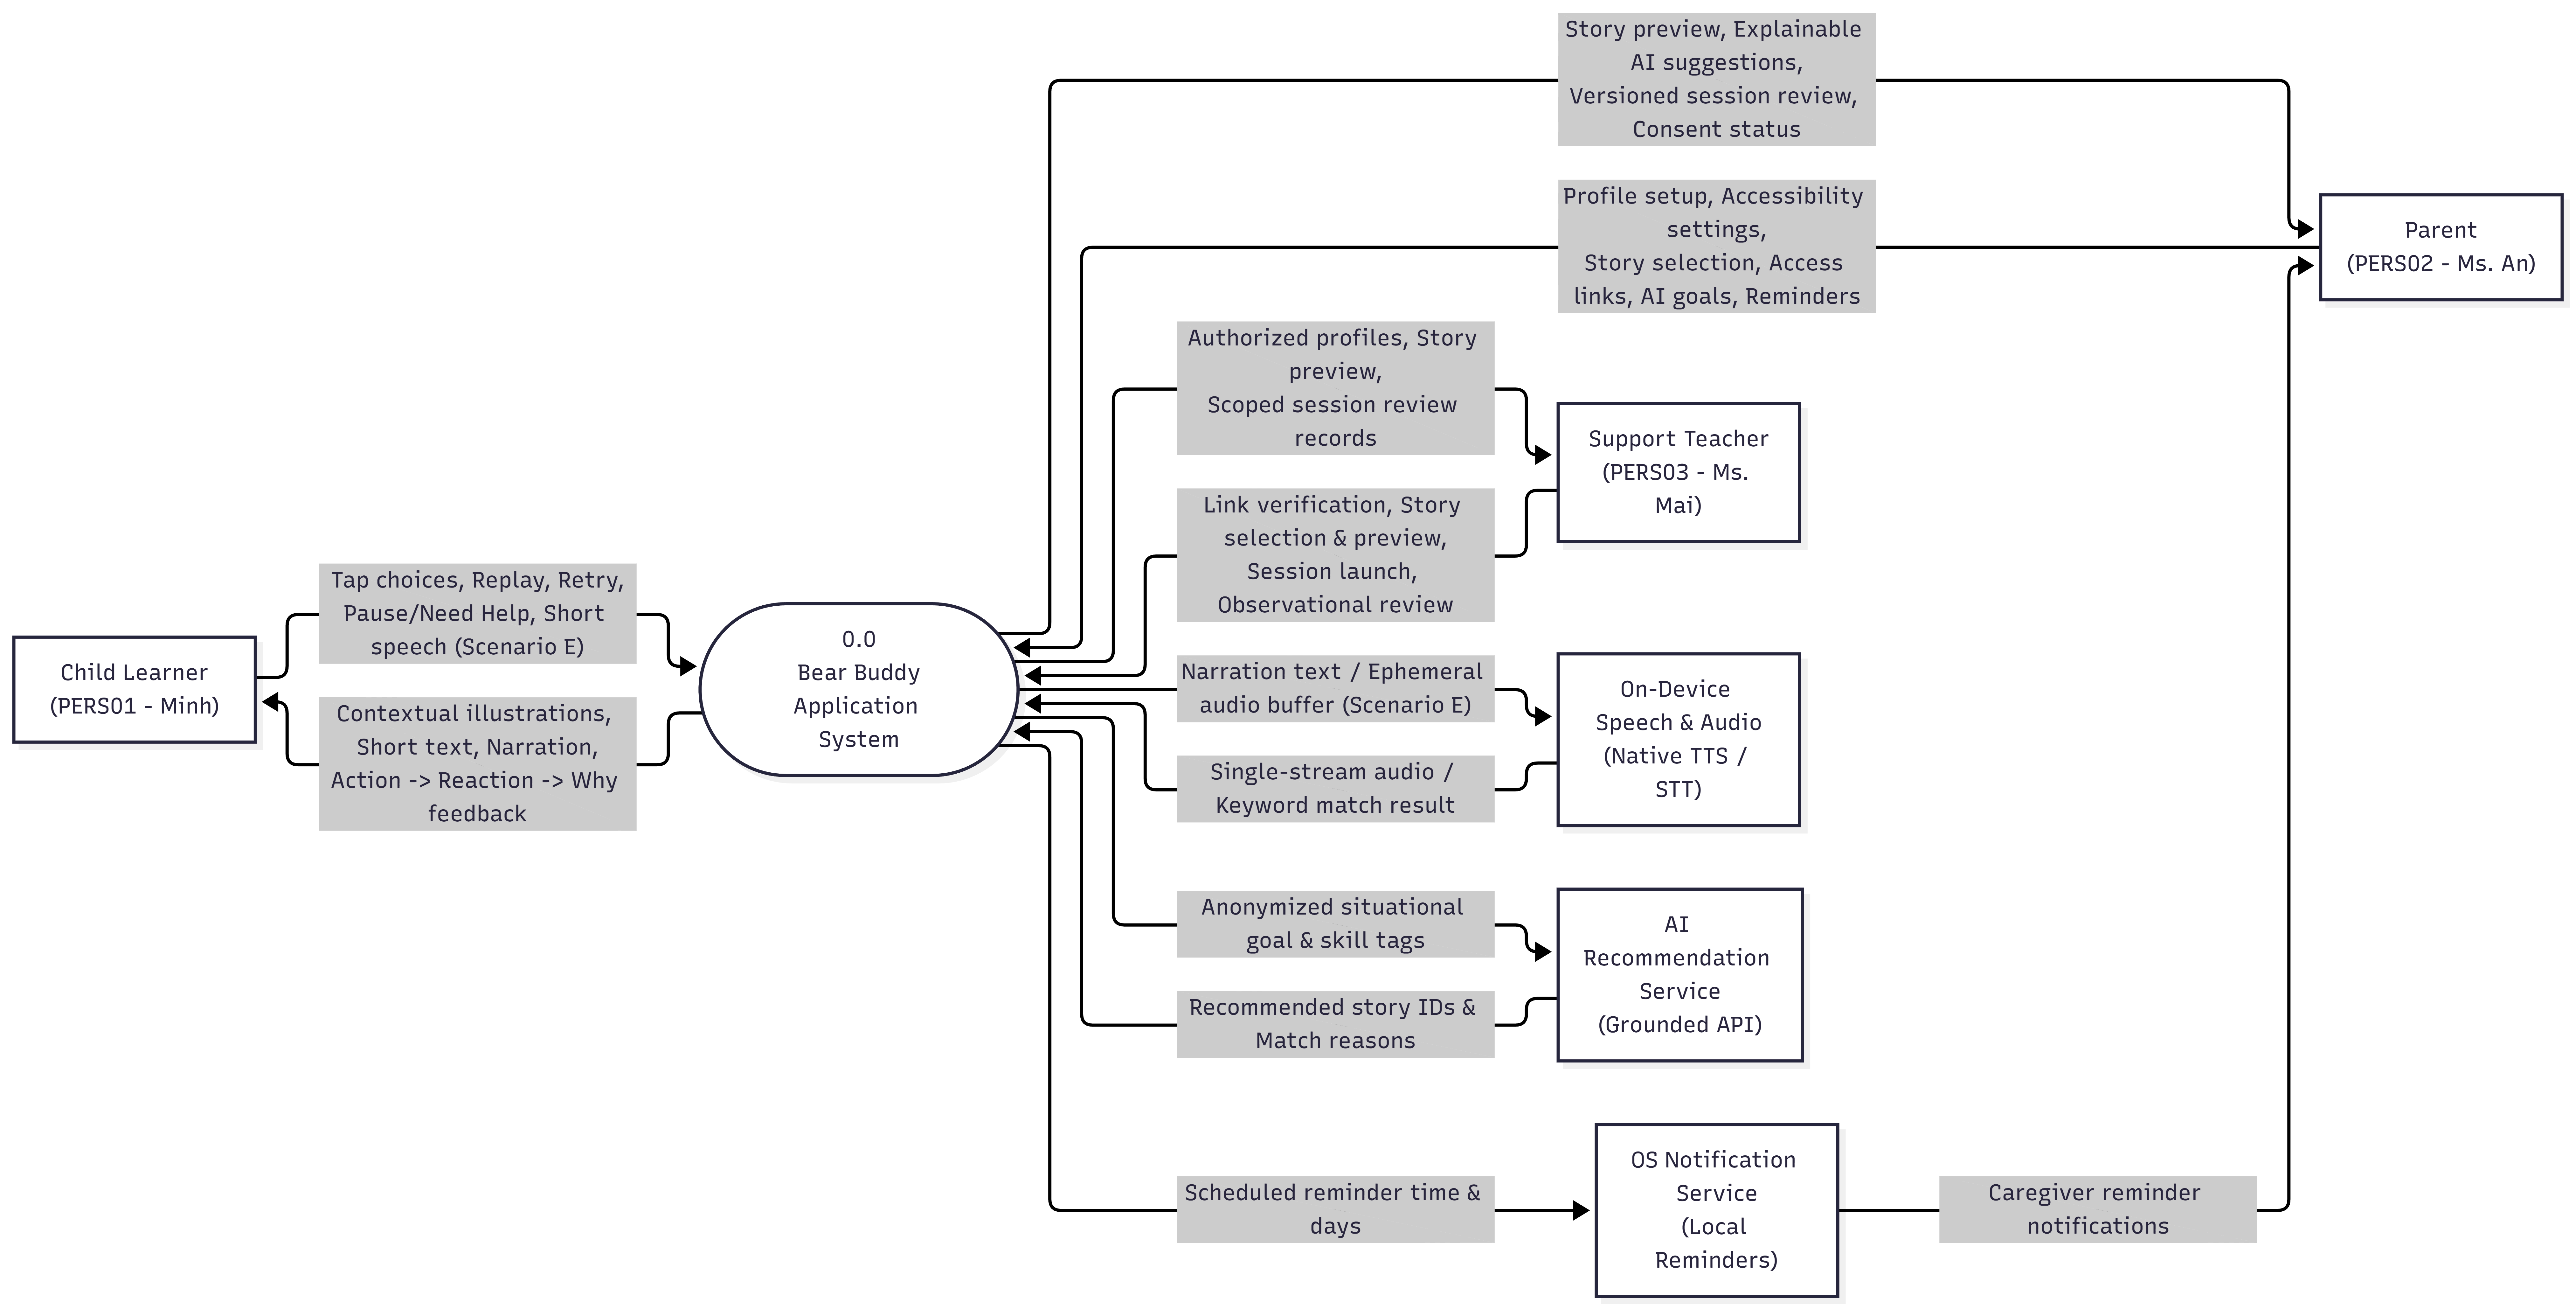
\includegraphics[width=0.92\textwidth]{figures/context_diagram.png}
\caption{Context Diagram of the Bear Buddy System}
\label{fig:context_diagram}
\end{figure}



\subsection{Level 0 Data Flow Diagram (DFD Level 0)}


The Level 0 Data Flow Diagram decomposes Bear Buddy into \textbf{6 core processes} and \textbf{5 local SQLite data stores}, reflecting the strict boundary between child-facing learning processes and caregiver management processes:

\begin{itemize}
  \item \textbf{Core Processes}:
  \item \texttt{1.0 Profile, Role Access \& Accessibility Management}: Handles Caregiver Gate verification, child profiles, teacher access links, accessibility settings, and privacy consents (\texttt{S01}–\texttt{S04}, \texttt{S19}, \texttt{S20}).
  \item \texttt{2.0 Versioned Story Library, Search \& Preview}: Queries stories by category/keyword, tracks \texttt{story\_version}, and renders caregiver previews (\texttt{S05}–\texttt{S07}).
  \item \texttt{3.0 Interactive Story Engine \& Multimodal Player (Child Mode)}: Orchestrates the child learning loop, single-stream narration, touch choices, \texttt{Action} $\rightarrow$ \texttt{Reaction} $\rightarrow$ \texttt{Why} presentation, \texttt{Replay}, \texttt{Retry}, \texttt{Pause}, and \texttt{Need Help} (\texttt{S08}–\texttt{S14}).
  \item \texttt{4.0 Scenario E Voice Processing \& Touch Fallback}: Manages bounded phrase practice on \texttt{S24}, checks microphone consent, matches keywords via STT, and guarantees an immediate touch-card fallback.
  \item \texttt{5.0 Session Logging, Versioned Review \& Learning Plan}: Records interaction events pinned to \texttt{story\_version}, generates descriptive caregiver reviews, and schedules reminders (\texttt{S15}–\texttt{S17}).
  \item \texttt{6.0 Explainable AI Suggestions, Help \& Feedback}: Processes grounded AI story recommendations (\texttt{S18}), FAQ lookup, and issue reporting (\texttt{S21}–\texttt{S23}).
  \item \textbf{Internal SQLite Data Stores}:
  \item \texttt{D1: Child Profiles \& Access Links}: Stores caregiver accounts, child profiles, and parent–teacher access link permissions.
  \item \texttt{D2: Accessibility \& Privacy Settings}: Stores font scaling, contrast, audio, motion reduction, and microphone/AI consent states.
  \item \texttt{D3: Versioned Story Library}: Stores stories, immutable \texttt{story\_version} metadata, scene steps, choices, and explanations.
  \item \texttt{D4: Session Logs \& Review Records}: Stores session metadata and chronological interaction events linked to \texttt{story\_version}.
  \item \texttt{D5: Learning Plans, Reminders \& Feedback Queue}: Stores planned stories, reminder schedules, and pending feedback reports.
\end{itemize}



\begin{figure}[htbp]
\centering
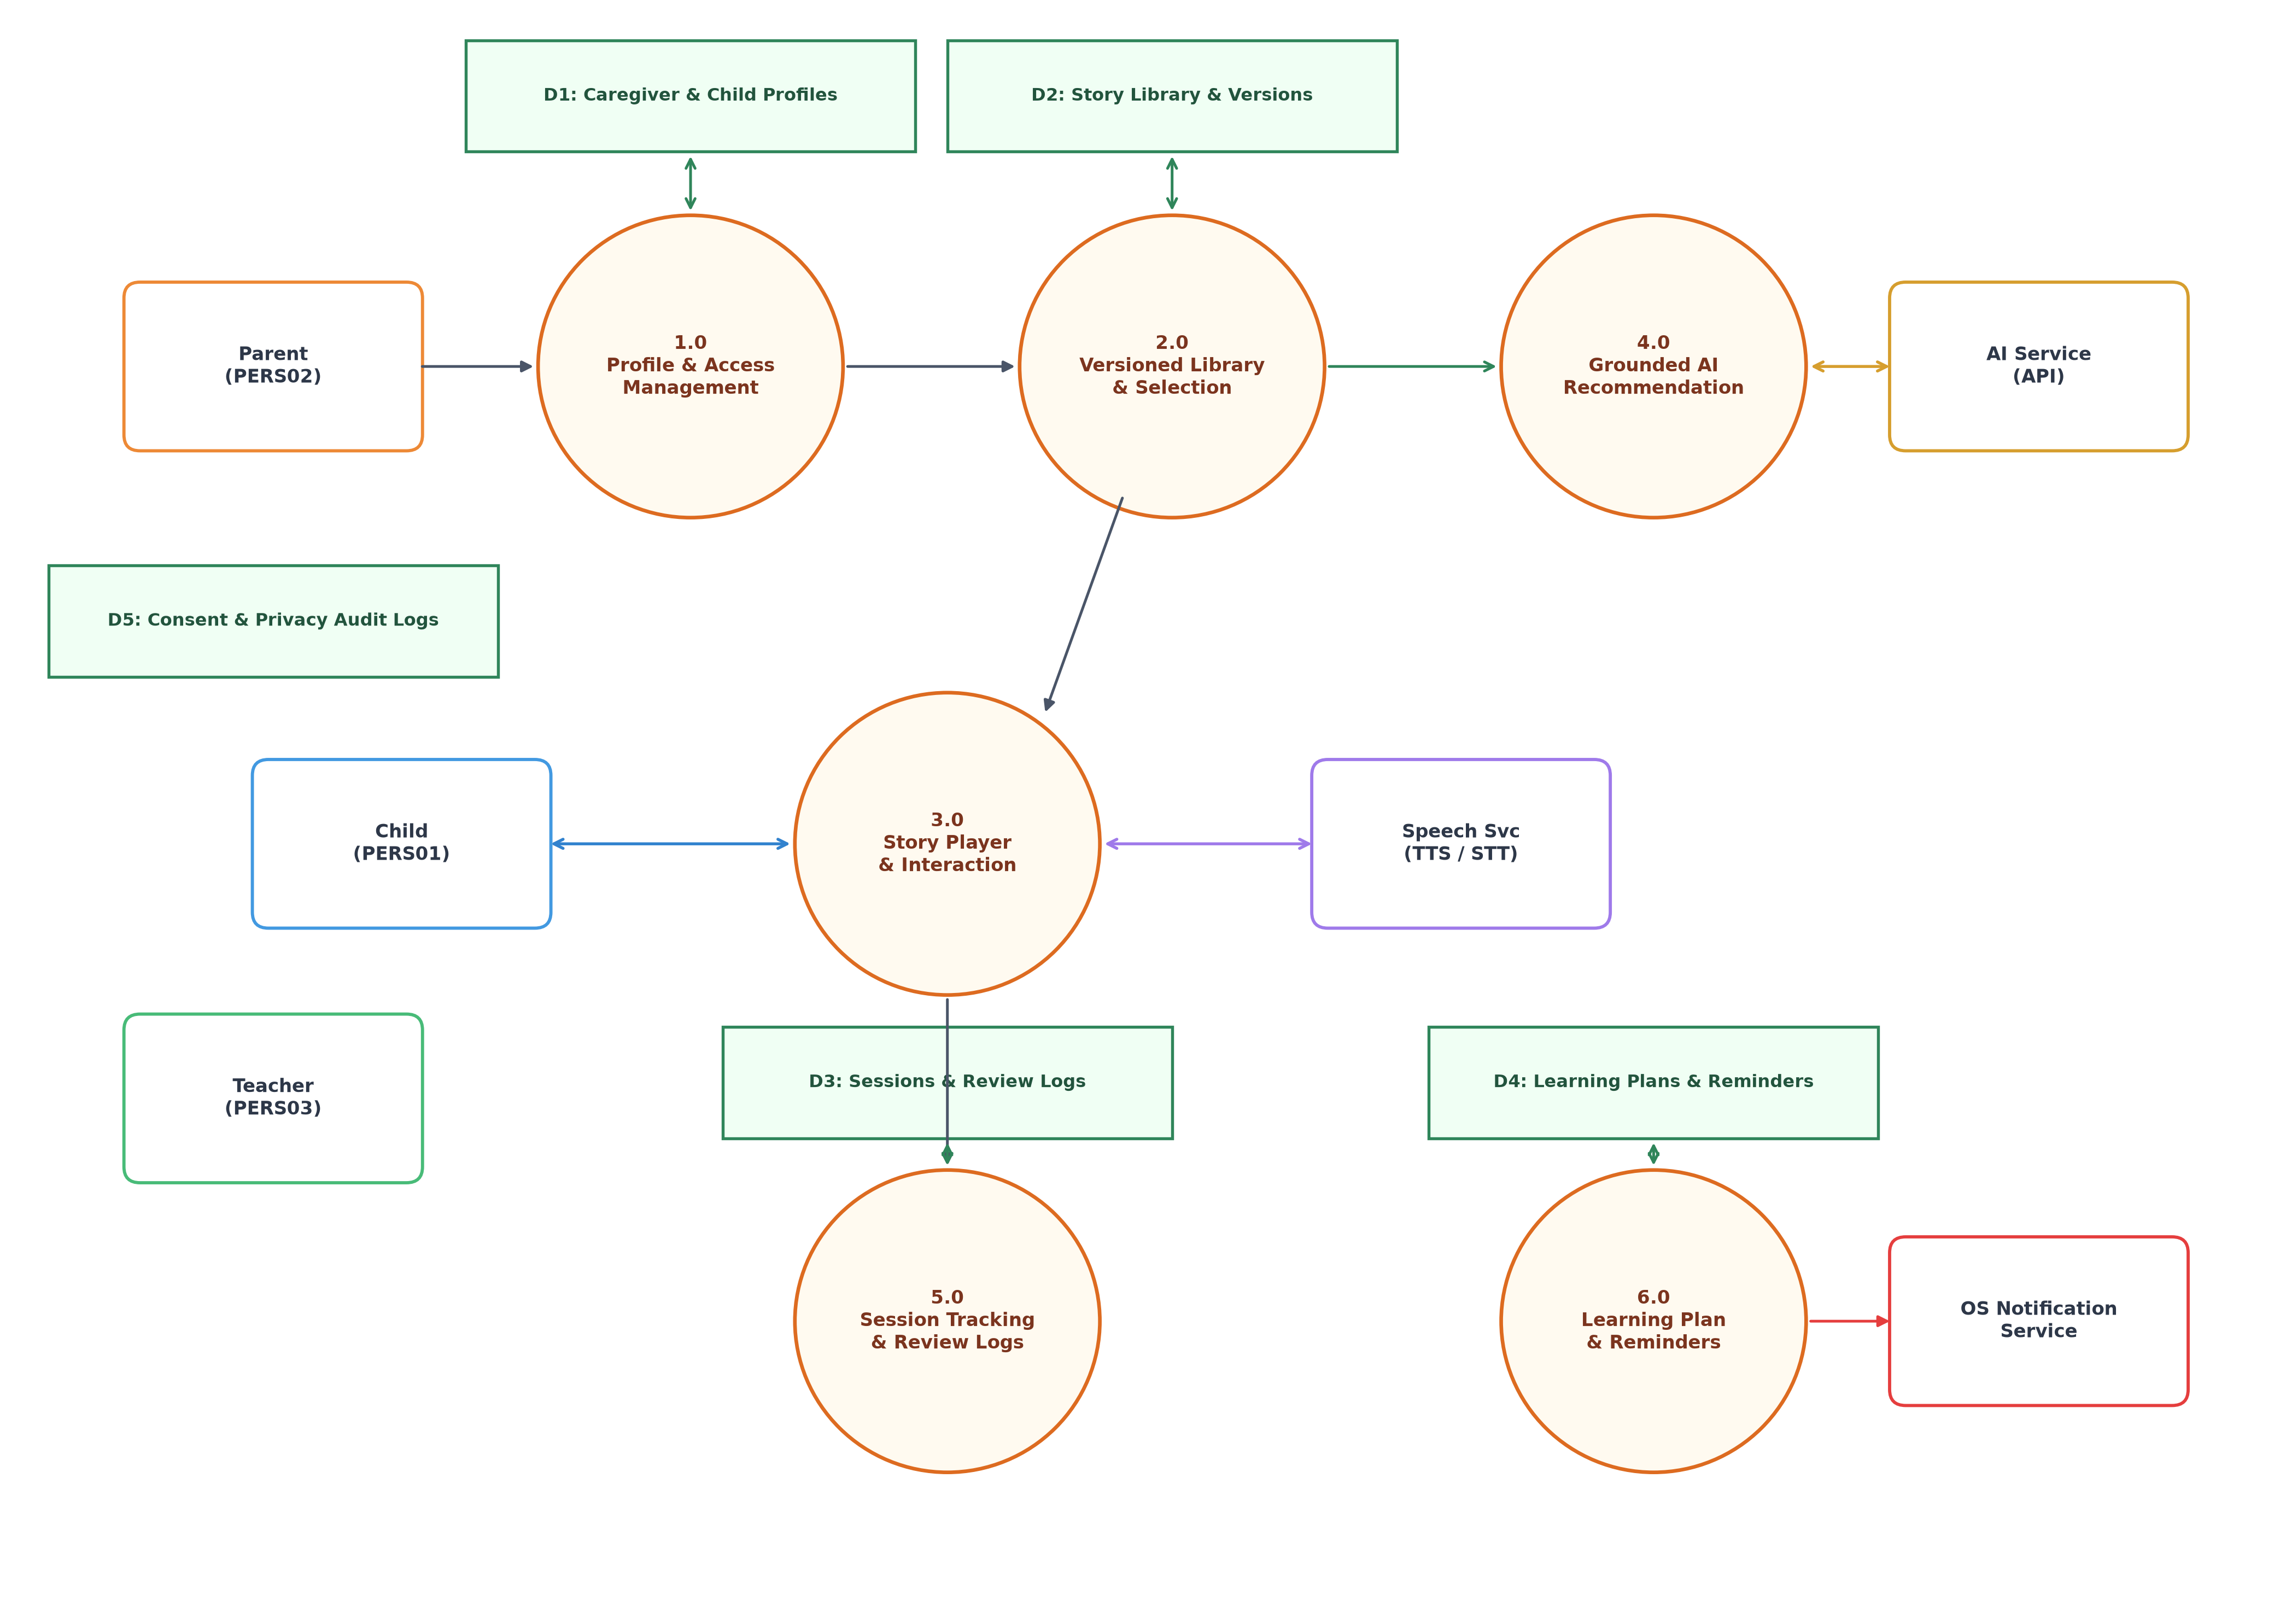
\includegraphics[width=0.95\textwidth]{figures/dfd_level_0.png}
\caption{Level 0 Data Flow Diagram of the Bear Buddy System}
\label{fig:dfd_level_0}
\end{figure}



\subsection{Architectural Observations on System Data Flows}


\begin{enumerate}
  \item \textbf{Strict Separation of Child and Caregiver Data Flows}: The Child Learner (\texttt{PERS01}) interacts exclusively with Processes \texttt{3.0} and \texttt{4.0}. All configuration (\texttt{1.0}), content selection (\texttt{2.0}), historical review (\texttt{5.0}), and AI consultation (\texttt{6.0}) remain isolated within caregiver-authenticated processes.
  \item \textbf{Version-Pinned Historical Integrity (\texttt{story\_version}) across \texttt{D3} and \texttt{D4}}: When Process \texttt{5.0} renders a Session Review for a parent or teacher, it joins the interaction log in \texttt{D4} with the immutable \texttt{story\_version} in \texttt{D3}, guaranteeing that adults see the exact wording and explanation the child experienced during that session.
  \item \textbf{Consent-Gated AI and Voice Execution via \texttt{D2}}: Both Process \texttt{4.0} (Scenario E Voice) and Process \texttt{6.0} (Parent AI Suggestions) must verify explicit permission flags in \texttt{D2: Accessibility \& Privacy} before invoking external or hardware services, while maintaining deterministic local fallbacks from \texttt{D3}.
\end{enumerate}


% Chapter 4: Story Content and Interaction Design
\chapter{Story Content and Interaction Design}


This chapter translates the theoretical foundation of Social Stories from Section 2.2, the multimodal learning principles from Section 2.3, and the UX reasoning framework (\texttt{P1}–\texttt{P11}, \texttt{DD1}–\texttt{DD40}) from Section 5.1 into the concrete story content architecture, interaction modality selection, formal specification of \textbf{Scenario E}, and non-punitive feedback rules for \textbf{Bear Buddy}.


\section{Situation Library Categorization}


The Bear Buddy story library is organized around everyday social situations that children encounter at home, at school, or in community settings. Structuring the library into clear situational themes enables parents (\texttt{PERS02}) and teachers (\texttt{PERS03}) to quickly locate preparatory content before an upcoming real-world event (\texttt{UN07}).


\subsection{Four Core Situational Categories}


\noindent\begin{xltabular}{\textwidth}{|p{2.0cm}|p{3.2cm}|X|p{2.8cm}|}
\hline
\textbf{Category Code} & \textbf{Category Name} & \textbf{Social Preparation Goal} & \textbf{Representative Stories in Scope} \\ \hline
\endhead
\textbf{CAT01} & \textbf{Waiting and Shared Routines} & Helps the child recognize cues that an activity requires taking turns or sharing space, understand what to do while waiting, and know when their turn arrives. & $\bullet$ \textit{Waiting for a Turn on the Slide} \newline $\bullet$ \textit{Quiet Reading Time in the Classroom} \newline $\bullet$ \textit{Lining Up to Wash Hands} \\ \hline
\textbf{CAT02} & \textbf{Peer Entry and Social Play} & Helps the child observe what peers are doing, identify an appropriate moment to approach, ask or signal to join play, and respond when peers agree or are busy. & $\bullet$ \textit{Saying Hello to a New Classmate} \newline $\bullet$ \textit{Asking to Join a Ball Game} \newline $\bullet$ \textit{When a Request to Play Is Not Accepted Yet} \\ \hline
\textbf{CAT03} & \textbf{Needs Expression and Help-Seeking} & Helps the child recognize when a task is difficult or sensory input is overwhelming, locate a trusted adult/peer, and express a need for help or a break via touch, picture card, or short phrase. & $\bullet$ \textit{Asking a Teacher or Parent to Open a Box} \newline $\bullet$ \textit{Telling an Adult When It Is Too Loud} \newline $\bullet$ \textit{Practicing Short Help-Seeking Phrases (Scenario E)} \\ \hline
\textbf{CAT04} & \textbf{Preparing for Novel Events and Transitions} & Helps the child anticipate step-by-step sequences, sensory sensations (sounds, touch), and adult support before visiting a new place or experiencing a schedule change. & $\bullet$ \textit{Visiting the Doctor with Mom} \newline $\bullet$ \textit{Getting a Haircut} \newline $\bullet$ \textit{Moving to a New Classroom Activity} \\ \hline
\end{xltabular}



\subsection{Standardized Metadata, Versioning, and Transparent Popularity Rules}


To satisfy the content versioning requirements in Section 2.2.3 and clarify the \textit{"Most popular social stories"} criteria from Section 1.4.2, every story in the library is governed by standardized metadata:

\begin{itemize}
  \item \textbf{Identifier and Immutable Version (\texttt{story\_id}, \texttt{story\_version})}: Each published release carries an explicit version code (e.g., \texttt{ST\_JOIN\_PLAY\_v1.2}), recording the content author, special education reviewer, media asset sources, and publication timestamp. Whenever an explanation or decision branch is modified, the system creates a new \texttt{story\_version} rather than overwriting historical records.
  \item \textbf{Target Support Metadata}: Specifies the primary interaction modalities used, total scene count, whether an optional Scenario E voice step is included, and preparatory guidance for the caregiver on the \texttt{Story Details} screen (\texttt{S07}).
  \item \textbf{Transparent Rules for "Most Popular Social Stories"}:
  \item \textit{With Real Operational Data}: Popularity is defined transparently as the \textit{total number of completed sessions over the trailing 30-day window}.
  \item \textit{During Initial Deployment / Demo Seed}: Featured items are explicitly badged as \textbf{\texttt{[Sample Featured Story]}} (\texttt{[Demo Seed]}) rather than displaying fabricated usage numbers, accompanied by a reminder that caregivers should choose stories based on the child's current situational need rather than general popularity (\texttt{S06}).
\end{itemize}



\section{Standard Structure of a Bear Buddy Story}


A Bear Buddy story combines the informational structure of Carol Gray's Social Stories (10.4 Criteria) with a predictable interactive sequence (\texttt{DD2}: \texttt{Scene} $\rightarrow$ \texttt{Decision} $\rightarrow$ \texttt{Consequence} $\rightarrow$ \texttt{Explanation} $\rightarrow$ \texttt{Next}). This structure ensures the child always receives sufficient social context before making a decision (\texttt{UN01}, \texttt{DD13}).


\subsection{Five Structural Stages of a Standard Story}



\begin{figure}[htbp]
\centering
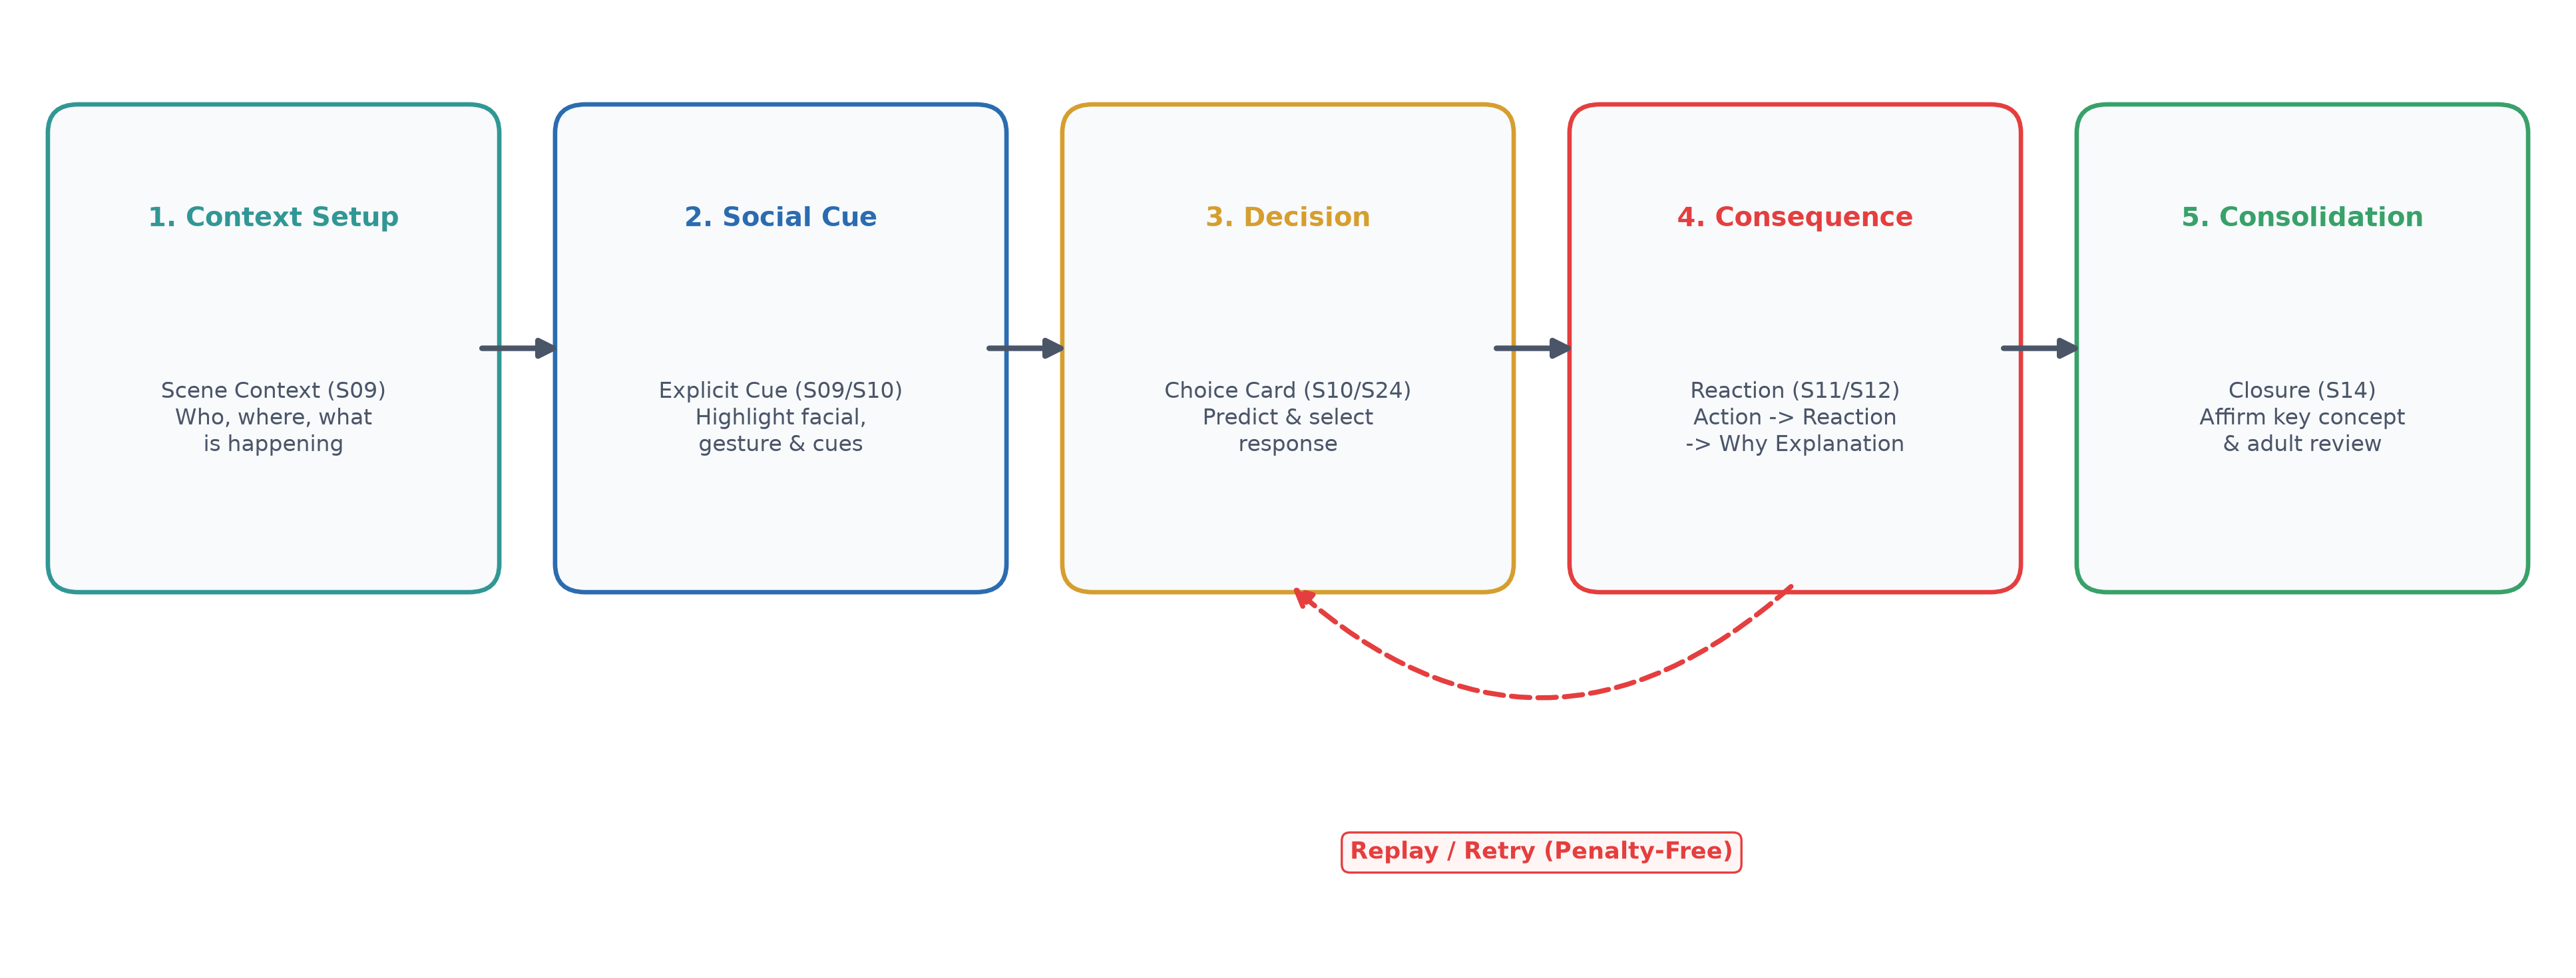
\includegraphics[width=0.95\textwidth]{figures/story_five_stages.png}
\caption{The Five Structural Stages of a Standard Bear Buddy Story}
\label{fig:story_five_stages}
\end{figure}


\begin{enumerate}
  \item \textbf{Stage 1 — Context Setup (Screen \texttt{S09})}:
\end{enumerate}
\begin{itemize}
  \item \textbf{Purpose}: Introduces the characters (e.g., the child character and Bear Buddy), the physical setting (classroom, playground, clinic), and the ongoing activity.
  \item \textbf{Sentence Functions}: Uses concrete \textit{Descriptive} sentences paired with observable, evidence-based \textit{Perspective} sentences.
\end{itemize}
\begin{enumerate}
  \item \textbf{Stage 2 — Explicit Social Cue Presentation (Screens \texttt{S09} / \texttt{S10})}:
\end{enumerate}
\begin{itemize}
  \item \textbf{Purpose}: Implements the core principle \textit{Make the implicit explicit} (\texttt{P3}, \texttt{DD14}). Instead of assuming the child will infer meaning from a small facial expression, the visual highlight and narration explicitly point out the relevant cue (e.g., \textit{"Two friends are rolling a red ball and smiling. They are looking at the ball, so they might not know I want to play yet"}).
\end{itemize}
\begin{enumerate}
  \item \textbf{Stage 3 — Decision Activity (Screen \texttt{S10} or \texttt{S24})}:
\end{enumerate}
\begin{itemize}
  \item \textbf{Purpose}: Presents a single focused situational question (e.g., \textit{"What can I do so my friends know I want to play with them?"}) accompanied by concrete illustrated action choices.
\end{itemize}
\begin{enumerate}
  \item \textbf{Stage 4 — Consequence and Why Explanation (Screens \texttt{S11} \& \texttt{S12})}:
\end{enumerate}
\begin{itemize}
  \item \textbf{Purpose}: Explicitly models the causal chain \textbf{\texttt{Action} $\rightarrow$ \texttt{Reaction} $\rightarrow$ \texttt{Why}} (\texttt{DD15}, \texttt{DD16}):
  \item \textbf{Action (Selected Choice)}: Briefly restates the action the child selected.
  \item \textbf{Reaction (Scenario Outcome)}: Illustrates and describes how the other characters in this specific scenario respond.
  \item \textbf{Why (Contextual Social Reason)}: Explains why that action helped the peers understand or why it surprised/confused them in that setting, without claiming absolute laws about how all people think.
\end{itemize}
\begin{enumerate}
  \item \textbf{Stage 5 — Consolidation and Session Closure (Screen \texttt{S14})}:
\end{enumerate}
\begin{itemize}
  \item \textbf{Purpose}: Summarizes the core takeaway using an \textit{Affirmative} or gentle \textit{Coaching} sentence, acknowledges the child's participation, and provides a calm transition to rest, replay, or return to the caregiver.
\end{itemize}



\subsection{Language Rules and Sentence Ratio Control}


Following the four expressive sentence functions defined in Section 2.2.2 and Carol Gray's Social Stories 10.4 Criteria, all Bear Buddy scripts adhere to strict linguistic constraints:

\begin{itemize}
  \item \textbf{Sentence Ratio Rule ($\ge 4:1$)}: Across the narrative body of a story, the combined count of \textit{Descriptive}, \textit{Perspective}, and \textit{Affirmative} sentences must be at least \textbf{four times greater} ($\ge 4:1$) than \textit{Directive / Coaching} sentences.
  \item \textbf{Per-Screen Text Density Limits (\texttt{DD7}, \texttt{DD8})}:
  \item Each story scene (\texttt{S09}, \texttt{S11}, \texttt{S12}) displays only \textbf{1 to 2 short sentences} (maximum $25\text{ words}$ per screen).
  \item Each \texttt{Choice Card} label on \texttt{S10} contains at most \textbf{$8\text{ to }10\text{ words}$}, beginning with a concrete action verb.
  \item \textbf{Avoidance of Absolute Guarantees}: Scripts use realistic qualifiers such as \textit{"sometimes"}, \textit{"may"}, or \textit{"usually"} rather than absolute promises like \textit{"everyone will always say yes"} or \textit{"everything will be completely fine"}.
\end{itemize}



\subsection{Complete Walkthrough Script: ``Asking to Join a Game''}


The table below illustrates a complete screen-by-screen script for a standard interactive story in Bear Buddy (story identifier: \texttt{ST\_JOIN\_PLAY\_v1.0}):

\begin{footnotesize}
\setlength{\tabcolsep}{4pt}
\noindent\begin{longtable}{|p{0.12\linewidth}|p{0.12\linewidth}|p{0.27\linewidth}|p{0.19\linewidth}|p{0.14\linewidth}|}
\hline
\textbf{Scene / Screen} & \textbf{Sentence Function} & \textbf{On-Screen Text \& Narration} & \textbf{Visual Illustration \& Explicit Social Cues (\texttt{DD13}, \texttt{DD14})} & \textbf{Interaction \& Navigation Controls} \\ \hline
\endhead
\textbf{Scene 1 (\texttt{S09})} & Descriptive & \textit{"At recess, two friends are rolling a red ball on the grass."} & Two children sitting opposite each other rolling a red ball, smiling calmly. & \texttt{Replay} Narration / Tap \texttt{Next} \\ \hline
\textbf{Scene 2 (\texttt{S09})} & Perspective + Descriptive & \textit{"I like the red ball and want to play too. My friends are watching the ball, so they may not know I want to join."} & The child character stands nearby looking at the ball; a soft visual highlight indicates the peers' gaze on the ball. & \texttt{Replay} / Tap \texttt{Next} \\ \hline
\textbf{Scene 3 (\texttt{S10})} & Coaching Prompt & \textit{"What can I do so my friends know I want to play?"} & Displays 3 large illustrated \texttt{Choice Cards}: & $\bullet$ \textbf{Option A}: Walk closer and say or show card \textit{"Can I play too?"} \newline $\bullet$ \textbf{Option B}: Run in and grab the ball away \newline $\bullet$ \textbf{Option C}: Stand far away in silence \\ \hline
\textbf{Branch A (\texttt{S11} $\rightarrow$ \texttt{S12})} & Consequence + Why + Affirmative & $\bullet$ \textbf{Action}: \textit{"I walked closer and asked to play."} \newline $\bullet$ \textbf{Reaction}: \textit{"My friends stopped the ball, looked at me, and made room in the circle."} \newline $\bullet$ \textbf{Why}: \textit{"When I ask clearly or show my card, my friends know I want to join the game."} & The two peers smile and scoot over to create an open spot on the grass. & \texttt{Replay} / \texttt{Try Another Way} (to Scene 3) / \texttt{Next} (to Closure) \\ \hline
\textbf{Branch B (\texttt{S11} $\rightarrow$ \texttt{S12})} & Consequence + Why + Coaching & $\bullet$ \textbf{Action}: \textit{"I ran in and grabbed the ball."} \newline $\bullet$ \textbf{Reaction}: \textit{"My friends stopped playing, looked surprised, and held onto the ball."} \newline $\bullet$ \textbf{Why}: \textit{"Taking the ball suddenly without asking can surprise my friends because they do not know I want to play together. I can try asking first."} & The peers look surprised with wide eyes, holding the ball. (No red 'X' or error buzzer is used). & \texttt{Replay} / \texttt{Try Another Way} (returns to Scene 3 without penalty) / \texttt{Next} \\ \hline
\textbf{Branch C (\texttt{S11} $\rightarrow$ \texttt{S12})} & Consequence + Why + Coaching & $\bullet$ \textbf{Action}: \textit{"I stood far away and watched quietly."} \newline $\bullet$ \textbf{Reaction}: \textit{"My friends kept rolling the ball to each other."} \newline $\bullet$ \textbf{Why}: \textit{"Because I stood far away and did not signal, my friends were busy looking at the ball and did not notice me. I can walk closer or wave."} & The child remains in the background while the two peers continue looking at the ball. & \texttt{Replay} / \texttt{Try Another Way} / \texttt{Next} \\ \hline
\textbf{Closure (\texttt{S14})} & Affirmative + Coaching & \textit{"When I want to join a game, walking closer and asking or waving helps my friends understand. If I feel shy, I can also ask an adult to help me."} & The child character, Bear Buddy, and the friends rolling the ball together; session end controls displayed. & \texttt{Replay Story} / \texttt{Take a Break} / \texttt{Return with Caregiver} \\ \hline
\end{longtable}
\setlength{\tabcolsep}{6pt}
\end{footnotesize}



\section{Selection of Interaction Modalities and Scenario E Specification}


In Sections 1.4.2 and 2.3.3, six candidate interaction modalities were identified for evaluation. This section analyzes the trade-offs between social learning value and motor/cognitive burden for the reference persona Minh (\texttt{PERS01}) to finalize the interaction design for Bear Buddy.


\subsection{Trade-off Analysis and Selection of Interaction Modalities}


\noindent\begin{xltabular}{\textwidth}{|p{2.0cm}|p{3.2cm}|X|p{2.8cm}|}
\hline
\textbf{Interaction Modality} & \textbf{Pedagogical Purpose} & \textbf{Potential Barrier for Persona Minh (\texttt{PERS01})} & \textbf{Final Design Decision in Bear Buddy (\texttt{DD26}–\texttt{DD30}, \texttt{DD35})} \\ \hline
\endhead
\textbf{1. Illustrated Multiple Choice (\texttt{Choice Cards})} & Selecting a social response and exploring \texttt{Action} $\rightarrow$ \texttt{Reaction} $\rightarrow$ \texttt{Why}. & Too many options or dense text causes cognitive/reading overload (\texttt{UXC1}, \texttt{UXC2}). & \textbf{Selected as Primary Core Modality (\texttt{Must})}: Capped at 2–3 large cards per decision, pairing clear illustration, short label, and per-card audio readout. \\ \hline
\textbf{2. Scene Element / Character Tap (\texttt{Scene Hotspot Tap})} & Directing attention to who to approach or which cue to notice in a scene. & Ambiguous affordance between background art and tappable areas (\texttt{UXC8}). & \textbf{Retained Conditionally (\texttt{Should})}: Tappable hotspots must display a distinct soft highlight border and label (\texttt{DD25}), paired with an equivalent button below. \\ \hline
\textbf{3. Contextual Emotion Recognition (\texttt{Contextual Emotion Match})} & Identifying a character's emotion linked to what just happened in the story. & Matching isolated faces outside context encourages rote guessing (\texttt{UXC4}, \texttt{UXC12}). & \textbf{Retained in Contextual Form (\texttt{Should})}: Never presented as isolated face drills; emotion questions are embedded inside the story scene alongside the causal event. \\ \hline
\textbf{4. Action / Event Sequence Ordering (\texttt{Sequence Ordering})} & Understanding multi-step social routines (e.g., Step 1 Knock $\rightarrow$ Step 2 Greet $\rightarrow$ Step 3 Ask). & Continuous press-and-drag (\texttt{Drag \& Drop}) demands fine motor precision and causes accidental drops (\texttt{C6}, \texttt{UXC7}). & \textbf{Converted to Single-Tap \texttt{Tap-to-Order} (\texttt{Must})}: The child simply \textbf{taps} cards in order to fill slots 1, 2, and 3; drag-and-drop is never required (\texttt{DD26}, \texttt{DD27}). \\ \hline
\textbf{5. Free-Form Drag and Drop (\texttt{Free Drag \& Drop})} & Moving objects freely across the canvas. & High motor friction that distracts from social comprehension. & \textbf{Excluded from Core Flow}: Replaced by \texttt{Tap-to-Order} and single-tap \texttt{Choice Cards}. \\ \hline
\textbf{6. Voice Interaction (\texttt{Scenario E})} & Practicing short functional spoken phrases for peer entry or help-seeking. & Reluctance to speak, noisy environments, or recognition errors causing frustration (\texttt{UXC11}, \texttt{UXC17}). & \textbf{Bounded Optional Modality in Scenario E (\texttt{Could}) with Mandatory Touch Fallback (\texttt{DD36})}: Specified in detail in Section 4.3.2 below. \\ \hline
\end{xltabular}



\subsection{Detailed Specification of Scenario E (Voice Interaction Scenario E)}


To formally resolve the open design item noted in Sections 1.1, 1.4.2, and Screen \texttt{S24} in Section 5.5.3, \textbf{Scenario E} is specified as follows:

\begin{itemize}
  \item \textbf{Definition and Pedagogical Scope of Scenario E}:
  \item \textbf{Scenario E} (\textit{Expressive Short-Phrase Practice Scenario}) is an optional, structured expressive practice step located at the end of selected stories in \textbf{CAT02 (Peer Entry)} and \textbf{CAT03 (Help-Seeking)}. It is activated only when the caregiver has enabled Scenario E voice support in the child's profile (\texttt{S04}).
  \item Rather than open-ended AI conversation, Scenario E focuses exclusively on \textbf{short, functional social phrases of 3 to 6 words/syllables} directly tied to the story scene:
\end{itemize}
\begin{enumerate}
  \item Help-seeking phrase: \textit{"Help me please"} (\textit{"Giúp con với"} / \textit{"Cô giúp con nhé"}).
  \item Peer-entry phrase: \textit{"Can I play too?"} (\textit{"Cho mình chơi cùng nhé"}).
  \item Break-request phrase: \textit{"I need a break"} (\textit{"Con muốn nghỉ một chút"}).
\end{enumerate}
\begin{itemize}
  \item \textbf{Interaction Flow and Bounded Response Rules on Screen \texttt{S24}}:
\end{itemize}
\begin{enumerate}
  \item \textbf{Model Prompt and Dual-Path Layout}: Screen \texttt{S24} displays the story scene, a \texttt{Listen to Model Phrase} button, a large central \texttt{Tap to Speak} button, and \textbf{always displays 2 illustrated touch choice cards in parallel} directly below (e.g., Card 1: \textit{"Say or show card: Can I play too?"} and Card 2: \textit{"Wait a little longer"}).
  \item \textbf{Bounded Keyword Matching}: When the child taps \texttt{Tap to Speak}, the system listens for up to \textbf{$4\text{ seconds}$} using on-device speech recognition and checks whether the transcript contains the core functional keyword(s) (e.g., \textit{"help"}, \textit{"play"}, \textit{"break"}). The system \textbf{never} grades pronunciation accuracy and \textbf{never} generates unconstrained LLM replies to the child.
  \item \textbf{Mandatory Non-Punitive Fallback}:
\end{enumerate}
\begin{itemize}
  \item If the child taps an illustrated choice card directly without touching the microphone button: The system plays the model phrase audio and advances immediately to \texttt{Consequence} (\texttt{S11}) as a fully valid completion.
  \item If speech is not recognized (\texttt{Speech Not Recognized}): The screen displays the calm prompt \textit{"Not heard clearly. Choose a picture or try again"} (\texttt{S23}). After at most 2 unclear attempts, the system gently highlights the illustrated touch card so the child can proceed effortlessly without frustration.
\end{itemize}



\section{Feedback Rules and the Core Learning Loop}



\subsection{Six-Stage Core Learning Loop}


Every story session in Bear Buddy operates around a consistent six-stage learning loop:

\$$\text{Understand} \longrightarrow \text{Predict} \longrightarrow \text{Choose} \longrightarrow \text{Observe} \longrightarrow \text{Understand Why} \longrightarrow \text{Repeat}$\$

\begin{itemize}
  \item \textbf{Understand}: Absorb \textit{Who – Where – What is happening} through focused illustration and narration on \texttt{S09}.
  \item \textbf{Predict}: Notice the highlighted social cue and anticipate how characters might feel or respond on \texttt{S09}/\texttt{S10}.
  \item \textbf{Choose}: Express a decision via single-tap cards on \texttt{S10} (or bounded voice/touch on \texttt{S24}).
  \item \textbf{Observe}: Watch the character's concrete reaction unfold in the scenario on \texttt{S11}.
  \item \textbf{Understand Why}: Hear and read the contextual explanation linking the action to the reaction on \texttt{S12}.
  \item \textbf{Repeat}: Freely use \texttt{Replay} to listen again or \texttt{Retry} to explore alternative choices at the child's own pace before moving forward.
\end{itemize}



\subsection{Non-Punitive Feedback Rules}


To enforce the principles \textit{Explain, Don't Judge} (\texttt{P4}) and \textit{Safe to Explore and Repeat} (\texttt{P8}), Bear Buddy applies strict feedback rules across all interactive steps:

\noindent\begin{xltabular}{\textwidth}{|p{3.2cm}|p{4.0cm}|X|}
\hline
\textbf{Design Dimension} & \textbf{Prohibited Anti-Patterns} & \textbf{Bear Buddy Standard Feedback Rule (\texttt{DD15}–\texttt{DD19})} \\ \hline
\endhead
\textbf{Evaluative Language} & Displaying \textit{"Wrong!"}, \textit{"Incorrect!"}, \textit{"Bad choice"}, or deducting points/stars. & Neutrally restates the chosen action and links it to the character's reaction in context (\textit{"When I..., my friend might..."}). \\ \hline
\textbf{Visual \& Auditory Signals} & Flashing red error borders, harsh vibrations, or negative buzzer sound effects. & Maintains the calm color palette (\texttt{\#F7F9FC}, \texttt{\#2D6253}, \texttt{\#F4D06F}), depicts natural surprised/confused character expressions in the illustration, and uses a calm narrator voice. \\ \hline
\textbf{Retry Guidance (\texttt{Retry})} & Forcing immediate repetition without explanation, or locking the child out of exploring other branches. & Always presents the \textit{Why} explanation first, then gently invites exploration (\textit{"I can try asking my friend first to see what happens"}) via the \texttt{Try Another Way} button. \\ \hline
\textbf{Caregiver Session Logging} & Computing percentage accuracy scores or diagnostic social competence grades. & Logs the descriptive sequence of choices explored, explanations viewed, and \texttt{Replay}/\texttt{Retry} counts for caregiver reflection (\texttt{DD38}). \\ \hline
\end{xltabular}


% Chapter 5: UI/UX Design
\chapter{UI/UX Design}

\section{Design Principles and UX Reasoning Framework}

The user experience architecture of Bear Buddy is governed by a rigorous four-layer UX Reasoning Framework:
\begin{center}
\textbf{Layer 1: User Characteristics} $\longrightarrow$ \textbf{Layer 2: UX Concerns} $\longrightarrow$ \textbf{Layer 3: UX Principles} $\longrightarrow$ \textbf{Layer 4: Design Decisions}
\end{center}
This traceable derivation guarantees that every visual token, component behavior, and interaction constraint is grounded directly in the cognitive, linguistic, sensory, and motor characteristics of autistic children and their adult caregivers.

\subsection{Layer 1: User Characteristics}

The primary user profile (represented by Persona Minh, \texttt{PERS01}) and supporting caregivers establish eleven core characteristics:
\begin{itemize}
    \item \textbf{C1 (Focused Attention)}: Easily overwhelmed by competing stimuli; attention is best preserved through single-focus tasks.
    \item \textbf{C2 (Emergent Literacy)}: Comprehends concrete spoken language; cannot rely on independent reading of complex text.
    \item \textbf{C3 (Concrete Cognitive Style)}: Understands literal depictions and concrete examples; abstract metaphors cause confusion.
    \item \textbf{C4 (Implicit Cue Barriers)}: Requires explicit presentation of facial cues, social intentions, and conversational rules.
    \item \textbf{C5 (Need for Predictability)}: High sensitivity to sudden environmental or interface changes; requires stable spatial layouts.
    \item \textbf{C6 (Motor Variability)}: Capable of single-finger tapping on large areas; fine motor precision and gestures are unstable.
    \item \textbf{C7 (Sensory Sensitivity)}: Vulnerable to sensory overload from loud sounds, bright saturated colors, or rapid screen flashes.
    \item \textbf{C8 (Emotional Vulnerability)}: Punitive feedback (e.g., loud buzzers, red crosses) elevates anxiety and induces avoidance.
    \item \textbf{C9 (Desire for Repetition)}: Retrying and replaying familiar content fosters emotional security and schema consolidation.
    \item \textbf{C10 (Caregiver Co-Regulation)}: Benefits from adult scaffolding during unfamiliar activities and follow-up discussion.
    \item \textbf{C11 (Varying Digital Fluency)}: Adult caregivers require clear, transparent, and uncluttered management tools.
\end{itemize}

\subsection{Layer 2: UX Concerns}

Table~\ref{tab:c5_ux_concerns} defines the seventeen UX Concerns (\texttt{UXC1}--\texttt{UXC17}) synthesized from the target characteristics.

\begin{xltabular}{\textwidth}{|p{1.8cm}|p{4.2cm}|X|}
\hline
\textbf{Code} & \textbf{UX Concern} & \textbf{Risk Addressed and Design Implication} \\ \hline
\endhead
\textbf{UXC1} & Cognitive Overload & Competing UI elements distract the learner from the central narrative. \\ \hline
\textbf{UXC2} & Reading Burden & Text-heavy interfaces create an insurmountable barrier for non-fluent readers. \\ \hline
\textbf{UXC3} & Abstraction Barrier & Ambiguous iconography or idioms require unnecessary interpretive effort. \\ \hline
\textbf{UXC4} & Implicit Social Information & Failure to highlight subtle facial/situational cues leaves social context unclear. \\ \hline
\textbf{UXC5} & Unpredictable Interaction & Inconsistent button placements disorient the child across screens. \\ \hline
\textbf{UXC6} & Loss of Orientation & Inability to gauge progress or current location induces anxiety. \\ \hline
\textbf{UXC7} & Accidental Interaction & Inadvertent taps or multi-touch slips trigger unintended state changes. \\ \hline
\textbf{UXC8} & Ambiguous Affordance & Inability to distinguish tappable cards from static background graphics. \\ \hline
\textbf{UXC9} & Lack of Input Feedback & Missing tap confirmations cause repeated pressing or frustration. \\ \hline
\textbf{UXC10} & Sensory Overload & Jarring audio tracks, high-contrast flashing, or rapid transitions overwhelm the child. \\ \hline
\textbf{UXC11} & Punitive Feedback & Binary correct/wrong scoring causes task abandonment and failure anxiety. \\ \hline
\textbf{UXC12} & Memorization vs.\ Understanding & Memorizing correct buttons without comprehending the underlying ``Why'' rationale. \\ \hline
\textbf{UXC13} & Insufficient Repetition & Inability to replay audio or retry choices limits learning reinforcement. \\ \hline
\textbf{UXC14} & Context Switching & Unnecessary popups or modal sheets disrupt narrative immersion. \\ \hline
\textbf{UXC15} & Role Complexity & Mixing complex adult administrative controls into the child's learning space. \\ \hline
\textbf{UXC16} & Privacy \& Safety Risk & Exposing personal data, microphone streams, or logs without explicit consent. \\ \hline
\textbf{UXC17} & Premature Complexity & Introducing complex voice interactions before mastering basic touch activities. \\ \hline
\end{xltabular}
\label{tab:c5_ux_concerns}

\subsection{Layer 3: UX Principles}

To resolve these concerns, twelve operational UX Principles are established:
\begin{enumerate}
    \item \textbf{P1 (Clarity \& Simplicity)}: One screen, one primary focus; eliminate unnecessary visual ornamentation.
    \item \textbf{P2 (Consistency \& Predictability)}: Standardize navigation layouts, button positions, and transition paradigms.
    \item \textbf{P3 (Explicit Contextualization)}: Make social cues, intentions, and situational backgrounds visibly explicit.
    \item \textbf{P4 (Transparent Cause-and-Effect)}: Link every action directly to its natural reaction and concrete rationale.
    \item \textbf{P5 (Multimodal Redundancy)}: Synchronize visual, textual, and auditory channels for key information.
    \item \textbf{P6 (Calm Sensory Environment)}: Utilize muted color palettes, gentle auditory chimes, and smooth pacing.
    \item \textbf{P7 (Ergonomic Touch Targets)}: Provide oversized tap boundaries ($\ge 56\text{dp}$) with ample separation.
    \item \textbf{P8 (Penalty-Free Exploration)}: Emphasize learning through exploration; eliminate negative scoring or timers.
    \item \textbf{P9 (Learner Agency \& Support)}: Ensure persistent access to pause, assistance, and audio replay controls.
    \item \textbf{P10 (Role Separation)}: Strictly segregate Caregiver Mode from Child Mode via an authentication gate.
    \item \textbf{P11 (Privacy by Design)}: Enforce local-first data persistence and transparent permission prompts.
    \item \textbf{P12 (Graceful Degradation)}: Provide seamless touch fallbacks for all voice or network-dependent features.
\end{enumerate}

\subsection{Layer 4: Design Decisions}

The principles are operationalized into forty concrete Design Decisions (\texttt{DD1}--\texttt{DD40}).

\subsubsection{Structure and Navigation (DD1--DD6)}

\begin{xltabular}{\textwidth}{|p{3.5cm}|p{2.5cm}|X|}
\hline
\textbf{Decision Code \& Title} & \textbf{Derivation} & \textbf{Interface Behavior and Technical Rationale} \\ \hline
\endhead
\textbf{DD1: One Screen, One Task} & C1 $\rightarrow$ UXC1 $\rightarrow$ P1 & Every screen presents exactly one primary activity (e.g., listening, choosing). \\ \hline
\textbf{DD2: Consistent Structure} & C5 $\rightarrow$ UXC5 $\rightarrow$ P2 & Stories adhere strictly to: \textit{Context $\rightarrow$ Decision $\rightarrow$ Reaction $\rightarrow$ Why $\rightarrow$ Summary}. \\ \hline
\textbf{DD3: Consistent Controls} & C5 $\rightarrow$ UXC5 $\rightarrow$ P2 & Navigation buttons (Next, Back, Replay, Pause) maintain identical screen coordinates. \\ \hline
\textbf{DD4: Visual Orientation} & C5 $\rightarrow$ UXC6 $\rightarrow$ P2 & A subtle step indicator displays current progress through the 5-stage story flow. \\ \hline
\textbf{DD5: Shallow Navigation} & C1, C5 $\rightarrow$ UXC14 $\rightarrow$ P1 & Child Mode avoids deep navigational nesting; forward progression is linear. \\ \hline
\textbf{DD6: Avoid Modals} & C1 $\rightarrow$ UXC14 $\rightarrow$ P1 & Dialogue popups are prohibited in Child Mode to prevent context disruption. \\ \hline
\end{xltabular}
\label{tab:c5_dd_nav}

\subsubsection{Language and Representation (DD7--DD12)}

\begin{xltabular}{\textwidth}{|p{3.5cm}|p{2.5cm}|X|}
\hline
\textbf{Decision Code \& Title} & \textbf{Derivation} & \textbf{Interface Behavior and Technical Rationale} \\ \hline
\endhead
\textbf{DD7: Concrete Language} & C2, C3 $\rightarrow$ UXC2 $\rightarrow$ P1 & Sentences use simple active voice without metaphors ($<12$ words per phrase). \\ \hline
\textbf{DD8: Text Minimization} & C1, C2 $\rightarrow$ UXC1 $\rightarrow$ P1 & Text is kept strictly to what is necessary; avoids multi-paragraph clutter. \\ \hline
\textbf{DD9: Legible Typography} & C2 $\rightarrow$ UXC2 $\rightarrow$ P1 & Clean sans-serif system typeface (SF Pro / Roboto) with generous tracking and line height. \\ \hline
\textbf{DD10: Stable Text Placement} & C1, C2 $\rightarrow$ UXC2 $\rightarrow$ P1 & Text appears in a dedicated, static bottom text container; never overlays illustrations. \\ \hline
\textbf{DD11: Literal Iconography} & C3 $\rightarrow$ UXC3 $\rightarrow$ P3 & Icons depict tangible physical objects (e.g., speaker, pause) rather than abstract symbols. \\ \hline
\textbf{DD12: Labeled Icons} & C2, C3 $\rightarrow$ UXC3 $\rightarrow$ P5 & Interactive icons are accompanied by simple text captions for dual-channel recognition. \\ \hline
\end{xltabular}
\label{tab:c5_dd_lang}

\subsubsection{Context, Feedback, and Repetition (DD13--DD19)}

\begin{xltabular}{\textwidth}{|p{3.5cm}|p{2.5cm}|X|}
\hline
\textbf{Decision Code \& Title} & \textbf{Derivation} & \textbf{Interface Behavior and Technical Rationale} \\ \hline
\endhead
\textbf{DD13: Explicit Context} & C4 $\rightarrow$ UXC4 $\rightarrow$ P3 & Scene Context (\texttt{S09}) explicitly introduces who is present and what is happening. \\ \hline
\textbf{DD14: Visible Social Cues} & C4 $\rightarrow$ UXC4 $\rightarrow$ P3 & Facial expressions and gestures are visually highlighted with subtle outline callouts. \\ \hline
\textbf{DD15: Concrete Reaction} & C4 $\rightarrow$ UXC4 $\rightarrow$ P4 & Consequence Screen (\texttt{S11}) illustrates the peer's realistic emotional/verbal response. \\ \hline
\textbf{DD16: Explicit ``Why''} & C4 $\rightarrow$ UXC12 $\rightarrow$ P4 & Explanation Screen (\texttt{S12}) explains the reason behind the reaction in 1--2 sentences. \\ \hline
\textbf{DD17: Non-Binary Feedback} & C8 $\rightarrow$ UXC11 $\rightarrow$ P8 & Replaces red crosses/buzzers with descriptive exploration (e.g., ``Let's see what happens''). \\ \hline
\textbf{DD18: Penalty-Free Retry} & C8, C9 $\rightarrow$ UXC11 $\rightarrow$ P8 & Prominent ``Try Another Choice'' button allows immediate re-attempting without penalty. \\ \hline
\textbf{DD19: Single-Tap Replay} & C9 $\rightarrow$ UXC13 $\rightarrow$ P9 & Replay button restarts narration and scene animation instantly upon tap. \\ \hline
\end{xltabular}
\label{tab:c5_dd_feedback}

\subsubsection{Multimodal Sensory Affordances (DD20--DD25)}

\begin{xltabular}{\textwidth}{|p{3.5cm}|p{2.5cm}|X|}
\hline
\textbf{Decision Code \& Title} & \textbf{Derivation} & \textbf{Interface Behavior and Technical Rationale} \\ \hline
\endhead
\textbf{DD20: Multimodal Delivery} & C2 $\rightarrow$ UXC2 $\rightarrow$ P5 & Simultaneously provides high-clarity image, highlighted text, and audio narration. \\ \hline
\textbf{DD21: Controlled Animation} & C7 $\rightarrow$ UXC10 $\rightarrow$ P6 & Smooth, purposeful transitions (300ms ease-out); no flashing, bouncing, or looping motion. \\ \hline
\textbf{DD22: Controllable Audio} & C7 $\rightarrow$ UXC10 $\rightarrow$ P6 & Persistent mute toggle and volume slider available in settings; no unprompted audio. \\ \hline
\textbf{DD23: Single-Stream Audio} & C7 $\rightarrow$ UXC10 $\rightarrow$ P6 & Narration, chimes, and prompts play sequentially; background music is strictly disabled. \\ \hline
\textbf{DD24: Distinct Affordances} & C6 $\rightarrow$ UXC8 $\rightarrow$ P7 & Interactive cards feature card elevation, rounded borders, and contrasting backgrounds. \\ \hline
\textbf{DD25: Immediate Tap Feedback} & C6 $\rightarrow$ UXC9 $\rightarrow$ P7 & Tapped cards scale subtly (0.97x) with a soft auditory click confirming registration. \\ \hline
\end{xltabular}
\label{tab:c5_dd_sensory}

\subsubsection{Physical Touch Ergonomics (DD26--DD30)}

\begin{xltabular}{\textwidth}{|p{3.5cm}|p{2.5cm}|X|}
\hline
\textbf{Decision Code \& Title} & \textbf{Derivation} & \textbf{Interface Behavior and Technical Rationale} \\ \hline
\endhead
\textbf{DD26: Large Touch Targets} & C6 $\rightarrow$ UXC7 $\rightarrow$ P7 & Interactive cards measure at least $120\times 90\text{dp}$; buttons are $\ge 56\text{dp}$ height. \\ \hline
\textbf{DD27: Generous Spacing} & C6 $\rightarrow$ UXC7 $\rightarrow$ P7 & Minimum 16dp spacing between adjacent touch targets prevents accidental taps. \\ \hline
\textbf{DD28: Tap-Based Interaction} & C6 $\rightarrow$ UXC7 $\rightarrow$ P7 & All activities operate via direct single-finger taps; no pinch, drag, or double-tap. \\ \hline
\textbf{DD29: Limited Choice Count} & C1, C6 $\rightarrow$ UXC1 $\rightarrow$ P1 & Decision screens display exactly 2 (maximum 3) choice cards per decision point. \\ \hline
\textbf{DD30: Accidental Tap Filter} & C6 $\rightarrow$ UXC7 $\rightarrow$ P7 & 350ms software debounce prevents rapid double-tapping from registering multiple times. \\ \hline
\end{xltabular}
\label{tab:c5_dd_motor}

\subsubsection{Data Complexity and Supplementary Flows (DD31--DD40)}

\begin{xltabular}{\textwidth}{|p{3.5cm}|p{2.5cm}|X|}
\hline
\textbf{Decision Code \& Title} & \textbf{Derivation} & \textbf{Interface Behavior and Technical Rationale} \\ \hline
\endhead
\textbf{DD31: Caregiver Gate} & C10 $\rightarrow$ UXC15 $\rightarrow$ P10 & Adult settings protected by parental PIN or biometric authentication (\texttt{S02}, \texttt{S20}). \\ \hline
\textbf{DD32: Searchable Library} & C10 $\rightarrow$ UXC15 $\rightarrow$ P10 & Structured category browsing, keyword search, and popularity filters in Caregiver Mode. \\ \hline
\textbf{DD33: Transparent Details} & C10 $\rightarrow$ UXC15 $\rightarrow$ P10 & Story preview shows objective, sentence breakdown, interaction types, and difficulty. \\ \hline
\textbf{DD34: Version-Pinned Logs} & C10 $\rightarrow$ UXC16 $\rightarrow$ P11 & Session history binds exact story version, choices, and attempt timestamps (\texttt{S15}, \texttt{S16}). \\ \hline
\textbf{DD35: Explainable AI Match} & C10 $\rightarrow$ UXC15 $\rightarrow$ P10 & Recommendations provide explicit rationale (e.g., ``Suggested because Minh practiced waiting''). \\ \hline
\textbf{DD36: Touch Fallback First} & C2 $\rightarrow$ UXC17 $\rightarrow$ P12 & Scenario~E always renders choice cards beneath the microphone; fallback is instant. \\ \hline
\textbf{DD37: Pause \& Help Buttons} & C1 $\rightarrow$ UXC1 $\rightarrow$ P9 & Persistent ``Take a Break'' and ``Need Help'' controls allow the child to pause anytime. \\ \hline
\textbf{DD38: Microphone Consent} & C10 $\rightarrow$ UXC16 $\rightarrow$ P11 & Transparent permission dialog with clear explanation; voice mode can be toggled off. \\ \hline
\textbf{DD39: Non-Blocking Speech} & C2 $\rightarrow$ UXC17 $\rightarrow$ P12 & Speech recognition failure displays comforting message and presents touch cards immediately. \\ \hline
\textbf{DD40: Local State Preservation} & C5 $\rightarrow$ UXC5 $\rightarrow$ P12 & Interruptions save current step locally; learner resumes at exact frame without data loss. \\ \hline
\end{xltabular}
\label{tab:c5_dd_data}

\section{Information Architecture and Navigation}

\subsection{Two-Mode Structural Separation}

Bear Buddy strictly enforces a two-mode architectural paradigm:
\begin{itemize}
    \item \textbf{Caregiver Mode}: Dedicated adult management environment encompassing Onboarding, Child Profile Management, Accessibility Configuration, Story Library, Learning Plans, Session Review Analytics, and System Settings.
    \item \textbf{Child Mode}: Dedicated, distraction-free learning environment presenting the interactive story player, orientation sequence, decision cards, consequence animations, and pause states.
\end{itemize}

\subsection{Primary Navigation Flows}

Table~\ref{tab:c5_nav_areas} summarizes the primary functional areas and their design roles.

\begin{xltabular}{\textwidth}{|p{3.2cm}|p{4.5cm}|X|}
\hline
\textbf{Navigation Area} & \textbf{Primary Content \& Screens} & \textbf{Design Role and Constraints} \\ \hline
\endhead
\textbf{Caregiver Home} & Child profile summary, scheduled plans, AI suggestions (\texttt{S05}). & Central adult dashboard; overview of learning status and quick access to library. \\ \hline
\textbf{Story Library} & Categorized lists, search filters, popular stories (\texttt{S06}, \texttt{S07}). & Discovery space; provides complete transparency into story learning goals before launch. \\ \hline
\textbf{Story Player} & Context, decision, consequence, explanation, summary (\texttt{S09}--\texttt{S14}). & Full-screen child learning space; zero external links, ads, or administrative clutter. \\ \hline
\textbf{Review \& History} & Session history list, detailed decision breakdowns (\texttt{S15}, \texttt{S16}). & Evaluative tool; shows exact versioned choices and retry counts to guide adult support. \\ \hline
\textbf{Settings \& Consent} & Accessibility toggles, teacher links, privacy consent audit (\texttt{S04}, \texttt{S19}, \texttt{S20}). & Governance area; full control over microphone permissions and data storage. \\ \hline
\end{xltabular}
\label{tab:c5_nav_areas}

\subsection{Spatial Orientation and Predictability}

To maintain predictability across the application:
\begin{itemize}
    \item The navigation bar in Caregiver Mode uses standard tab navigation.
    \item In Child Mode, the top bar contains only the Pause/Break button (\texttt{left}) and the Step Indicator (\texttt{center}).
    \item The bottom bar contains the Back button (\texttt{left}), Replay Narration button (\texttt{center}), and Next button (\texttt{right}).
\end{itemize}

\section{Onboarding and First-Time Experience}

\subsection{Caregiver Introduction (\texttt{S01}, \texttt{S02})}

The first launch introduces caregivers to Bear Buddy's educational philosophy:
\begin{enumerate}
    \item \textbf{Mission Overview}: Explains social story methodology, positive scaffolding, and role separation.
    \item \textbf{Security Setup}: Sets the 4-digit Caregiver Gate PIN or enables Face~ID/Touch~ID.
    \item \textbf{Profile Creation}: Prompts for the child's nickname and birth year (strictly omitting sensitive identifiers).
    \item \textbf{Baseline Accessibility}: Recommends initial font scaling and sound volume based on child preferences.
\end{enumerate}

\subsection{Child Orientation Sequence (\texttt{S08})}

When the child launches their first story session, a gentle 3-step interactive tutorial introduces:
\begin{enumerate}
    \item How to tap a card to make a choice.
    \item How to tap the speaker button to hear the story again.
    \item How to tap the ``Take a Break'' button whenever feeling tired or overwhelmed.
\end{enumerate}

\subsection{Completing the First Learning Activity}

Upon finishing the first story, the application transitions to the Session End Screen (\texttt{S14}), validating participation with warm visual affirmation (gentle character clap) and providing caregivers with a summary prompt to discuss the story.

\section{Accessibility Specifications}

\subsection{Design Criteria and Verification Methods}

Table~\ref{tab:c5_accessibility} details the accessibility specifications aligned with WCAG~2.2 Level~AA and pediatric usability standards.

\begin{xltabular}{\textwidth}{|p{3.0cm}|p{4.5cm}|X|}
\hline
\textbf{Dimension} & \textbf{Design Specification} & \textbf{Verification Protocol} \\ \hline
\endhead
\textbf{Visual Contrast} & Normal text contrast ratio $\ge 4.5:1$; large headings and active cards $\ge 7:1$. & Contrast checker tools verifying against WCAG~2.2 AA standards. \\ \hline
\textbf{Typography} & Minimum body font size 18sp; Dynamic Type font scaling up to 200\% without truncation. & Tested across system font scaling settings in iOS Accessibility inspector. \\ \hline
\textbf{Touch Targets} & Minimum dimensions $56\times 56\text{dp}$; interactive cards $\ge 120\times 90\text{dp}$; $\ge 16\text{dp}$ margins. & Automated UI test assertions verifying bounding box coordinates. \\ \hline
\textbf{Auditory Clarity} & Single-stream voice narration at 110--125 wpm; no background music; clear articulation. & Evaluated by clinical speech-language therapists for prosodic clarity. \\ \hline
\textbf{Motion Control} & UI transitions bounded to 300ms ease-out; strict compliance with \textit{Reduce Motion}. & UI inspector test ensuring animations disable when system toggle is active. \\ \hline
\textbf{Screen Readers} & Semantic accessibility labels and hints attached to all interactive SwiftUI elements. & VoiceOver screen reader walkthrough verifying logical traversal sequence. \\ \hline
\end{xltabular}
\label{tab:c5_accessibility}

\subsection{Boundaries and Personalization Settings}

The Accessibility Setup screen (\texttt{S04}) enables individualized adjustments:
\begin{itemize}
    \item \textbf{Text Display}: Font size slider (Standard, Large, Extra Large); High-Contrast Text toggle.
    \item \textbf{Audio Controls}: Narration Volume; Speech Pacing (Slow, Standard); Voice Gender selection.
    \item \textbf{Interaction Modes}: Voice Interaction toggle (enabling or completely bypassing Scenario~E); Tap Debounce duration.
\end{itemize}

\section{Design System and Mockup Architecture}

\subsection{Visual Language and Core Design Tokens}

Table~\ref{tab:c5_tokens} lists the semantic design tokens established for Bear Buddy.

\begin{xltabular}{\textwidth}{|p{3.2cm}|p{3.0cm}|X|}
\hline
\textbf{Token Name} & \textbf{Value / Palette} & \textbf{Semantic Usage in Interface} \\ \hline
\endhead
\texttt{Color.BrandPrimary} & Soft Sky Blue (\texttt{\#2B6CB0}) & Primary caregiver controls, active headers, step indicator highlights. \\ \hline
\texttt{Color.BrandSecondary} & Warm Amber (\texttt{\#DD6B20}) & Child interactive cards, gentle highlights, affirmative callouts. \\ \hline
\texttt{Color.SurfaceBackground} & Calm Off-White (\texttt{\#F7FAFC}) & Full-screen background reducing eye strain compared to harsh pure white. \\ \hline
\texttt{Color.CardSurface} & Pure White (\texttt{\#FFFFFF}) & Foreground interactive card surfaces, bordered by 1.5dp outline. \\ \hline
\texttt{Color.TextPrimary} & Deep Charcoal (\texttt{\#1A202C}) & High-legibility text providing optimal contrast against off-white surfaces. \\ \hline
\texttt{Color.TextSecondary} & Slate Gray (\texttt{\#4A5568}) & Secondary descriptive labels, metadata, and timestamps. \\ \hline
\texttt{Color.Affirmative} & Gentle Meadow Green (\texttt{\#2F855A}) & Positive outcome backgrounds, completion indicators, retry confirmation. \\ \hline
\texttt{Color.CardOutline} & Slate Outline (\texttt{\#CBD5E0}) & Unselected card borders providing clear geometric definition. \\ \hline
\end{xltabular}
\label{tab:c5_tokens}

\subsection{Shared Reusable Components}

The UI architecture leverages modular SwiftUI components:
\begin{itemize}
    \item \texttt{ChoiceCardView}: Tappable rounded container encapsulating illustration, short label, and selected state.
    \item \texttt{StoryStepBar}: Visual progress tracker displaying 5 calm dots indicating current stage.
    \item \texttt{SingleStreamAudioPlayer}: Standardized audio controller managing playback, progress, and replay.
    \item \texttt{CaregiverGateView}: Secure PIN keypad sheet protecting administrative settings.
    \item \texttt{WhyExplanationBox}: Highlighted card linking character emotional reaction to the causal reason.
\end{itemize}

\subsection{Complete Screen Catalog (S01--S24)}

Table~\ref{tab:c5_screens} inventories all twenty-four screens specified in the system design.

\begin{xltabular}{\textwidth}{|p{1.2cm}|p{4.2cm}|X|}
\hline
\textbf{ID} & \textbf{Screen Name} & \textbf{Core Educational \& Functional Purpose} \\ \hline
\endhead
\textbf{S01} & Introduction & Welcomes adult caregivers, explains Social Story methodology and safety. \\ \hline
\textbf{S02} & Account Access \& Gate & Authentication gate, PIN verification, and role guard. \\ \hline
\textbf{S03} & Child Profile \& Linking & Create/switch child profiles; generate or redeem teacher access links. \\ \hline
\textbf{S04} & Accessibility Setup & Adjust font scaling, high contrast, audio volume, and voice toggles. \\ \hline
\textbf{S05} & Caregiver Home & Active child profile dashboard, scheduled plans, explainable AI recommendations. \\ \hline
\textbf{S06} & Story Library & Categorized library, search bar, difficulty filters, and popularity section. \\ \hline
\textbf{S07} & Story Details \& Preview & Comprehensive story preview showing goals, text script, and interaction types. \\ \hline
\textbf{S08} & Child Orientation & Interactive tutorial teaching card tapping, replay, and the Break button. \\ \hline
\textbf{S09} & Story Context & Presents scene illustration, setting, participants, and audio narration. \\ \hline
\textbf{S10} & Decision Activity & Displays 2--3 large choice cards for child response prediction. \\ \hline
\textbf{S11} & Consequence View & Shows character's natural social reaction to the chosen response. \\ \hline
\textbf{S12} & Explanation \& Retry & Delivers concrete ``Why'' explanation and penalty-free retry control. \\ \hline
\textbf{S13} & Pause \& Break Screen & Low-stimulation resting screen allowing the child to take a break. \\ \hline
\textbf{S14} & Session End & Warm closure screen celebrating participation and signaling completion. \\ \hline
\textbf{S15} & Session History & Chronological list of completed sessions bound to specific child profile. \\ \hline
\textbf{S16} & Session Review Detail & Deep inspection of choices, attempt counts, timestamps, and pinned versions. \\ \hline
\textbf{S17} & Learning Plan & Weekly schedule planner and notification reminder configuration. \\ \hline
\textbf{S18} & Parent AI Suggestions & Full-screen view of grounded recommendations with transparent reasoning text. \\ \hline
\textbf{S19} & Settings \& Notifications & Manages local notification triggers, sound options, and app preferences. \\ \hline
\textbf{S20} & Privacy \& Consent Logs & Granular microphone consent management, audit trail inspection, local export. \\ \hline
\textbf{S21} & Help, FAQ \& Guidelines & Guidance documentation on Social Stories, co-viewing tips, and FAQs. \\ \hline
\textbf{S22} & Feedback \& Issue Report & In-app form to report software defects or suggest new situational stories. \\ \hline
\textbf{S23} & System States Display & Centralized handler for loading, empty, offline, and error states. \\ \hline
\textbf{S24} & Voice Scenario~E & Bounded voice interaction interface with prompt and instant touch fallback. \\ \hline
\end{xltabular}
\label{tab:c5_screens}

\subsection{Interactive Clickable Prototype Specifications}

The clickable prototype developed in Figma and SwiftUI adheres to these functional requirements:
\begin{itemize}
    \item Full navigation walkthrough connecting \texttt{S05} $\rightarrow$ \texttt{S07} $\rightarrow$ \texttt{S09}--\texttt{S14} $\rightarrow$ \texttt{S15}--\texttt{S16}.
    \item Fully simulated touch debounce and realistic card scaling animations on tap.
    \item Simulated audio narration playback with synchronized sentence highlighting.
    \item Simulated fallback triggering in \texttt{S24} demonstrating transition from speech to touch card selection.
\end{itemize}

\section{Interface States and Edge Handling}

Table~\ref{tab:c5_states} outlines the fourteen core system states and edge-case handling rules.

\begin{xltabular}{\textwidth}{|p{3.2cm}|p{4.5cm}|X|}
\hline
\textbf{State} & \textbf{Interface Manifestation} & \textbf{Recovery Action \& State Preservation} \\ \hline
\endhead
\textbf{Loading State} & Calm circular progress indicator with gentle textual status (e.g., ``Preparing story...''). & Non-blocking; background prefetching; avoids rapid blinking. \\ \hline
\textbf{Empty Library} & Friendly illustration indicating no stories match current search query. & Displays ``Clear Filters'' button to restore full library view. \\ \hline
\textbf{Empty History} & Reassuring message in \texttt{S15} indicating no sessions completed yet. & Provides a direct shortcut button to ``Explore Story Library''. \\ \hline
\textbf{Offline State} & Subtle banner indicating offline operation; core stories remain accessible. & Disables cloud-dependent AI features while keeping all local stories active. \\ \hline
\textbf{Content Error} & Simple notification stating story could not be loaded. & Offers ``Retry Loading'' and maintains current user position. \\ \hline
\textbf{Save Pending} & Subtle checkmark indicating local database write is pending or committed. & Confirms local SQLite commit immediately without network wait. \\ \hline
\textbf{Microphone Denied} & Friendly banner in \texttt{S24} indicating microphone is disabled. & Automatically presents touch choice cards; offers link to iOS Settings. \\ \hline
\textbf{Speech Unrecognized} & Reassuring prompt: ``We didn't catch that. Tap a card below or try again.'' & No penalty; highlights touch cards immediately for zero-friction progress. \\ \hline
\textbf{AI Timeout} & Banner in \texttt{S18} stating recommendations are momentarily delayed. & Defaults immediately to standardized situational library categories. \\ \hline
\textbf{Invalid Form Input} & Inline red outline on erroneous field in Caregiver Mode. & Preserves existing valid inputs; displays clear instruction on correction. \\ \hline
\textbf{Access Link Error} & Clean notification in \texttt{S03} indicating teacher token is expired or invalid. & Prompts caregiver to request a refreshed access link from parent. \\ \hline
\textbf{Notification Disabled} & Informational card in \texttt{S19} showing reminder status is off. & Provides one-tap toggle navigating to system notification preferences. \\ \hline
\textbf{Paused State} & Low-stimulation overlay in \texttt{S13} displaying ``Taking a break''. & Freezes audio and timers; offers large ``Resume Story'' button. \\ \hline
\textbf{Feedback Submitted} & Confirmation checkmark affirming feedback was recorded locally. & Confirms receipt and returns user to Caregiver Home dashboard. \\ \hline
\end{xltabular}
\label{tab:c5_states}

\section{Usability Evaluation and Design Iteration}

\subsection{Evaluation Goals and User Tasks}

Usability evaluations are conducted with parent-child dyads and educators to validate:
\begin{enumerate}
    \item \textbf{Task 1 (Child Ergonomics)}: Can the child navigate through the 5-stage story and select choices without adult physical intervention?
    \item \textbf{Task 2 (Cause-and-Effect Comprehension)}: Does the child understand why character reactions change when trying an alternative response?
    \item \textbf{Task 3 (Caregiver Utility)}: Can parents easily interpret session logs in \texttt{S16} to identify concepts requiring reinforcement?
\end{enumerate}

\subsection{Feedback Protocol and Iteration Strategy}

Testing sessions employ direct observation and semi-structured post-test interviews:
\begin{itemize}
    \item Observational metrics include tap target miss rate, hesitation duration before choosing, and signs of sensory fatigue.
    \item Interview protocols query caregiver confidence in data privacy and perceived clarity of explainable AI suggestions.
    \item Design iterations are prioritized based on observed barrier severity: critical touch barriers are resolved immediately, followed by linguistic fine-tuning.
\end{itemize}

\subsection{Traceability Linking UX Decisions to Requirements and Architecture}

Table~\ref{tab:c5_traceability} maps the user needs and design decisions to architectural subsystems.

\begin{xltabular}{\textwidth}{|p{2.2cm}|p{2.5cm}|p{2.5cm}|X|}
\hline
\textbf{User Need} & \textbf{Design Decisions} & \textbf{Screen Mapping} & \textbf{Architectural Module Cross-Reference} \\ \hline
\endhead
\textbf{UN01, UN05} & \texttt{DD13}--\texttt{DD19} & \texttt{S09}--\texttt{S12} & \texttt{MOD02} (StoryPlayer), \texttt{MOD03} (StoryEngine). \\ \hline
\textbf{UN02, UN04} & \texttt{DD7}--\texttt{DD12}, \texttt{DD26}--\texttt{DD30} & \texttt{S04}, \texttt{S08}--\texttt{S12} & SwiftUI Components, \texttt{MOD04} (SpeechController). \\ \hline
\textbf{UN03, UN06, UN10} & \texttt{DD2}--\texttt{DD6}, \texttt{DD21}--\texttt{DD23}, \texttt{DD37} & \texttt{S09}--\texttt{S14} & State coordinator, persistent audio session, local store. \\ \hline
\textbf{UN07} & \texttt{DD31}, \texttt{DD32} & \texttt{S05}--\texttt{S07} & \texttt{MOD01} (AuthGuard), Story Library repository. \\ \hline
\textbf{UN08} & \texttt{DD31}--\texttt{DD34}, \texttt{DD38} & \texttt{S03}, \texttt{S15}--\texttt{S16}, \texttt{S20} & \texttt{MOD06} (SessionReview), \texttt{MOD08} (SQLite Database). \\ \hline
\textbf{UN09} & \texttt{DD35}, \texttt{DD39} & \texttt{S18}, \texttt{S24} & \texttt{MOD07} (ParentCoach AI), \texttt{MOD05} (VoiceController). \\ \hline
\textbf{UN11} & \texttt{DD33}, \texttt{DD34}, \texttt{P11} & \texttt{S03}, \texttt{S04}, \texttt{S20} & \texttt{MOD08} (SQLite Database), Privacy audit coordinator. \\ \hline
\textbf{UN12} & \texttt{DD24}, \texttt{DD40} & \texttt{S23}, Global states & System state machine, offline cache manager. \\ \hline
\end{xltabular}
\label{tab:c5_traceability}


% Chapter 6: System Architecture and Design
\chapter{System Architecture and Design}


This chapter presents the overall system architecture, module design, SQLite relational database schema, sequence diagrams, state machine diagram, AI and voice interaction architecture, and privacy/security design for \textbf{Bear Buddy}. All technical decisions in this chapter are aligned with the requirements in Chapter 3, the story interaction model in Chapter 4, and the UI-UX specifications in Chapter 5.


\section{Architectural Overview and Technology Stack}



\subsection{Offline-First and Mode-Separated Architecture}


Bear Buddy adopts a \textbf{Modular Offline-First Client Architecture} structured around the \textbf{MVVM (Model – View – ViewModel)} pattern on mobile devices. This architecture directly addresses the core constraints of the domain:

\begin{enumerate}
  \item \textbf{Zero Network Dependency for the Child Learning Flow (\texttt{FR22}, \texttt{NFR12})}: All bundled/downloaded social stories, visual illustrations, narration controllers, and the SQLite database reside locally on the device. A child (\texttt{PERS01}) can complete stories reliably at home or in a classroom without internet connectivity.
  \item \textbf{Strict Isolation between Child Mode and Caregiver Mode (\texttt{DD31}, \texttt{DD32})}: The application state coordinator (\texttt{AppStore} / \texttt{SessionCoordinator}) segregates the child view hierarchy (\texttt{S08}–\texttt{S14}, \texttt{S24}) from the caregiver management hierarchy (\texttt{S01}–\texttt{S07}, \texttt{S15}–\texttt{S23}) behind the \texttt{CaregiverAuthGuard} verification boundary.
  \item \textbf{Fault-Isolated AI and Speech Adapters}: External AI story recommendation and on-device Scenario E speech recognition are encapsulated behind adapter interfaces with strict timeouts and deterministic local fallbacks, guaranteeing that service failures never block or interrupt a child's story session (\texttt{NFR13}, \texttt{DD36}, \texttt{DD40}).
\end{enumerate}



\begin{figure}[htbp]
\centering
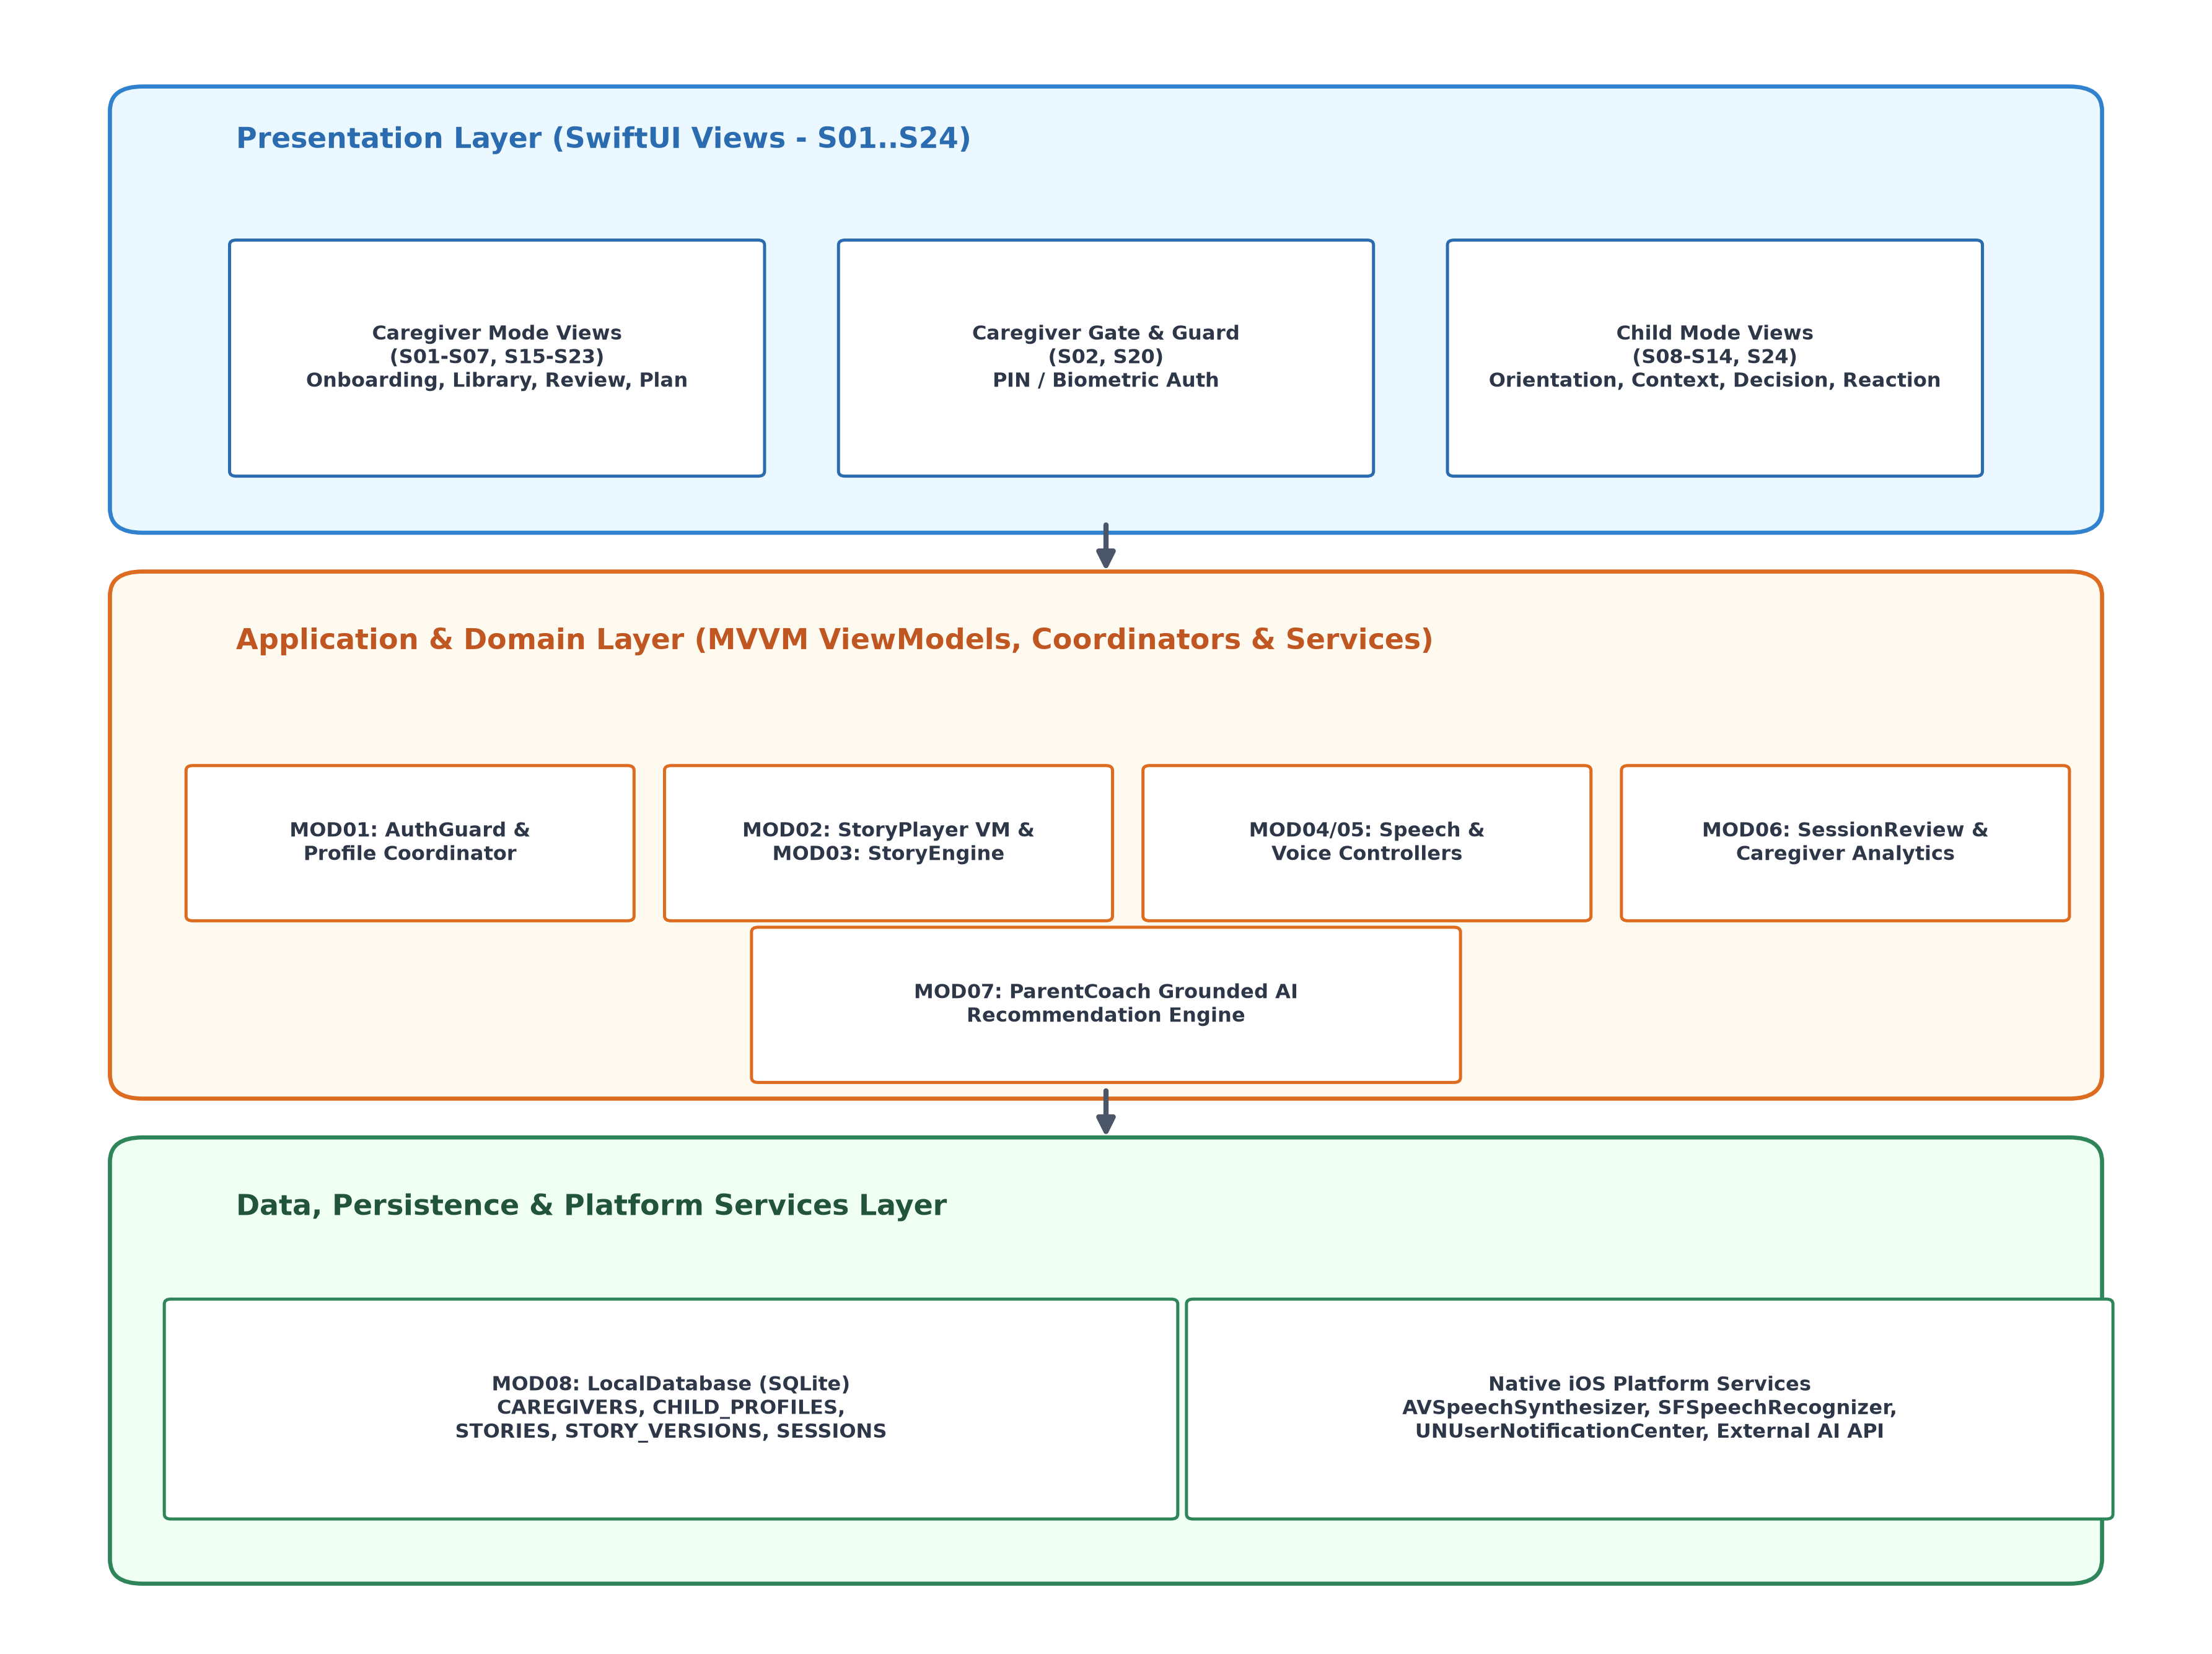
\includegraphics[width=0.95\textwidth]{figures/system_architecture.png}
\caption{Three-Layer Offline-First and Mode-Separated System Architecture}
\label{fig:system_architecture}
\end{figure}



\subsection{Technology Choices and Cross-Device Data Strategy}


\noindent\begin{xltabular}{\textwidth}{|p{3.2cm}|p{4.0cm}|X|}
\hline
\textbf{Architectural Layer} & \textbf{Selected Technology} & \textbf{Rationale and Alignment with Bear Buddy Requirements} \\ \hline
\endhead
\textbf{Mobile Platform \& UI Framework} & \textbf{iOS / iPadOS 17.0+} with \textbf{SwiftUI} & Declarative reactive UI with native support for Dynamic Type ($200\%$ font scaling), VoiceOver, Reduce Motion, and precise hit-target sizing (\texttt{NFR01}–\texttt{NFR07}). \\ \hline
\textbf{Frontend Architecture} & \textbf{MVVM (Model – View – ViewModel)} & Decouples the interactive story state machine (\texttt{Understand} $\rightarrow$ \texttt{Predict} $\rightarrow$ \texttt{Choose} $\rightarrow$ \texttt{Observe} $\rightarrow$ \texttt{Why} $\rightarrow$ \texttt{Repeat}) from SwiftUI views, enabling deterministic unit testing of story branches and system states (\texttt{S23}). \\ \hline
\textbf{Local Relational Database} & \textbf{SQLite3} (\texttt{LocalDatabase}) & Lightweight, ACID-compliant relational storage with foreign-key enforcement; supports structured multi-version story storage (\texttt{story\_version}), role-based access links, and granular interaction logs without requiring a mandatory backend server. \\ \hline
\textbf{Cross-Device Data Exchange Strategy} & \textbf{Local SQLite + Controlled Encrypted Sync/Export Package} & Addresses the architectural note in Section 1.4.2: SQLite serves as the primary local source of truth; when a parent (\texttt{PERS02}) links a profile with a support teacher (\texttt{PERS03}), only the authorized child profile and versioned session logs are synchronized/exported within the explicitly granted scope. \\ \hline
\textbf{Audio Narration \& Speech Recognition} & \textbf{AVFoundation (\texttt{AVSpeechSynthesizer})} \& \textbf{Speech (\texttt{SFSpeechRecognizer})} & Enables single-stream audio queue management to prevent overlapping narration (\texttt{DD23}), adjustable Vietnamese speech rates, and on-device keyword recognition for Scenario E. \\ \hline
\textbf{Local Activity Reminders} & \textbf{UserNotifications (\texttt{UNUserNotificationCenter})} & Schedules caregiver activity reminders locally on the device without relying on third-party push notification servers. \\ \hline
\end{xltabular}



\section{Module Design and Complete Traceability Matrix}



\subsection{Module Responsibilities}


The system is decomposed into 8 cohesive modules (\texttt{MOD01}–\texttt{MOD08}):

\begin{itemize}
  \item \textbf{\texttt{MOD01} — Account, Profile \& Role Guard Module (\texttt{ProfileModels}, \texttt{CaregiverGate})}: Manages caregiver authentication, child profile CRUD, role-based access control between Parent (\texttt{PERS02}) and Support Teacher (\texttt{PERS03}), and privacy consent audit logging (\texttt{consent\_audit\_logs}).
  \item \textbf{\texttt{MOD02} — Versioned Story Library Module (\texttt{StoryRepository}, \texttt{StoryModels})}: Manages story retrieval across the 4 situational categories (\texttt{CAT01}–\texttt{CAT04}), keyword/filter queries, transparent popularity metrics, and immutable \texttt{story\_version} resolution.
  \item \textbf{\texttt{MOD03} — Interactive Story Engine Module (\texttt{StoryPlayerViewModel})}: The core state machine governing \texttt{Child Mode} sessions, handling \texttt{Choice Card} and \texttt{Tap-to-Order} inputs, routing \texttt{Action} $\rightarrow$ \texttt{Reaction} $\rightarrow$ \texttt{Why} branches, and executing \texttt{Replay}, \texttt{Retry}, \texttt{Pause}, and \texttt{Need Help}.
  \item \textbf{\texttt{MOD04} — Accessibility \& Audio Narration Module (\texttt{SpeechController}, \texttt{AppColors})}: Applies per-profile font scaling, contrast tokens, and motion settings, and enforces single-stream narration playback so multiple taps never overlap audio.
  \item \textbf{\texttt{MOD05} — Scenario E Voice \& Touch Fallback Module (\texttt{VoiceInteractionController})}: Manages bounded short-phrase practice on \texttt{S24}, checks microphone permissions, performs keyword matching, and guarantees immediate touch-card fallback on error or refusal.
  \item \textbf{\texttt{MOD06} — Session Logger, Review \& Plan Module (\texttt{ParentViews}, \texttt{ReminderService})}: Records chronological child interaction events pinned to \texttt{story\_version}, renders descriptive \texttt{Session Review} screens (\texttt{S15}, \texttt{S16}), and manages \texttt{Learning Plans} and reminders (\texttt{S17}, \texttt{S19}).
  \item \textbf{\texttt{MOD07} — Explainable Parent AI Coach Module (\texttt{ParentCoachService})}: Combines local rule-based filtering with grounded AI queries to recommend library stories accompanied by human-readable match reasons (\texttt{S18}).
  \item \textbf{\texttt{MOD08} — Local Persistence \& System State Module (\texttt{LocalDatabase}, \texttt{AppStore})}: Provides transactional SQLite3 data access, manages the offline feedback queue (\texttt{S22}), and coordinates system/error states (\texttt{S23}).
\end{itemize}



\subsection{Complete Traceability Matrix}


Completing the requirement established in Section 5.7.3, the table below provides end-to-end traceability linking \textbf{User Needs (\texttt{UN}) $\rightarrow$ Requirements (\texttt{FR}/\texttt{NFR}) $\rightarrow$ Use Cases (\texttt{UC}) $\rightarrow$ UX Decisions (\texttt{DD}) $\rightarrow$ Screens (\texttt{S}) $\rightarrow$ Architecture Modules (\texttt{MOD})}:

\begin{footnotesize}
\noindent\begin{xltabular}{\textwidth}{|p{1.5cm}|p{2.2cm}|X|p{2.0cm}|p{2.0cm}|p{1.8cm}|}
\hline
\textbf{User Need (\texttt{UN})} & \textbf{Requirements (\texttt{FR} / \texttt{NFR})} & \textbf{Use Cases (\texttt{UC})} & \textbf{UX Decisions (\texttt{DD})} & \textbf{Screens (\texttt{S01}–\texttt{S24})} & \textbf{Architecture Modules (\texttt{MOD})} \\ \hline
\endhead
\textbf{UN01} (Understand context prior to choice) & \texttt{FR09}, \texttt{FR10} & \texttt{UC04}, \texttt{UC06} & \texttt{DD13}, \texttt{DD14} & \texttt{S07}, \texttt{S09} & \texttt{MOD02}, \texttt{MOD03} \\ \hline
\textbf{UN02} (Participate without independent reading) & \texttt{FR05}, \texttt{FR10}, \texttt{FR11}, \texttt{NFR01}, \texttt{NFR06} & \texttt{UC03}, \texttt{UC06} & \texttt{DD7}–\texttt{DD12}, \texttt{DD20} & \texttt{S04}, \texttt{S08}, \texttt{S09} & \texttt{MOD03}, \texttt{MOD04} \\ \hline
\textbf{UN03} (Clear orientation \& predictability) & \texttt{FR05}, \texttt{FR10}, \texttt{FR16}, \texttt{NFR09}, \texttt{NFR10} & \texttt{UC06}, \texttt{UC08} & \texttt{DD2}–\texttt{DD6} & \texttt{S08}–\texttt{S12}, \texttt{S14} & \texttt{MOD03} \\ \hline
\textbf{UN04} (Forgiving tap input \& non-mandatory voice) & \texttt{FR12}, \texttt{FR18}, \texttt{NFR03}, \texttt{NFR04}, \texttt{NFR06} & \texttt{UC07}, \texttt{UC10} & \texttt{DD26}–\texttt{DD30}, \texttt{DD36} & \texttt{S10}, \texttt{S24} & \texttt{MOD03}, \texttt{MOD05} \\ \hline
\textbf{UN05} (Understand Why, Replay \& Retry) & \texttt{FR13}, \texttt{FR14} & \texttt{UC08} & \texttt{DD15}–\texttt{DD19} & \texttt{S11}, \texttt{S12} & \texttt{MOD03}, \texttt{MOD06} \\ \hline
\textbf{UN06} (Sensory control \& self-paced learning) & \texttt{FR03}, \texttt{FR11}, \texttt{FR15}, \texttt{FR16}, \texttt{NFR05}, \texttt{NFR08} & \texttt{UC03}, \texttt{UC06}, \texttt{UC09} & \texttt{DD21}–\texttt{DD23}, \texttt{DD34}, \texttt{DD37} & \texttt{S04}, \texttt{S09}–\texttt{S14} & \texttt{MOD03}, \texttt{MOD04} \\ \hline
\textbf{UN07} (Caregiver library search \& story preview) & \texttt{FR01}, \texttt{FR06}–\texttt{FR09}, \texttt{FR21} & \texttt{UC01}, \texttt{UC04}, \texttt{UC12} & \texttt{DD31}, \texttt{DD32} & \texttt{S01}, \texttt{S05}–\texttt{S07}, \texttt{S17} & \texttt{MOD01}, \texttt{MOD02}, \texttt{MOD06} \\ \hline
\textbf{UN08} (Version-pinned \& profile-scoped review) & \texttt{FR02}–\texttt{FR04}, \texttt{FR19}–\texttt{FR22}, \texttt{NFR16} & \texttt{UC02}, \texttt{UC11}, \texttt{UC12} & \texttt{DD31}–\texttt{DD33}, \texttt{DD38} & \texttt{S02}, \texttt{S03}, \texttt{S15}, \texttt{S16} & \texttt{MOD01}, \texttt{MOD06}, \texttt{MOD08} \\ \hline
\textbf{UN09} (Explainable \& reviewable AI suggestions) & \texttt{FR17}, \texttt{FR18}, \texttt{NFR15} & \texttt{UC05}, \texttt{UC10} & \texttt{DD36}, \texttt{DD39} & \texttt{S18}, \texttt{S24} & \texttt{MOD05}, \texttt{MOD07} \\ \hline
\textbf{UN10} (Child agency to Pause or Ask for Help) & \texttt{FR15}, \texttt{NFR08} & \texttt{UC09} & \texttt{DD37} & \texttt{S08}–\texttt{S13} & \texttt{MOD03}, \texttt{MOD06} \\ \hline
\textbf{UN11} (Child data minimization \& access control) & \texttt{FR01}–\texttt{FR04}, \texttt{FR23}, \texttt{NFR14}, \texttt{NFR15} & \texttt{UC01}, \texttt{UC02}, \texttt{UC13} & \texttt{DD33}, \texttt{DD34}, \texttt{P11} & \texttt{S01}–\texttt{S03}, \texttt{S20} & \texttt{MOD01}, \texttt{MOD08} \\ \hline
\textbf{UN12} (Resilient error handling, Offline \& Support) & \texttt{FR18}, \texttt{FR22}, \texttt{FR24}, \texttt{FR25}, \texttt{NFR12}, \texttt{NFR13} & \texttt{UC04}, \texttt{UC05}, \texttt{UC10}, \texttt{UC14} & \texttt{DD24}, \texttt{DD40} & \texttt{S21}–\texttt{S24} & \texttt{MOD05}, \texttt{MOD07}, \texttt{MOD08} \\ \hline
\end{xltabular}
\end{footnotesize}



\section{SQLite Database Design}


The local SQLite database (\texttt{MOD08 - LocalDatabase}) is normalized to guarantee: (1) strict separation between caregiver accounts, child profiles, and revocable teacher access links; (2) immutable multi-version story storage (\texttt{story\_versions}) so historical session reviews remain accurate even after content updates; and (3) descriptive, non-punitive interaction logging.


\subsection{Entity-Relationship Diagram (ERD)}



\begin{figure}[htbp]
\centering
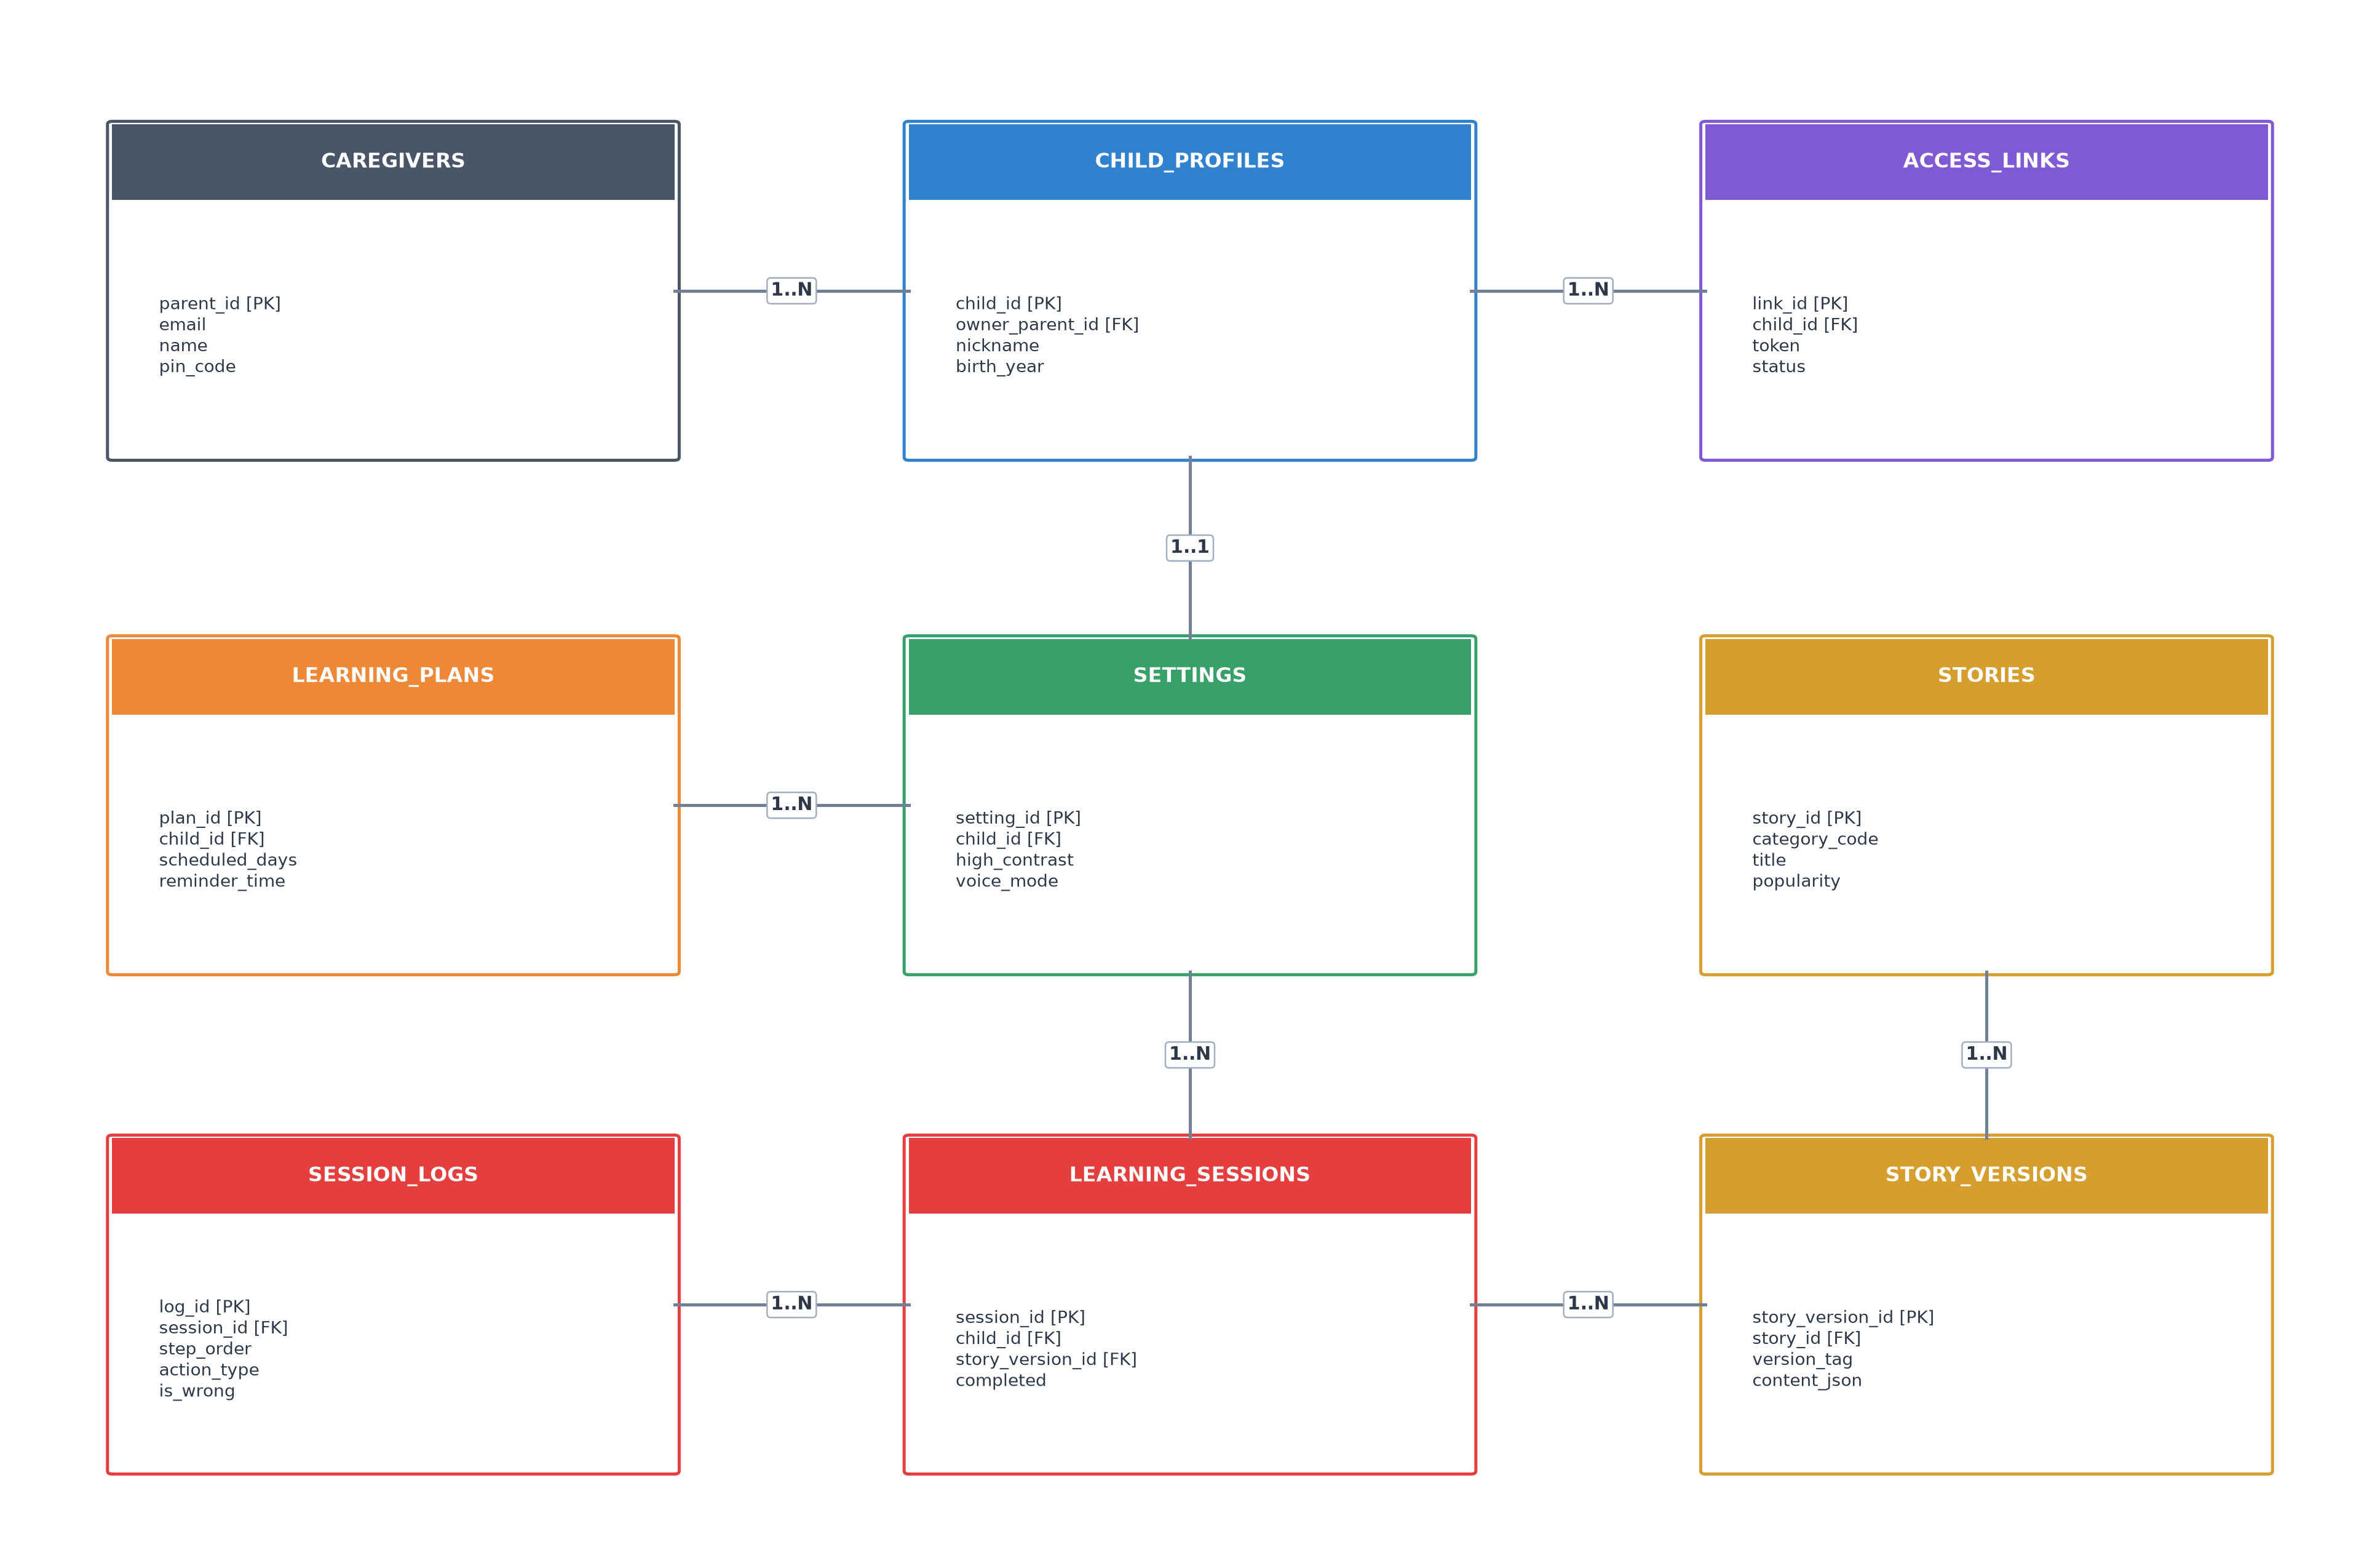
\includegraphics[width=0.95\textwidth]{figures/sqlite_erd.png}
\caption{SQLite Entity-Relationship Diagram (ERD)}
\label{fig:sqlite_erd}
\end{figure}



\subsection{Key Schema Design Decisions}


\begin{enumerate}
  \item \textbf{Separation of \texttt{STORIES} and \texttt{STORY\_VERSIONS} (\texttt{FR09}, \texttt{FR20})}:
\end{enumerate}
\begin{itemize}
  \item The \texttt{STORIES} table holds the canonical story identifier and category, whereas all scene steps, choice cards, and \texttt{why\_explanation\_text} records belong to an immutable \texttt{STORY\_VERSIONS} record.
  \item \texttt{LEARNING\_SESSIONS} references both \texttt{story\_id} and \texttt{story\_version\_id}. When a caregiver opens \texttt{Session Review} (\texttt{S16}) for a historical session, the query joins on \texttt{story\_version\_id} to render the exact wording and explanation the child saw during that session, even if the story was subsequently updated.
\end{itemize}
\begin{enumerate}
  \item \textbf{Non-Punitive Event Logging in \texttt{SESSION\_INTERACTIONS} (\texttt{DD17}, \texttt{DD18}, \texttt{DD38})}:
\end{enumerate}
\begin{itemize}
  \item \texttt{SESSION\_INTERACTIONS} intentionally omits \texttt{score} or \texttt{is\_wrong} columns. Instead, it records a chronological stream of behavioral events (\texttt{CHOOSE\_TAP}, \texttt{CHOOSE\_VOICE}, \texttt{REPLAY}, \texttt{RETRY}, \texttt{PAUSE}, \texttt{HELP}) alongside \texttt{attempt\_number}, allowing caregivers to understand how the child explored the scenario without reducing the session to a diagnostic grade.
\end{itemize}
\begin{enumerate}
  \item \textbf{Scoped Teacher Authorization via \texttt{PROFILE\_ACCESS\_LINKS} (\texttt{FR04})}:
\end{enumerate}
\begin{itemize}
  \item Every query fetching child profiles or session histories for a user with \texttt{role\_type = 'TEACHER'} enforces an \texttt{INNER JOIN} against \texttt{PROFILE\_ACCESS\_LINKS} filtered by \texttt{link\_status = 'ACTIVE'}.
\end{itemize}



\section{Sequence Diagrams and State Diagram}



\subsection{Sequence Diagram 1: Story Learning Flow and Version-Pinned Caregiver Review}


The sequence diagram below illustrates the end-to-end flow from caregiver story preview and \texttt{Child Mode} launch, through the child's \texttt{Understand} $\rightarrow$ \texttt{Predict} $\rightarrow$ \texttt{Choose} $\rightarrow$ \texttt{Observe} $\rightarrow$ \texttt{Understand Why} $\rightarrow$ \texttt{Repeat} loop, to the version-pinned caregiver review:


\begin{figure}[htbp]
\centering
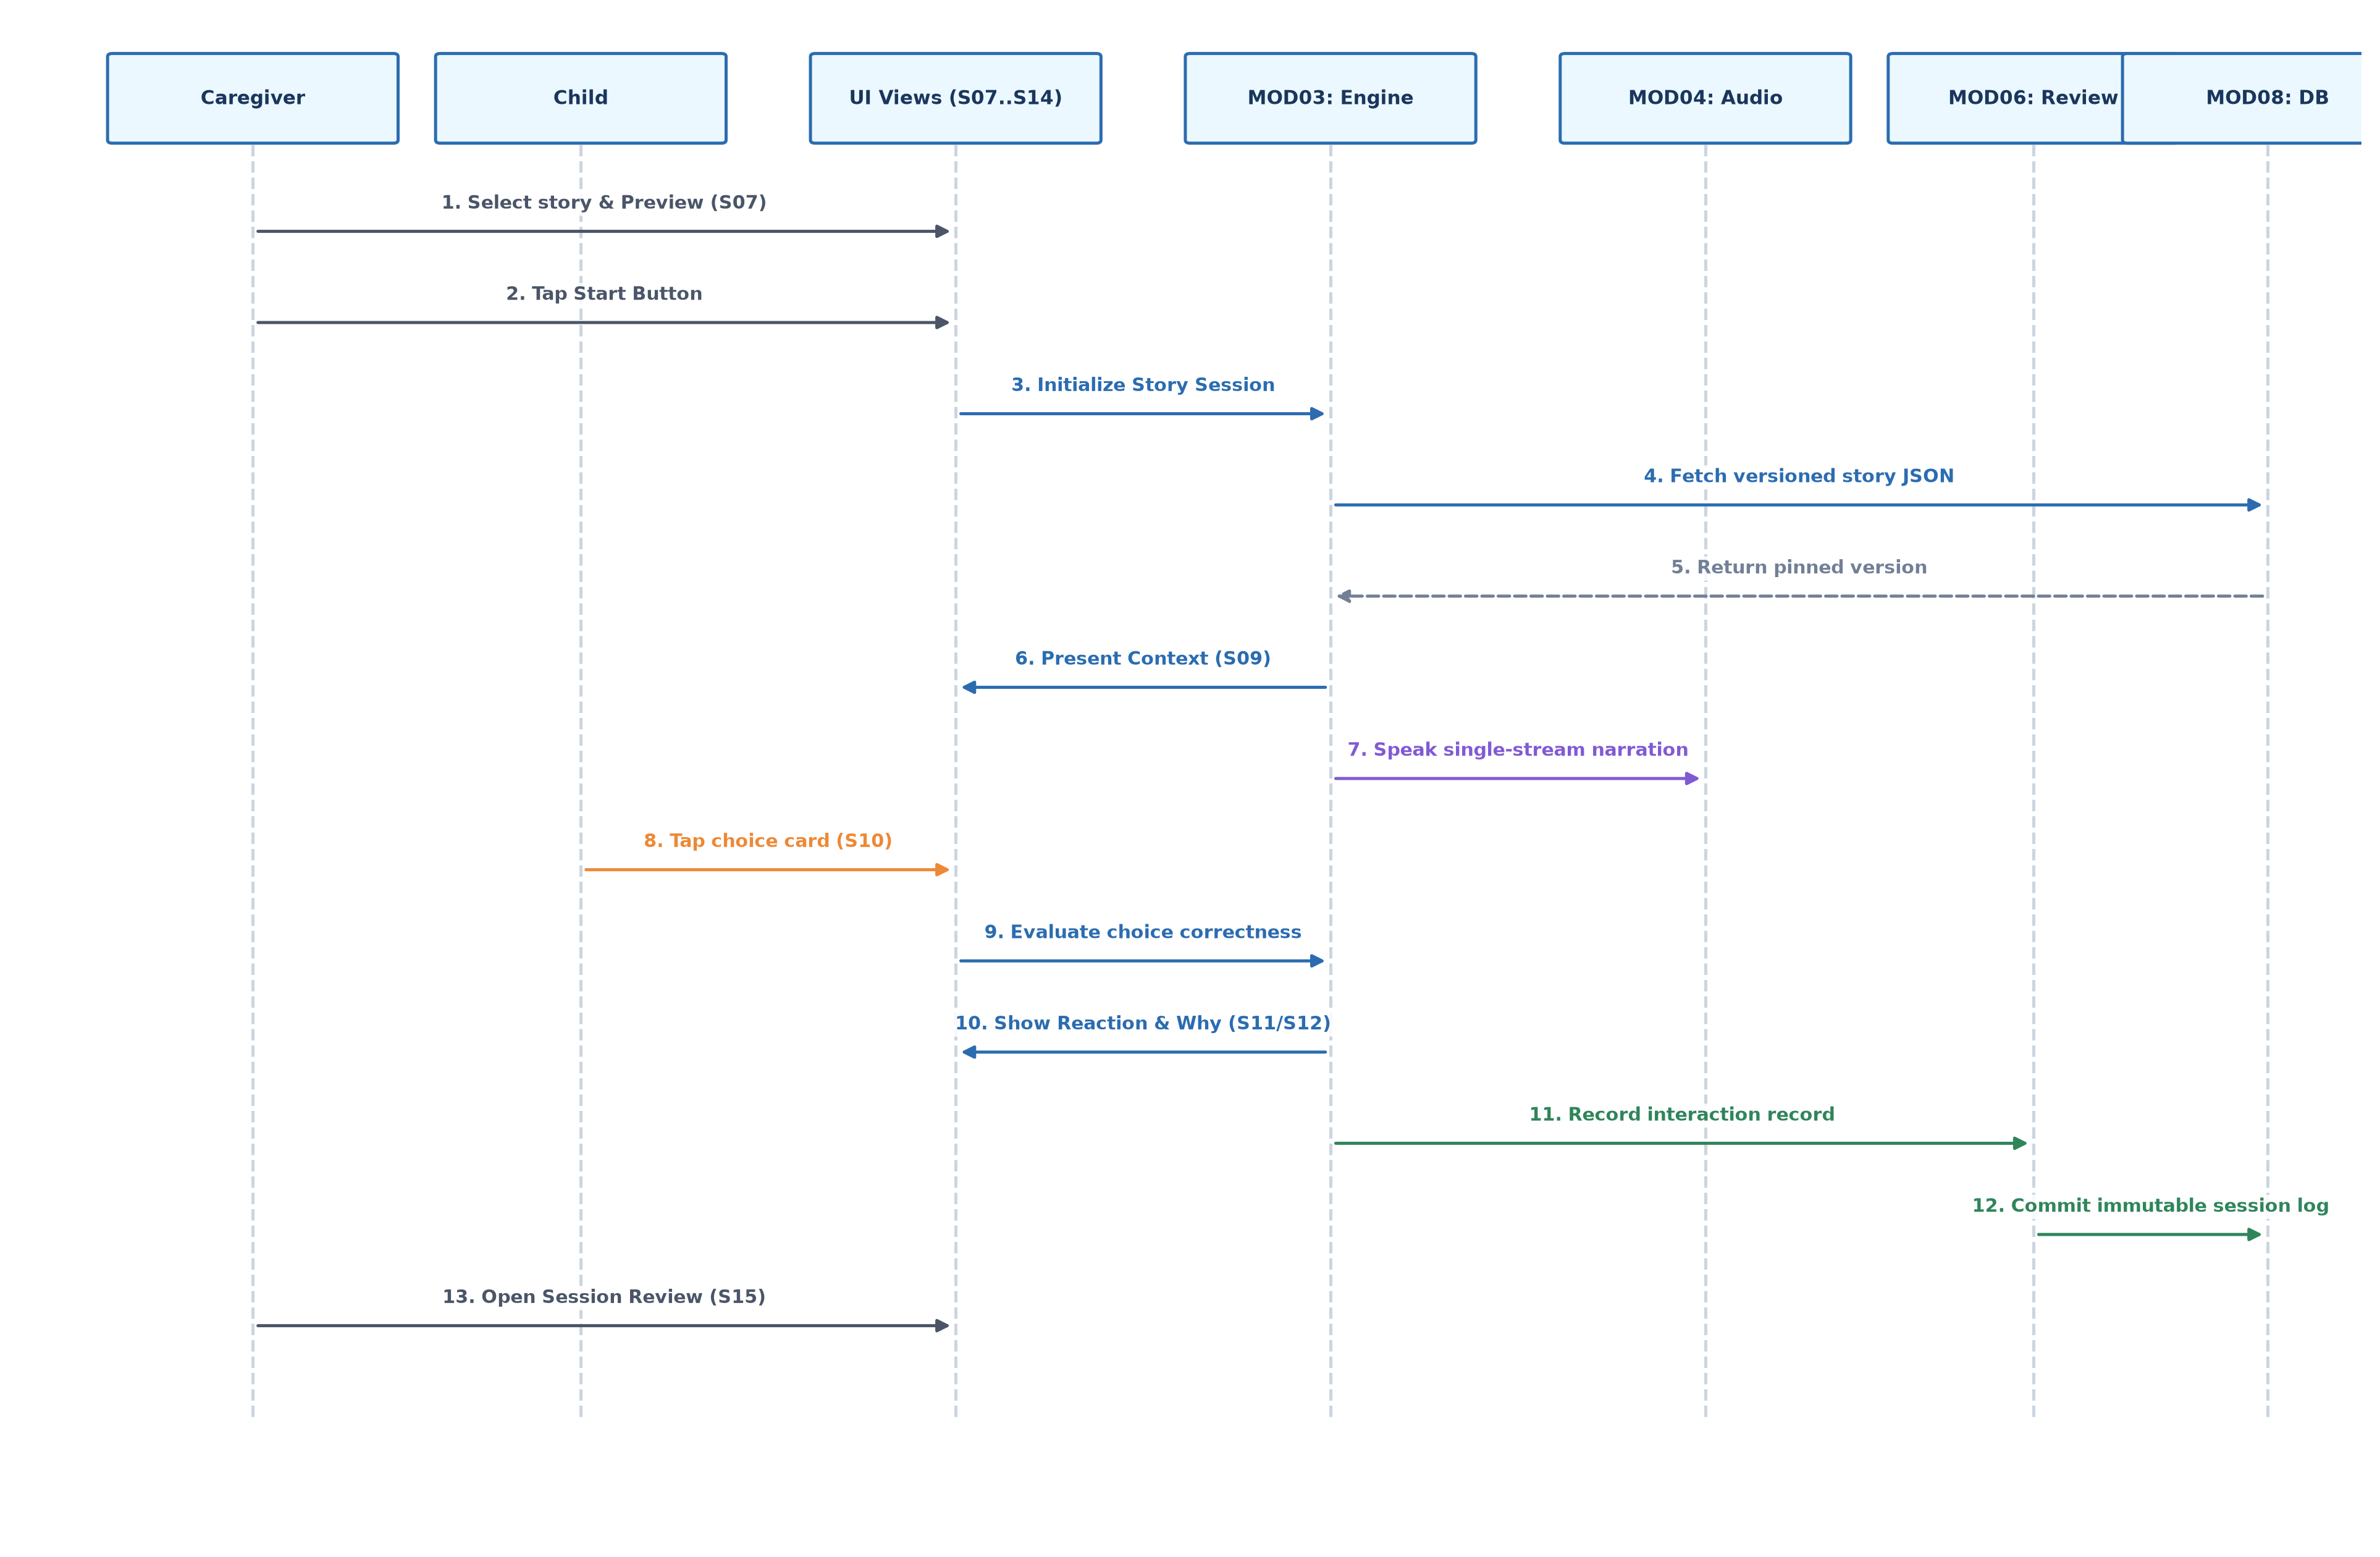
\includegraphics[width=0.95\textwidth]{figures/sequence_story_learning.png}
\caption{Sequence Diagram: Story Learning Flow and Version-Pinned Review}
\label{fig:sequence_story_learning}
\end{figure}



\subsection{Sequence Diagram 2: Scenario E Voice Interaction and Touch Fallback Flow}


The second sequence diagram models the bounded voice interaction in Scenario E (\texttt{S24}), illustrating how the child can always complete the step via touch cards if microphone access is denied or speech is not recognized:


\begin{figure}[htbp]
\centering
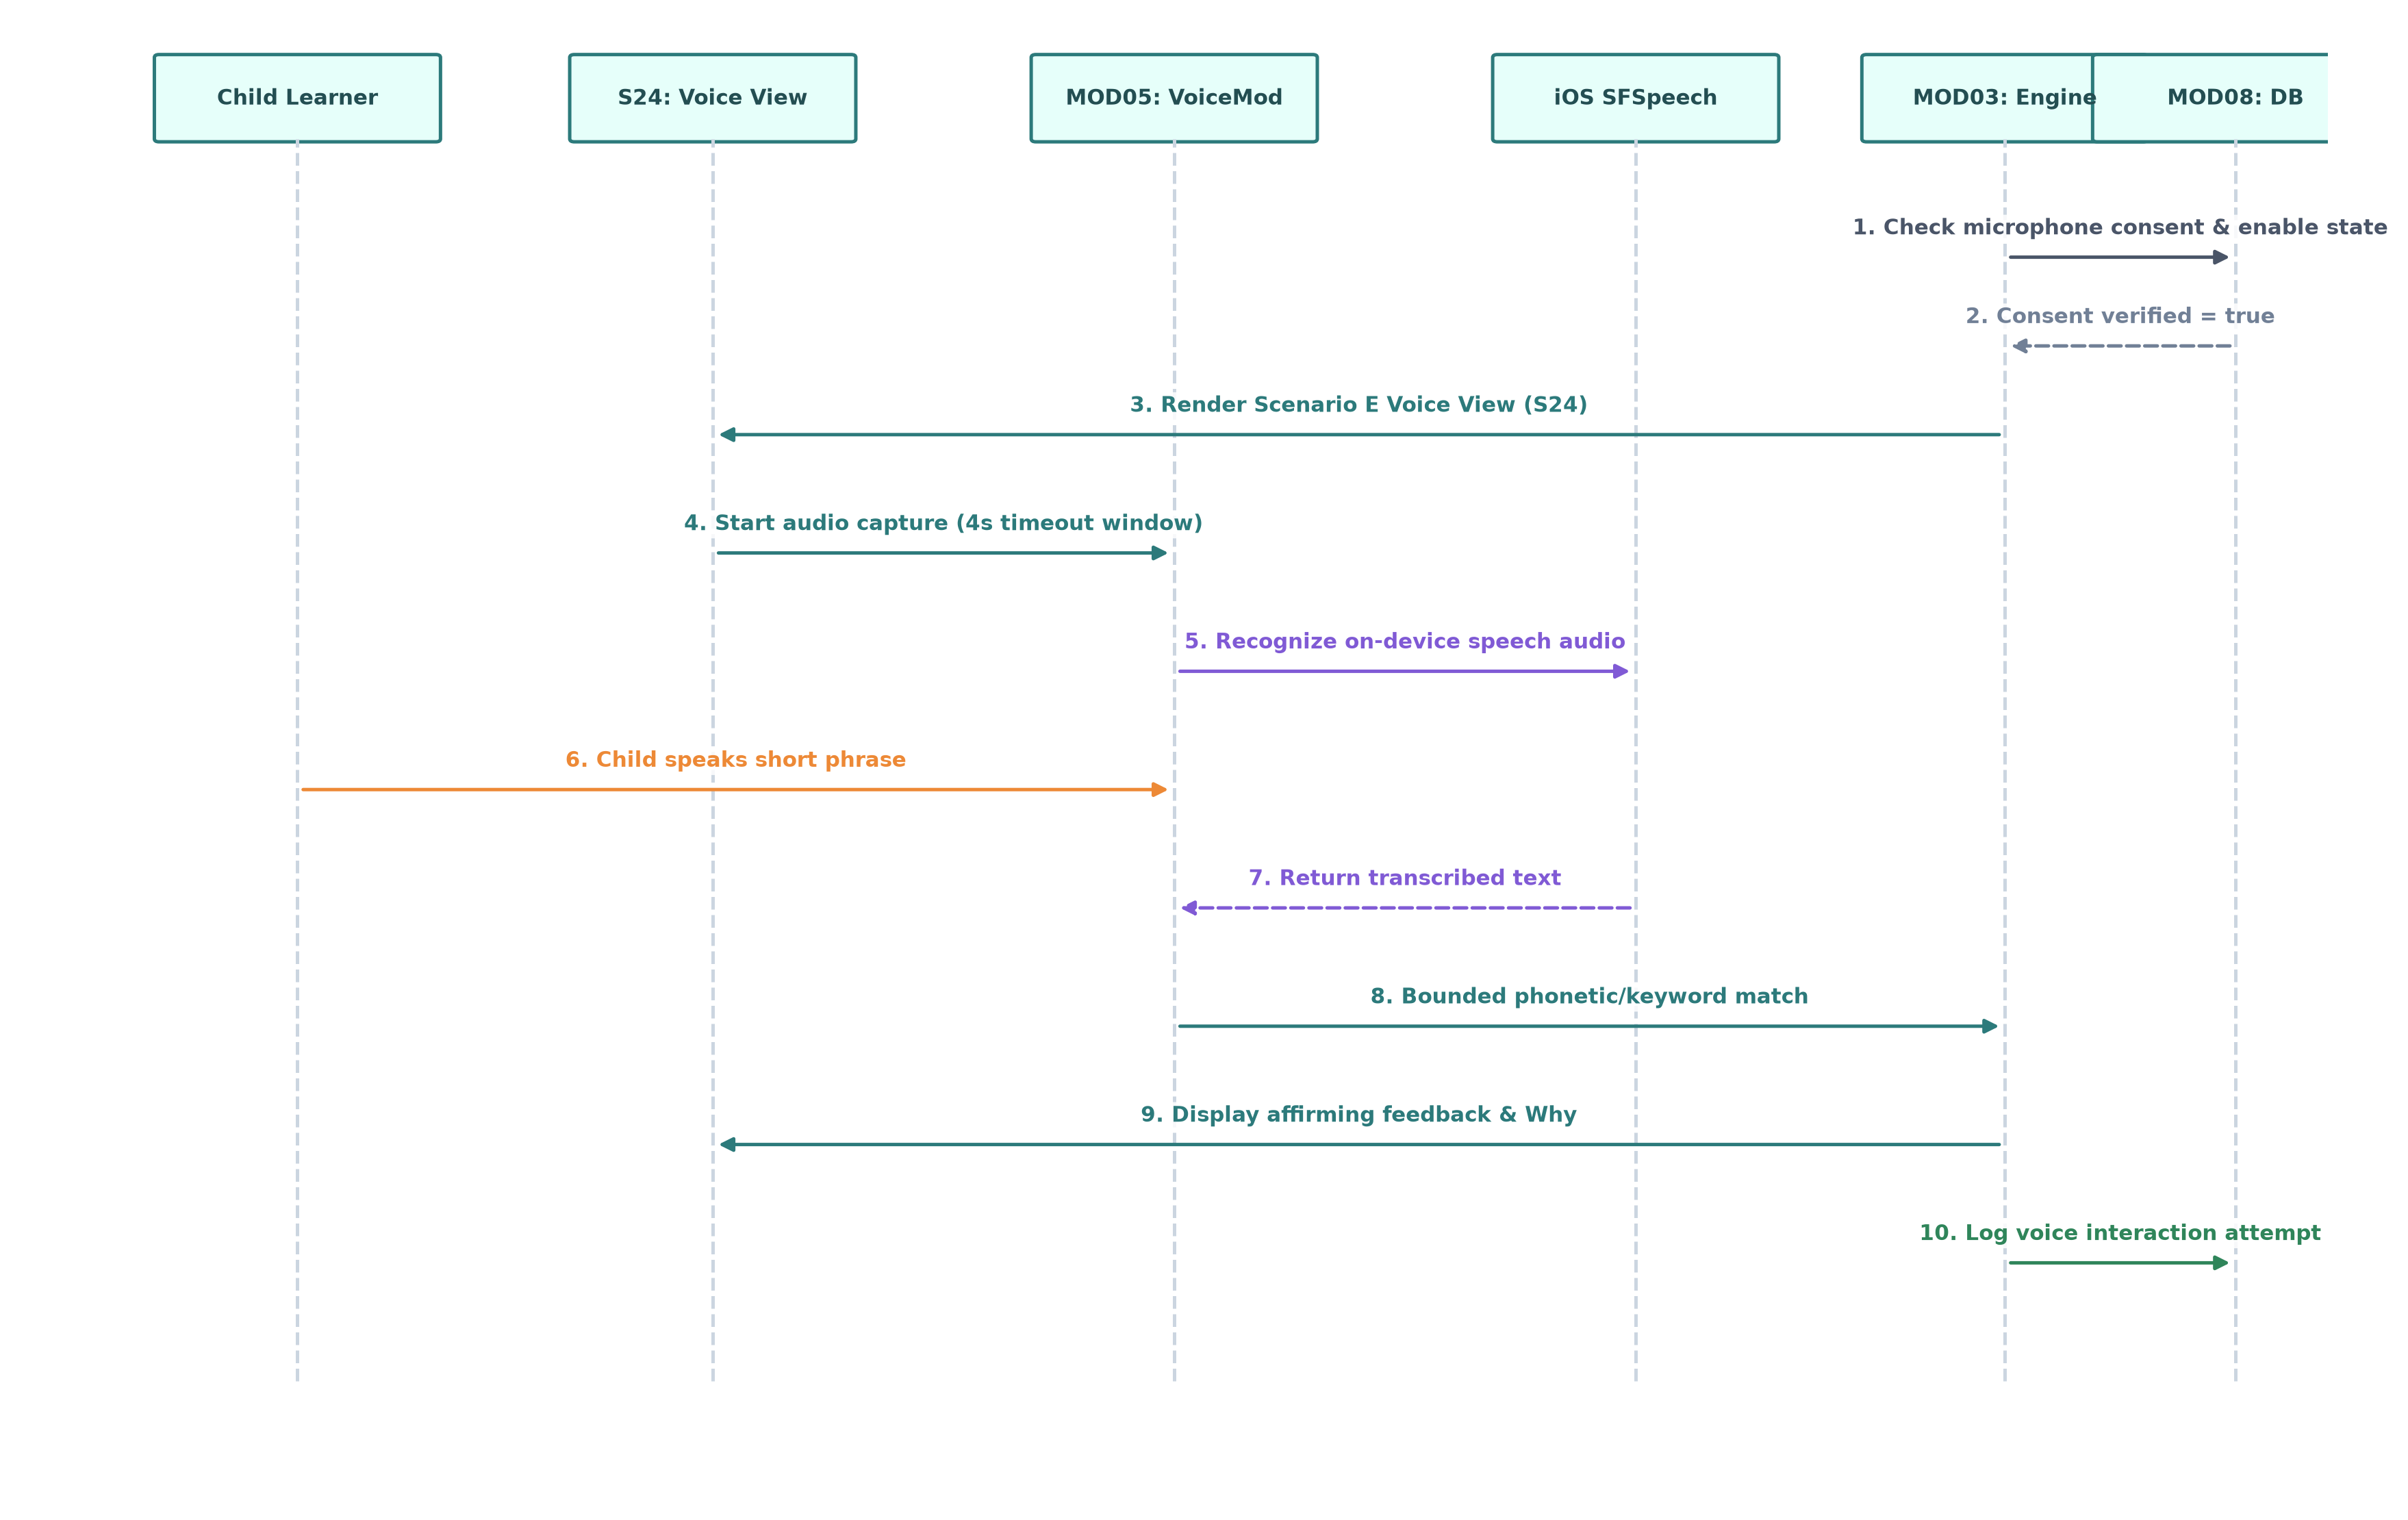
\includegraphics[width=0.95\textwidth]{figures/sequence_voice_interaction.png}
\caption{Sequence Diagram: Scenario E Voice Interaction and Touch Fallback Flow}
\label{fig:sequence_voice_interaction}
\end{figure}



\subsection{State Diagram: Story Player State Machine}


The state machine diagram below specifies the lifecycle of an interactive story session, ensuring that pausing, requesting help, or encountering an error preserves the child's context (\texttt{DD37}, \texttt{DD40}):


\begin{figure}[htbp]
\centering
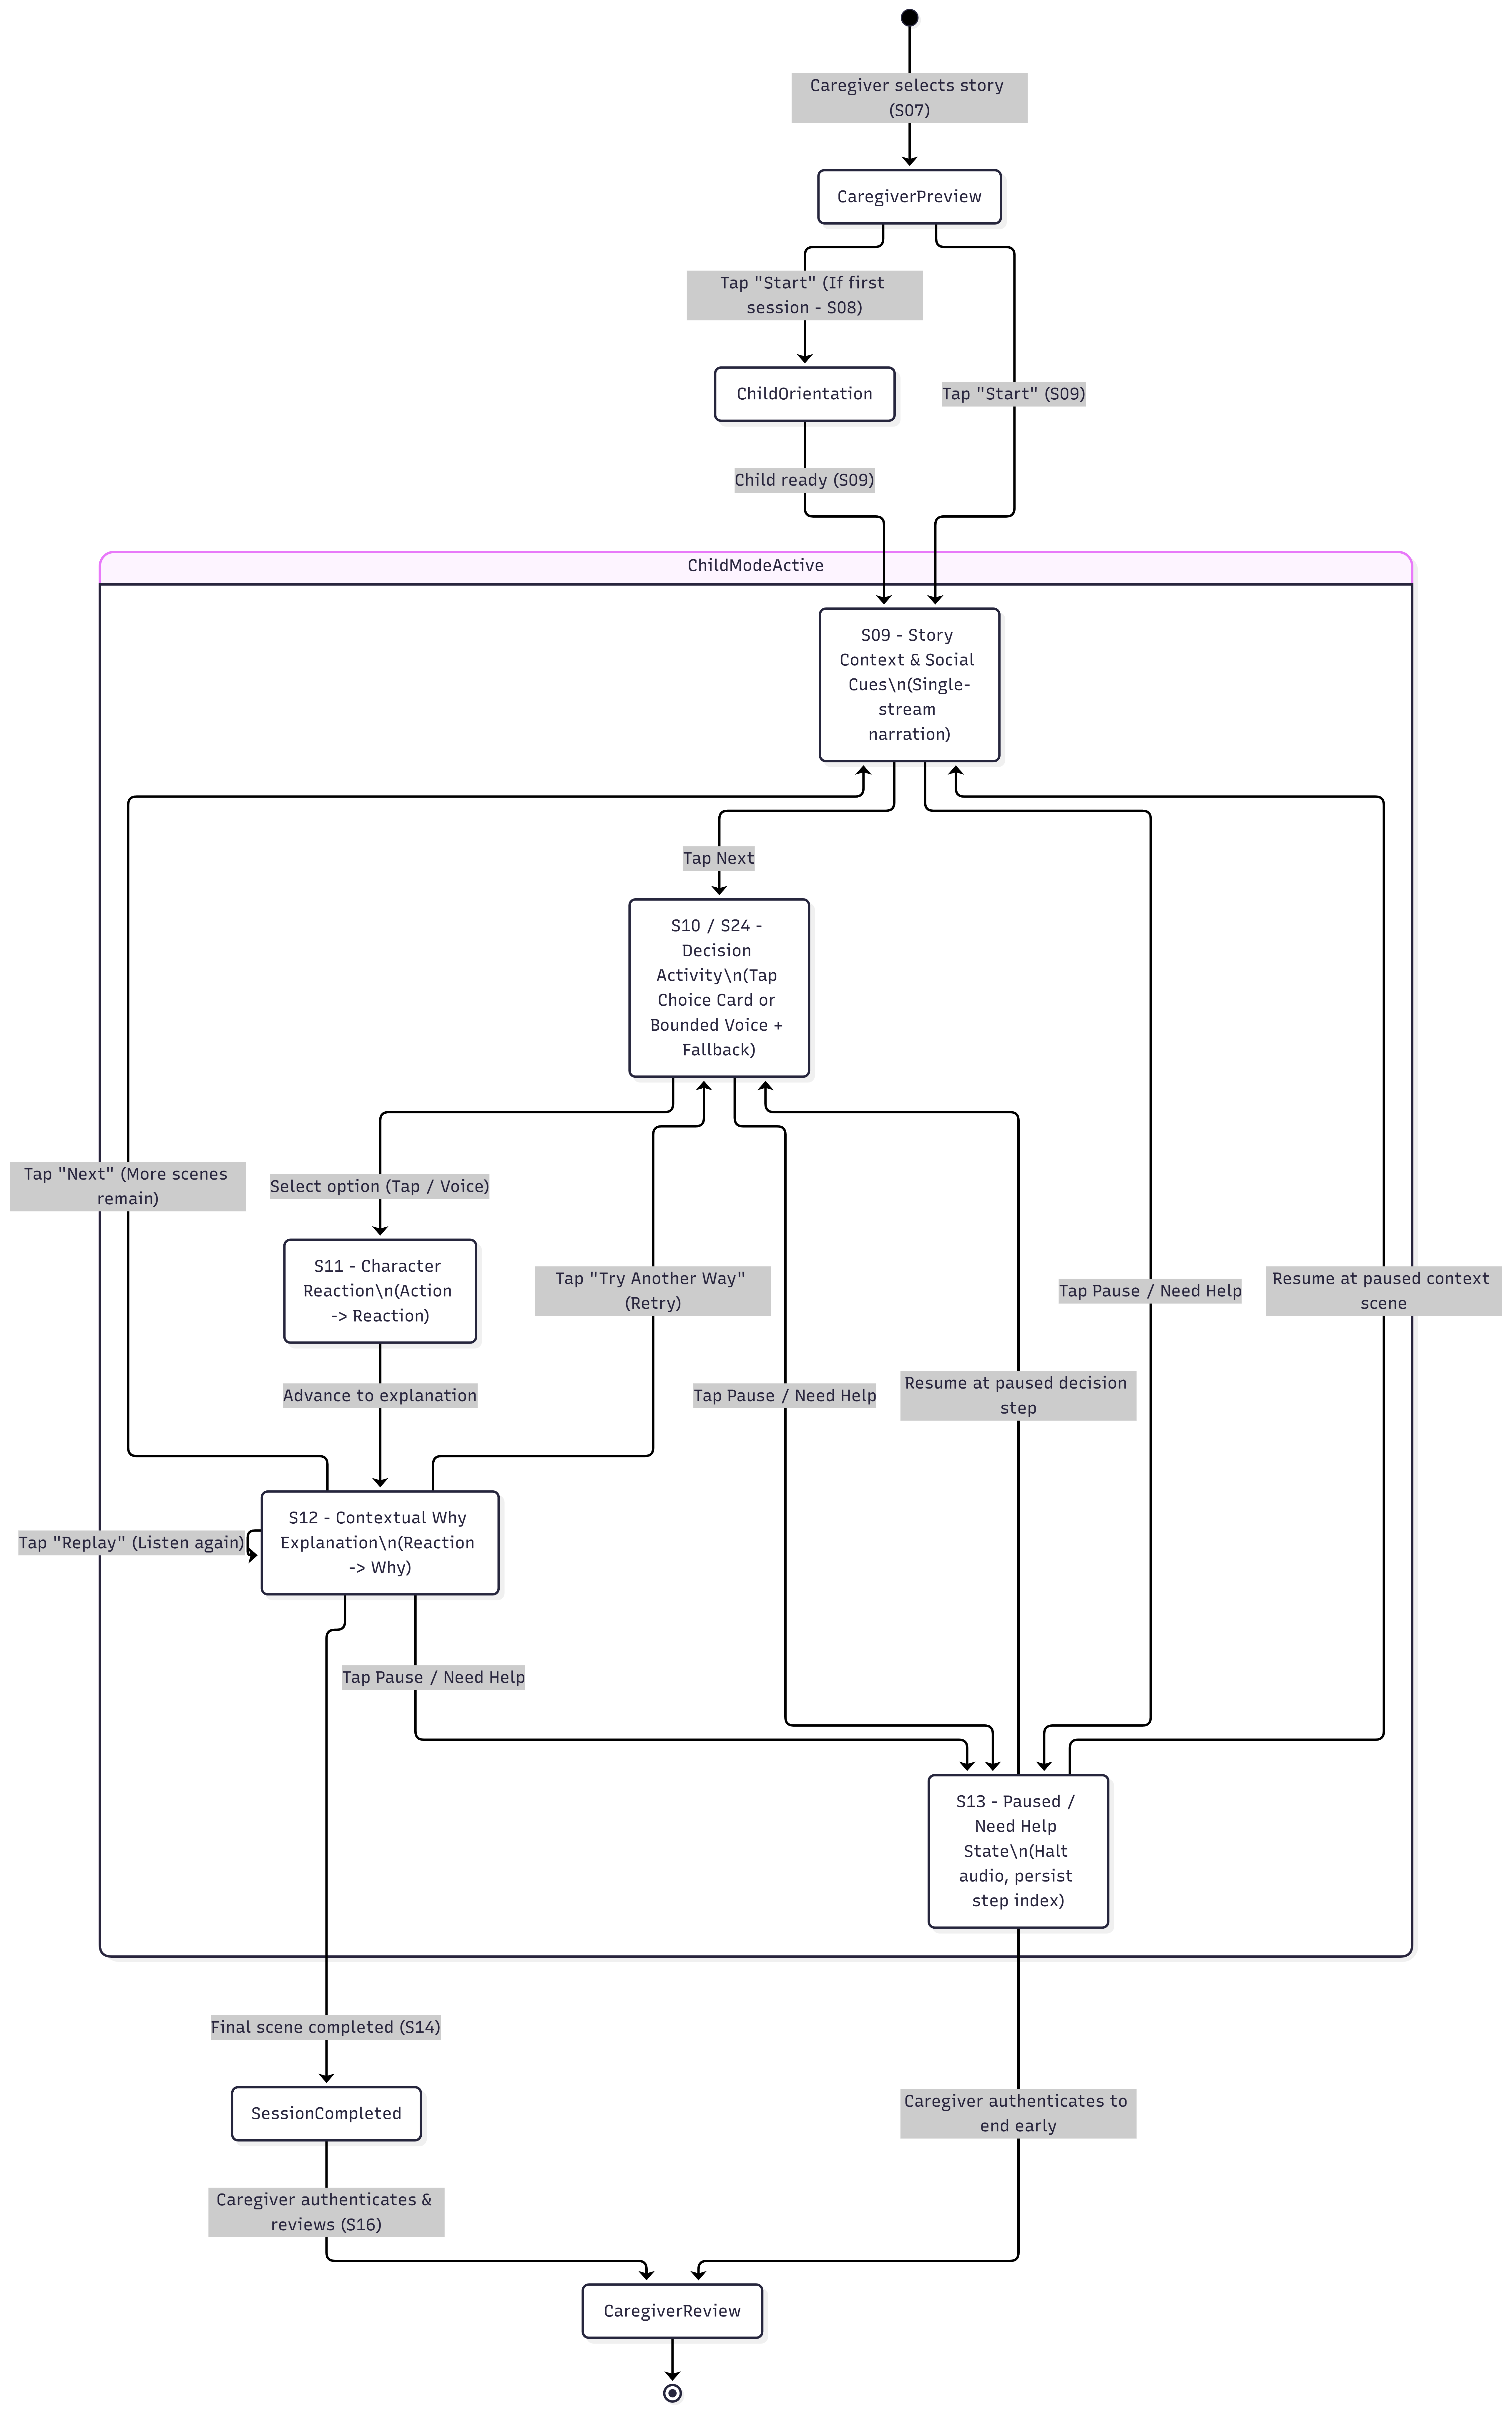
\includegraphics[width=0.95\textwidth]{figures/state_machine.png}
\caption{State Diagram: Story Player State Machine}
\label{fig:state_machine}
\end{figure}



\section{AI and Voice Interaction Design}



\subsection{Explainable Hybrid Grounded AI Recommendation for Parents (\texttt{MOD07})}


To satisfy \texttt{UN09}, \texttt{FR17}, and \texttt{DD39}, the Parent AI Suggestion feature on screen \texttt{S18} is designed around a \textbf{Hybrid Grounded Recommendation Architecture}:

\begin{enumerate}
  \item \textbf{Strict Library Grounding}: The AI module never fabricates unreviewed stories. Its input is strictly bounded to: (a) the situational goal selected or entered by the parent, (b) anonymizable recent story IDs (only if opted in on \texttt{S20}), and (c) the catalog of verified \texttt{STORIES} and \texttt{STORY\_VERSIONS} in the library.
  \item \textbf{Explainable Output Schema}: Every recommendation returned to \texttt{S18} must contain three structured fields:
\end{enumerate}
\begin{itemize}
  \item \texttt{recommended\_story\_id}: A valid story identifier existing in the local library.
  \item \texttt{match\_reason\_text}: A clear, human-readable explanation of why this story matches the parent's stated goal (e.g., \textit{"Recommended because it introduces the stethoscope sensation and practices signaling Mom when feeling nervous at the clinic"}).
  \item \texttt{alternative\_category\_code}: A related category tag allowing the parent to browse other options freely.
\end{itemize}
\begin{enumerate}
  \item \textbf{Deterministic Local Rule-Based Fallback}: When the device is offline, AI history consent is disabled, or the API exceeds the \textbf{$5\text{-second}$} timeout (\texttt{AI Timeout}), \texttt{ParentCoachService} automatically switches to local keyword and category-tag matching against SQLite so the parent always receives immediate, explainable suggestions.
\end{enumerate}



\subsection{Bounded On-Device Voice Interaction for Scenario E (\texttt{MOD05})}


\begin{itemize}
  \item \textbf{No Open-Ended Generative Voice Chat (\texttt{DD36})}: To eliminate unpredictable AI responses and expressive language pressure, Scenario E (\texttt{S24}) uses native speech recognition (\texttt{SFSpeechRecognizer} with \texttt{requiresOnDeviceRecognition} enabled where supported) strictly to match keywords against pre-authored target phrases.
  \item \textbf{Lenient Keyword Matching \& Zero Pronunciation Grading}: Detection of any core functional keyword from the model phrase (e.g., matching \textit{"play"} or \textit{"join"} for \textit{"Can I play too?"}) is accepted as a valid communicative attempt.
  \item \textbf{First-Class Parallel Touch Alternative}: Illustrated choice cards remain visible and active alongside the microphone button on \texttt{S24} at all times.
\end{itemize}



\section{Privacy and Security Design}


Bear Buddy's privacy and security architecture operationalizes \textbf{Privacy and Agency by Design (\texttt{P11})} and aligns with UNICEF's Guidance on AI and Children:

\noindent\begin{xltabular}{\textwidth}{|p{4.0cm}|X|}
\hline
\textbf{Privacy \& Security Dimension} & \textbf{Technical Implementation in Bear Buddy} \\ \hline
\endhead
\textbf{1. Data Minimization \& Ephemeral Voice Processing (\texttt{DD33}, \texttt{NFR14})} & $\bullet$ Child profiles store only a display \texttt{nickname} and functional support settings; full legal names, exact birthdates, home addresses, and clinical diagnoses are never collected. \newline $\bullet$ Microphone audio in Scenario E (\texttt{S24}) is processed exclusively in volatile RAM buffers for keyword matching and deallocated immediately after the step completes; no audio files are ever written to disk or transmitted externally. \\ \hline
\textbf{2. Protected Mode Boundary (\texttt{Caregiver Gate})} & $\bullet$ All transitions into \texttt{Caregiver Mode}, privacy settings (\texttt{S20}), session reviews (\texttt{S15}–\texttt{S16}), and external links are guarded by \texttt{CaregiverAuthGuard} using a caregiver PIN or OS biometric authentication (FaceID/TouchID), rather than trivial arithmetic prompts that children can guess (as noted in Section 5.2.1). \\ \hline
\textbf{3. Role-Based Access Control (\texttt{RBAC}: Parent vs. Teacher)} & $\bullet$ The Parent (\texttt{PERS02}) retains sole ownership (\texttt{owner\_parent\_id}) of the child profile. \newline $\bullet$ A Support Teacher (\texttt{PERS03}) can access a profile only while an \texttt{ACTIVE} record exists in \texttt{PROFILE\_ACCESS\_LINKS}. Revoking the link on \texttt{S20} immediately terminates teacher access. \\ \hline
\textbf{4. Anonymization Gateway for AI Queries (\texttt{NFR15})} & $\bullet$ Before \texttt{MOD07} dispatches any recommendation query, the \texttt{PrivacySanitizer} middleware strips \texttt{child\_id}, \texttt{nickname}, and free-text notes, transmitting only high-level situational goal tags and story IDs. \\ \hline
\textbf{5. Parental Auditability \& Right to Erasure (\texttt{FR23})} & $\bullet$ On the \texttt{Privacy and Access} screen (\texttt{S20}), parents can inspect the \texttt{CONSENT\_AUDIT\_LOGS} history, revoke microphone or AI permissions at any time, and execute immediate cascading deletion of session histories or entire child profiles from SQLite. \\ \hline
\end{xltabular}


% ==================== BACK MATTER ====================
\clearpage
\addcontentsline{toc}{chapter}{References}
\bibliographystyle{plain}
\nocite{*}
\bibliography{references}

\end{document}
